\documentclass{templateNote}

\definecolor{Verde}{RGB}{170,239,31}
\definecolor{Morado}{RGB}{127,0,255}
\definecolor{Celeste}{RGB}{0,191,255}
\definecolor{Salmon}{RGB}{255,0,157}
\definecolor{RosaSuave}{RGB}{255,182,193}
\definecolor{Melocoton}{RGB}{255,218,185}
\definecolor{Gris}{RGB}{192,192,192}
\definecolor{Turquesa}{RGB}{64,224,208}
\definecolor{Menta}{RGB}{152,251,152}
\definecolor{AmarilloVainilla}{RGB}{255,255,153}

\newcommand{\newparagraph}{\par\vspace{\baselineskip}\noindent}
\newcommand{\hlcolor}[2]{{\sethlcolor{#1}\hl{#2}}}

\begin{document}

\imagenlogoU{img/LogoElNube.png}
\linklogoU{https://github.com/MarceloPazPezo}
\linkQRDoc{https://github.com/MarceloPazPezo/MyRepo/blob/main/Icinf/Semestre\%207/Administraci\%C3\%B3n\%20y\%20Programaci\%C3\%B3n\%20de\%20Base\%20de\%20Datos/Guia\%20de\%20ejercicios\%20(Para\%20C2)/Guia-Preparaci\%C3\%B3n-C2.pdf}
\titulo{Guia de ejercicios: Certamen 2}
\asignatura{Administración y Programación de Base de Datos}
\autor{
Marcelo Paz
}
\vDoc{1.2.0}
\tipoDoc{Apunte}

% Metadatos del PDF
\title{[\asignatura]-\titulo}
\author{
    \autor
}
\portada
\margenes % Crear márgenes

\section{Ejercicios}
\begin{enumerate}
    \item Traspasar la consulta SQL a un árbol de consulta.
    \begin{tcolorbox}[
        colback=Verde!30,
        colframe=Verde!90!black]
        \begin{verbatim}
SELECT apellido1
FROM Empleado E, TrabajaEn T, Proyecto P
WHERE nameProy = 'Aquarius' 
AND T.idProy = P.idProy
AND E.idEmpleado = T.idEmpleado
AND E.FechaNacimiento > '21-12-1957';
        \end{verbatim}
    \end{tcolorbox}
    \begin{enumerate}
        \item Obtener el árbol inicial (canónico) de la consulta.
        \begin{figure}[H]
            \centering
            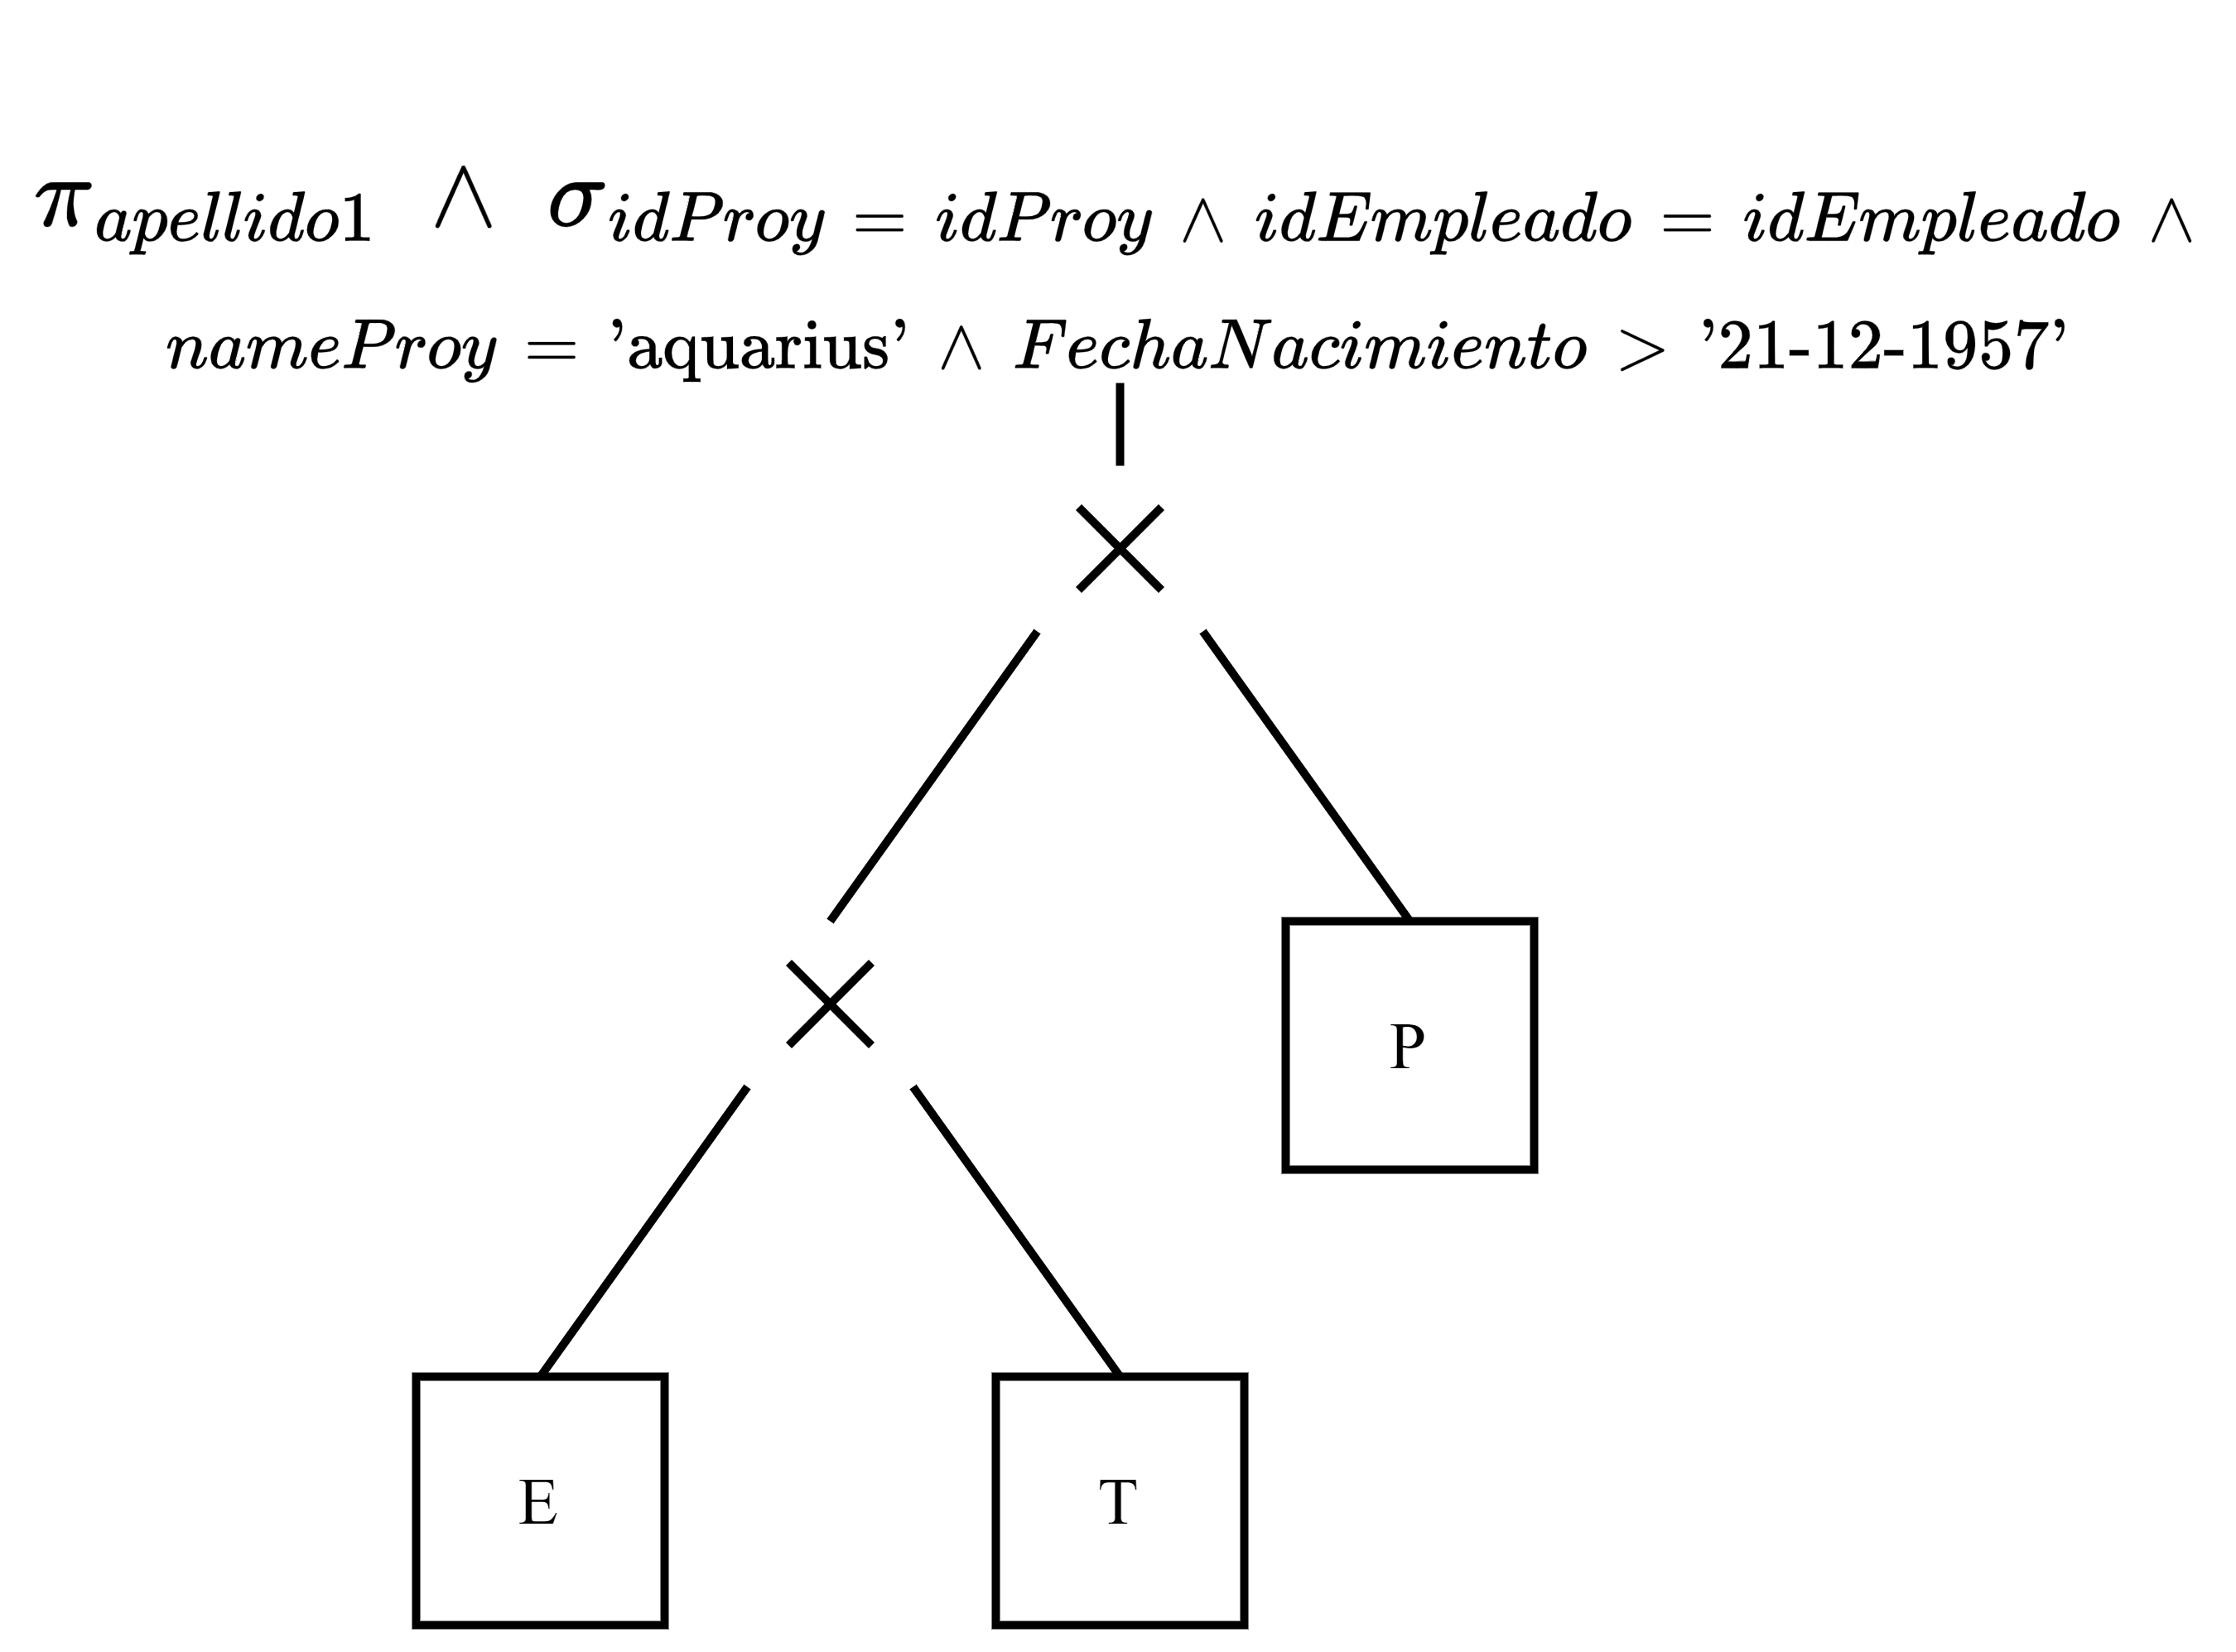
\includegraphics[width=0.8\textwidth]{img/E1-ArbolCanonico.png}
        \end{figure}

        \newpage
        \item Explique como se optimiza el árbol de consulta mediante la optimización vista en clases.
        \begin{enumerate}
            \item Se separa la proyección y las selecciones por tablas.
            \begin{figure}[H]
                \centering
                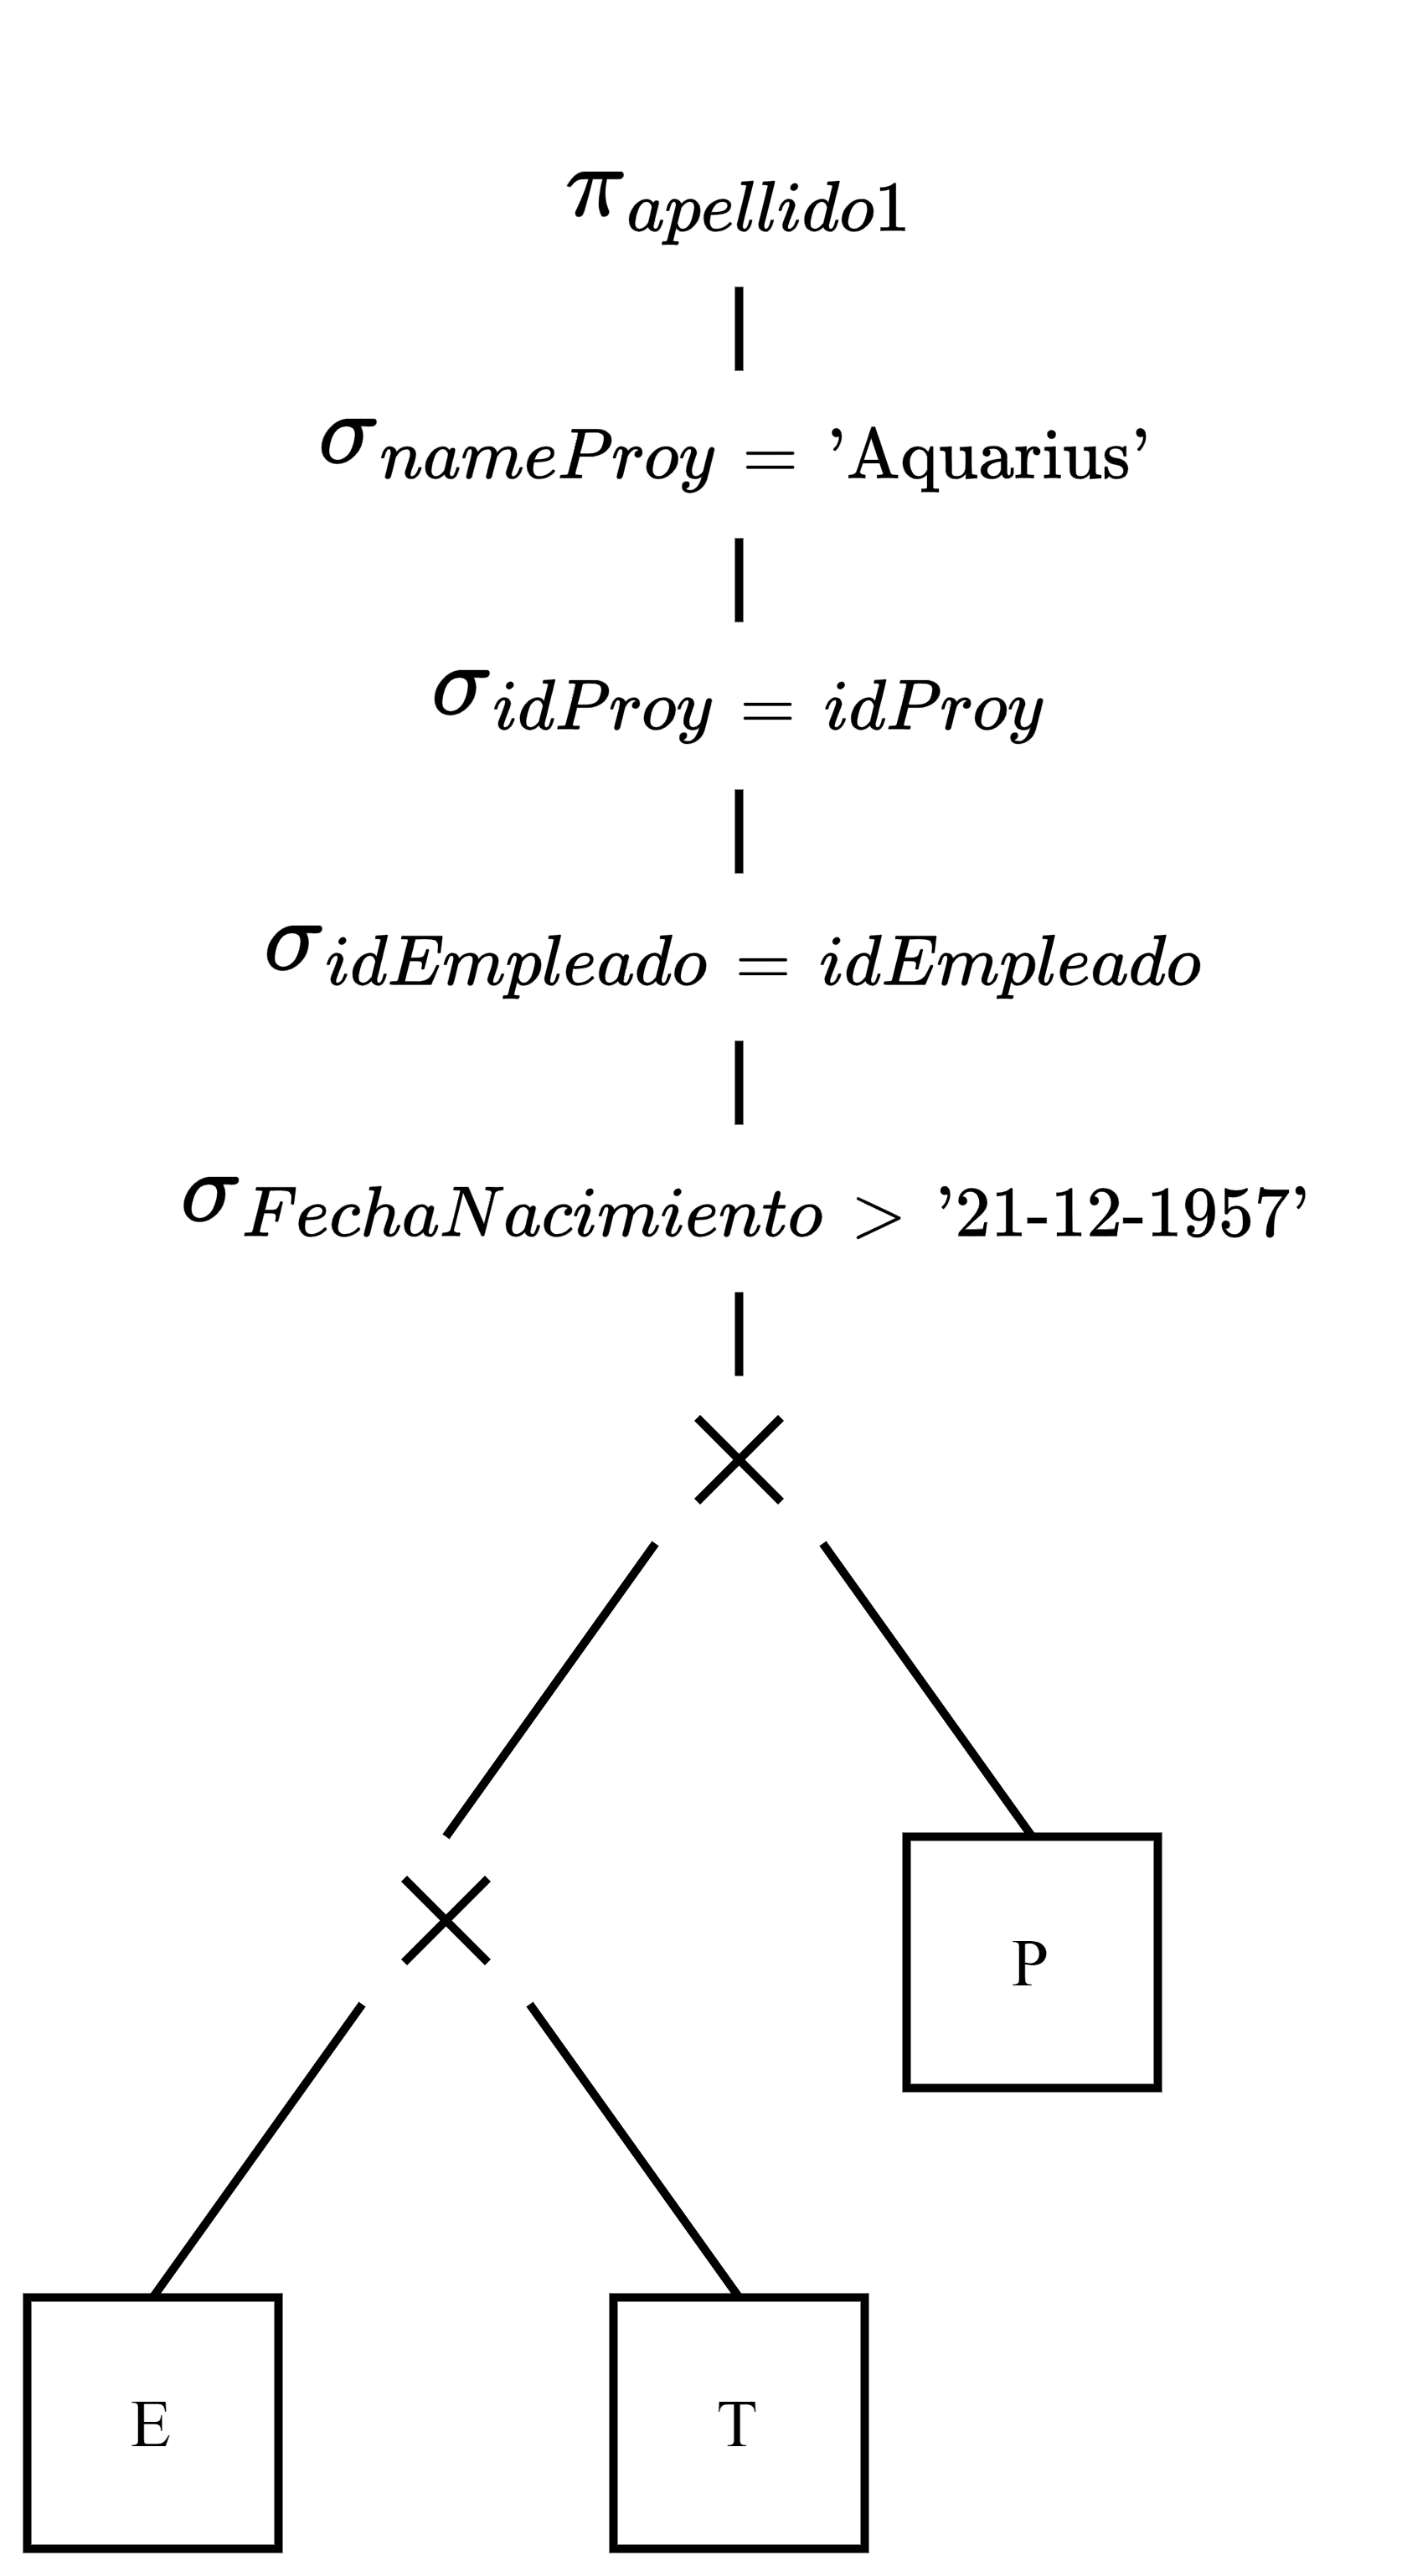
\includegraphics[width=0.45\textwidth]{img/E1-Paso1.png}
            \end{figure}

            \newpage
            \item Se reorganizan las tablas buscando la forma más optimas de unir las tablas (Solo si es posible).
            \begin{figure}[H]
                \centering
                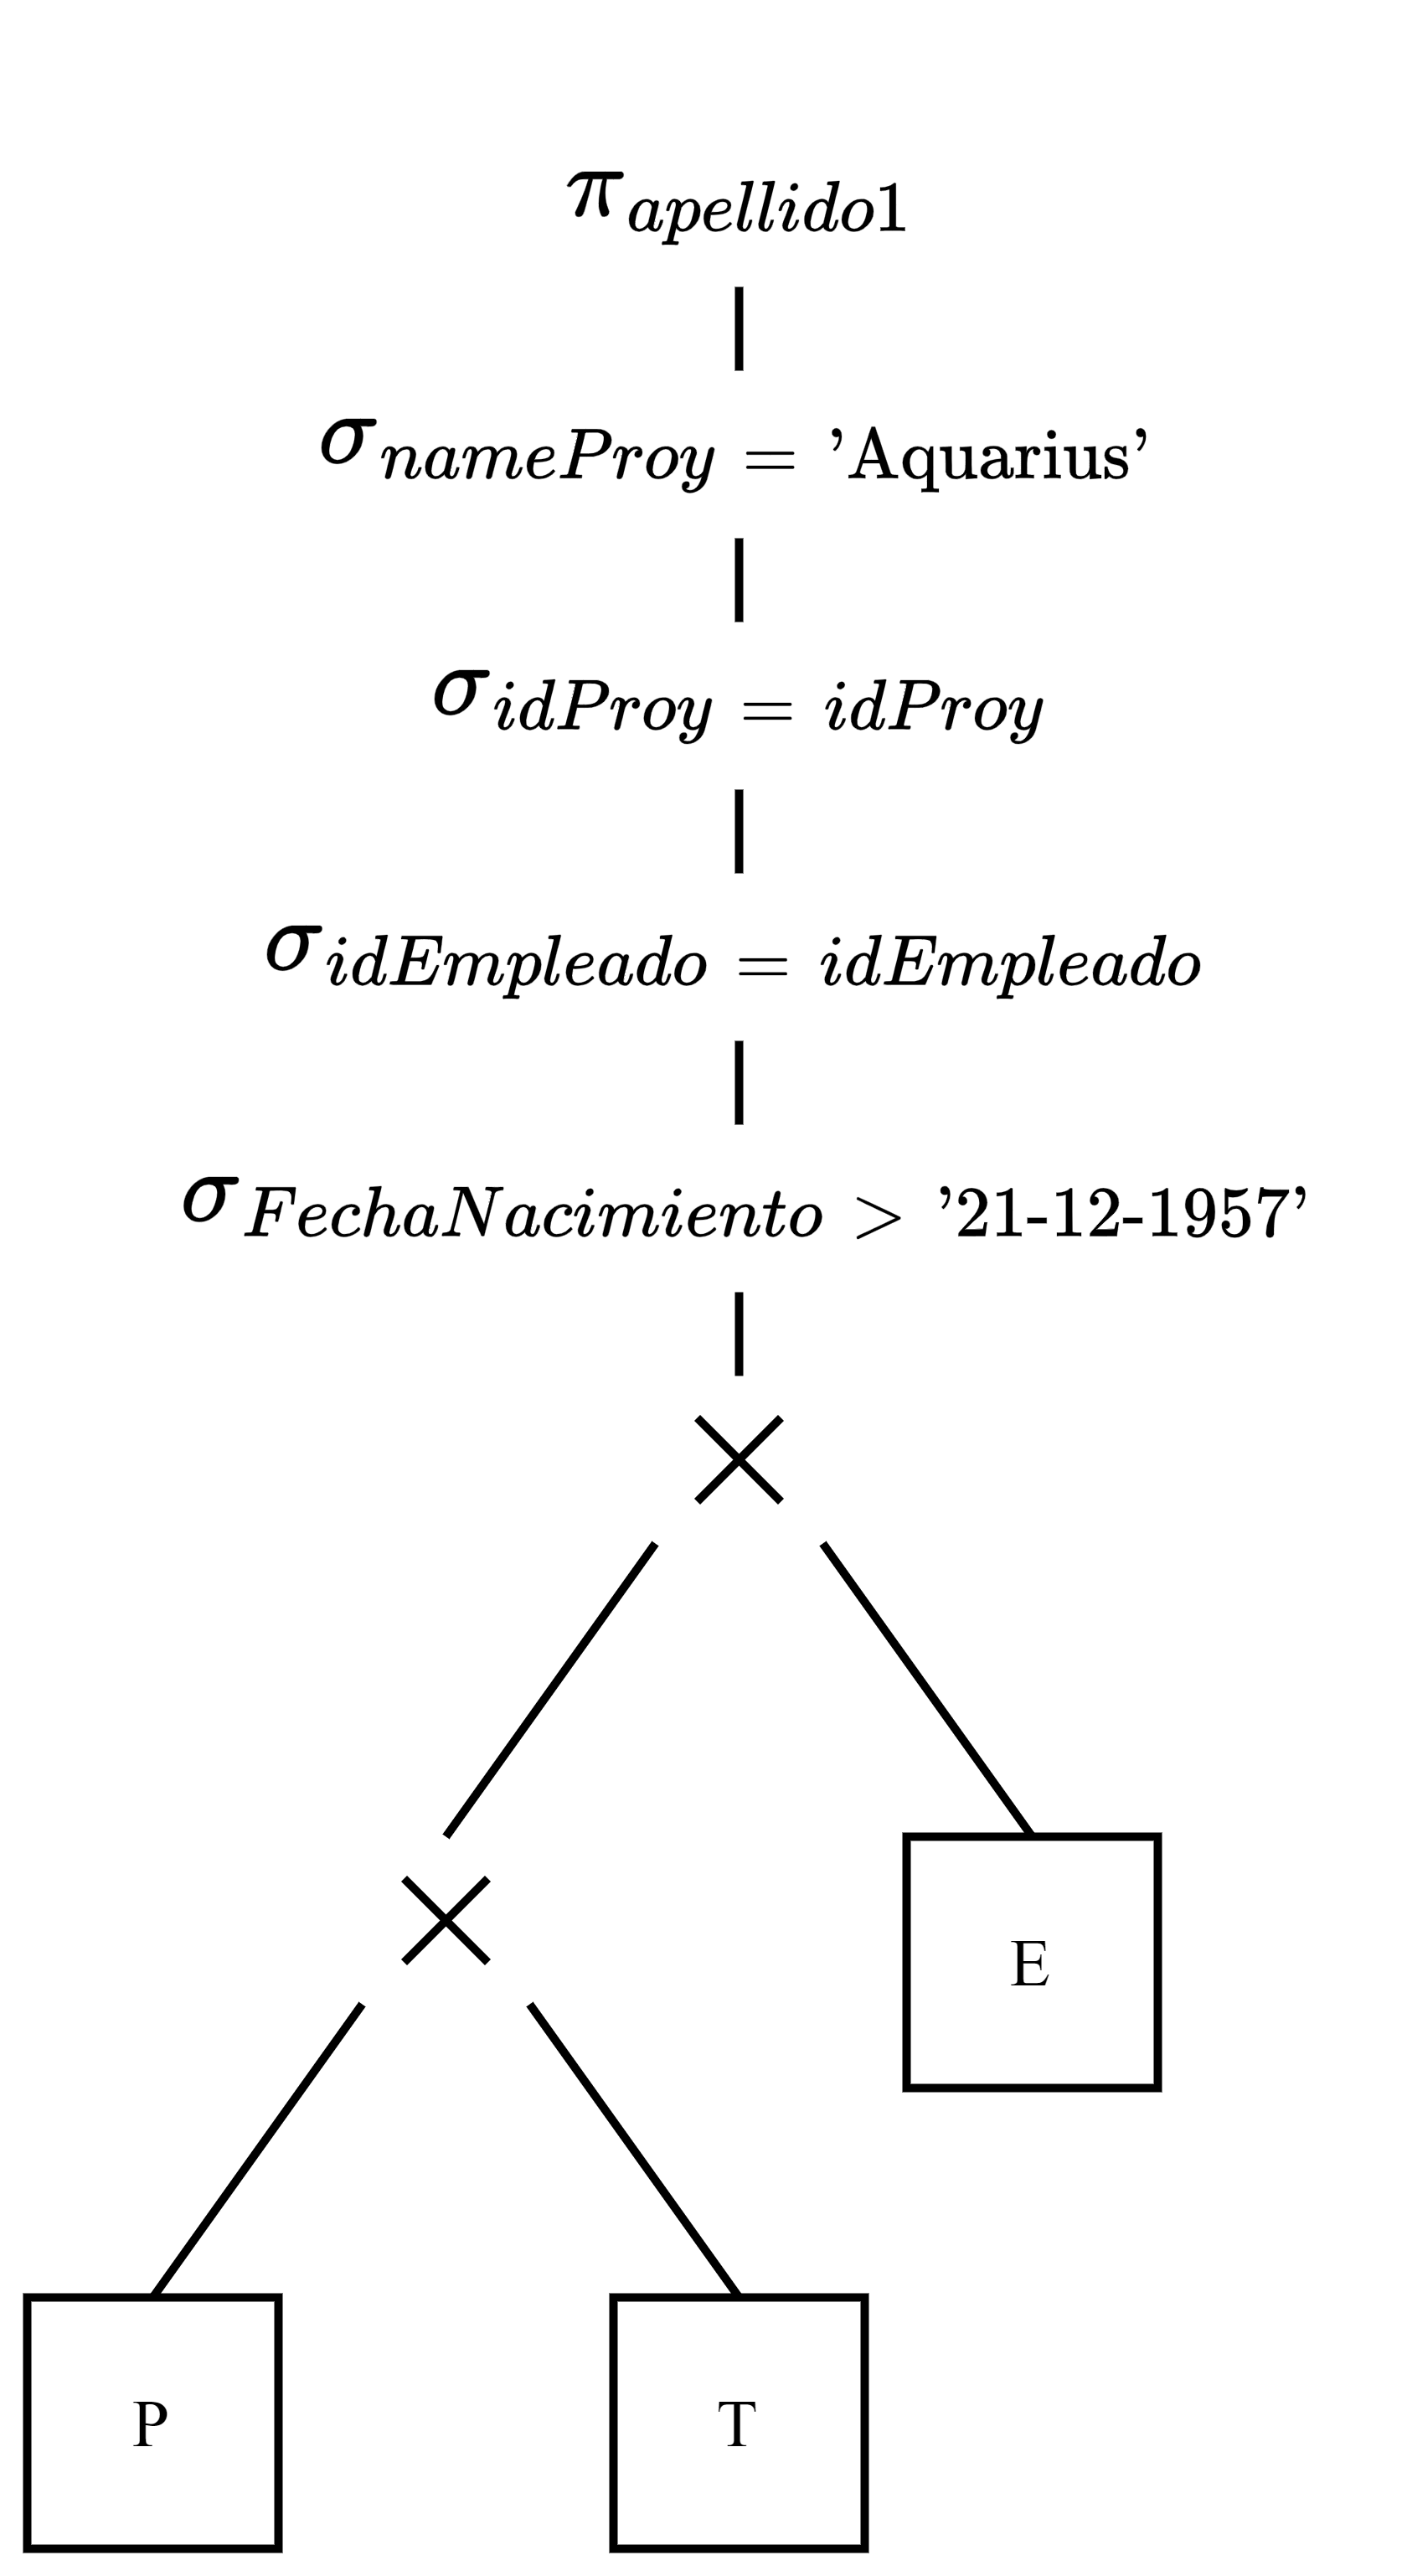
\includegraphics[width=0.35\textwidth]{img/E1-Paso2.png}
            \end{figure}

            \item Se bajan las selecciones hasta su respectivo producto cartesiano.
            \begin{figure}[H]
                \centering
                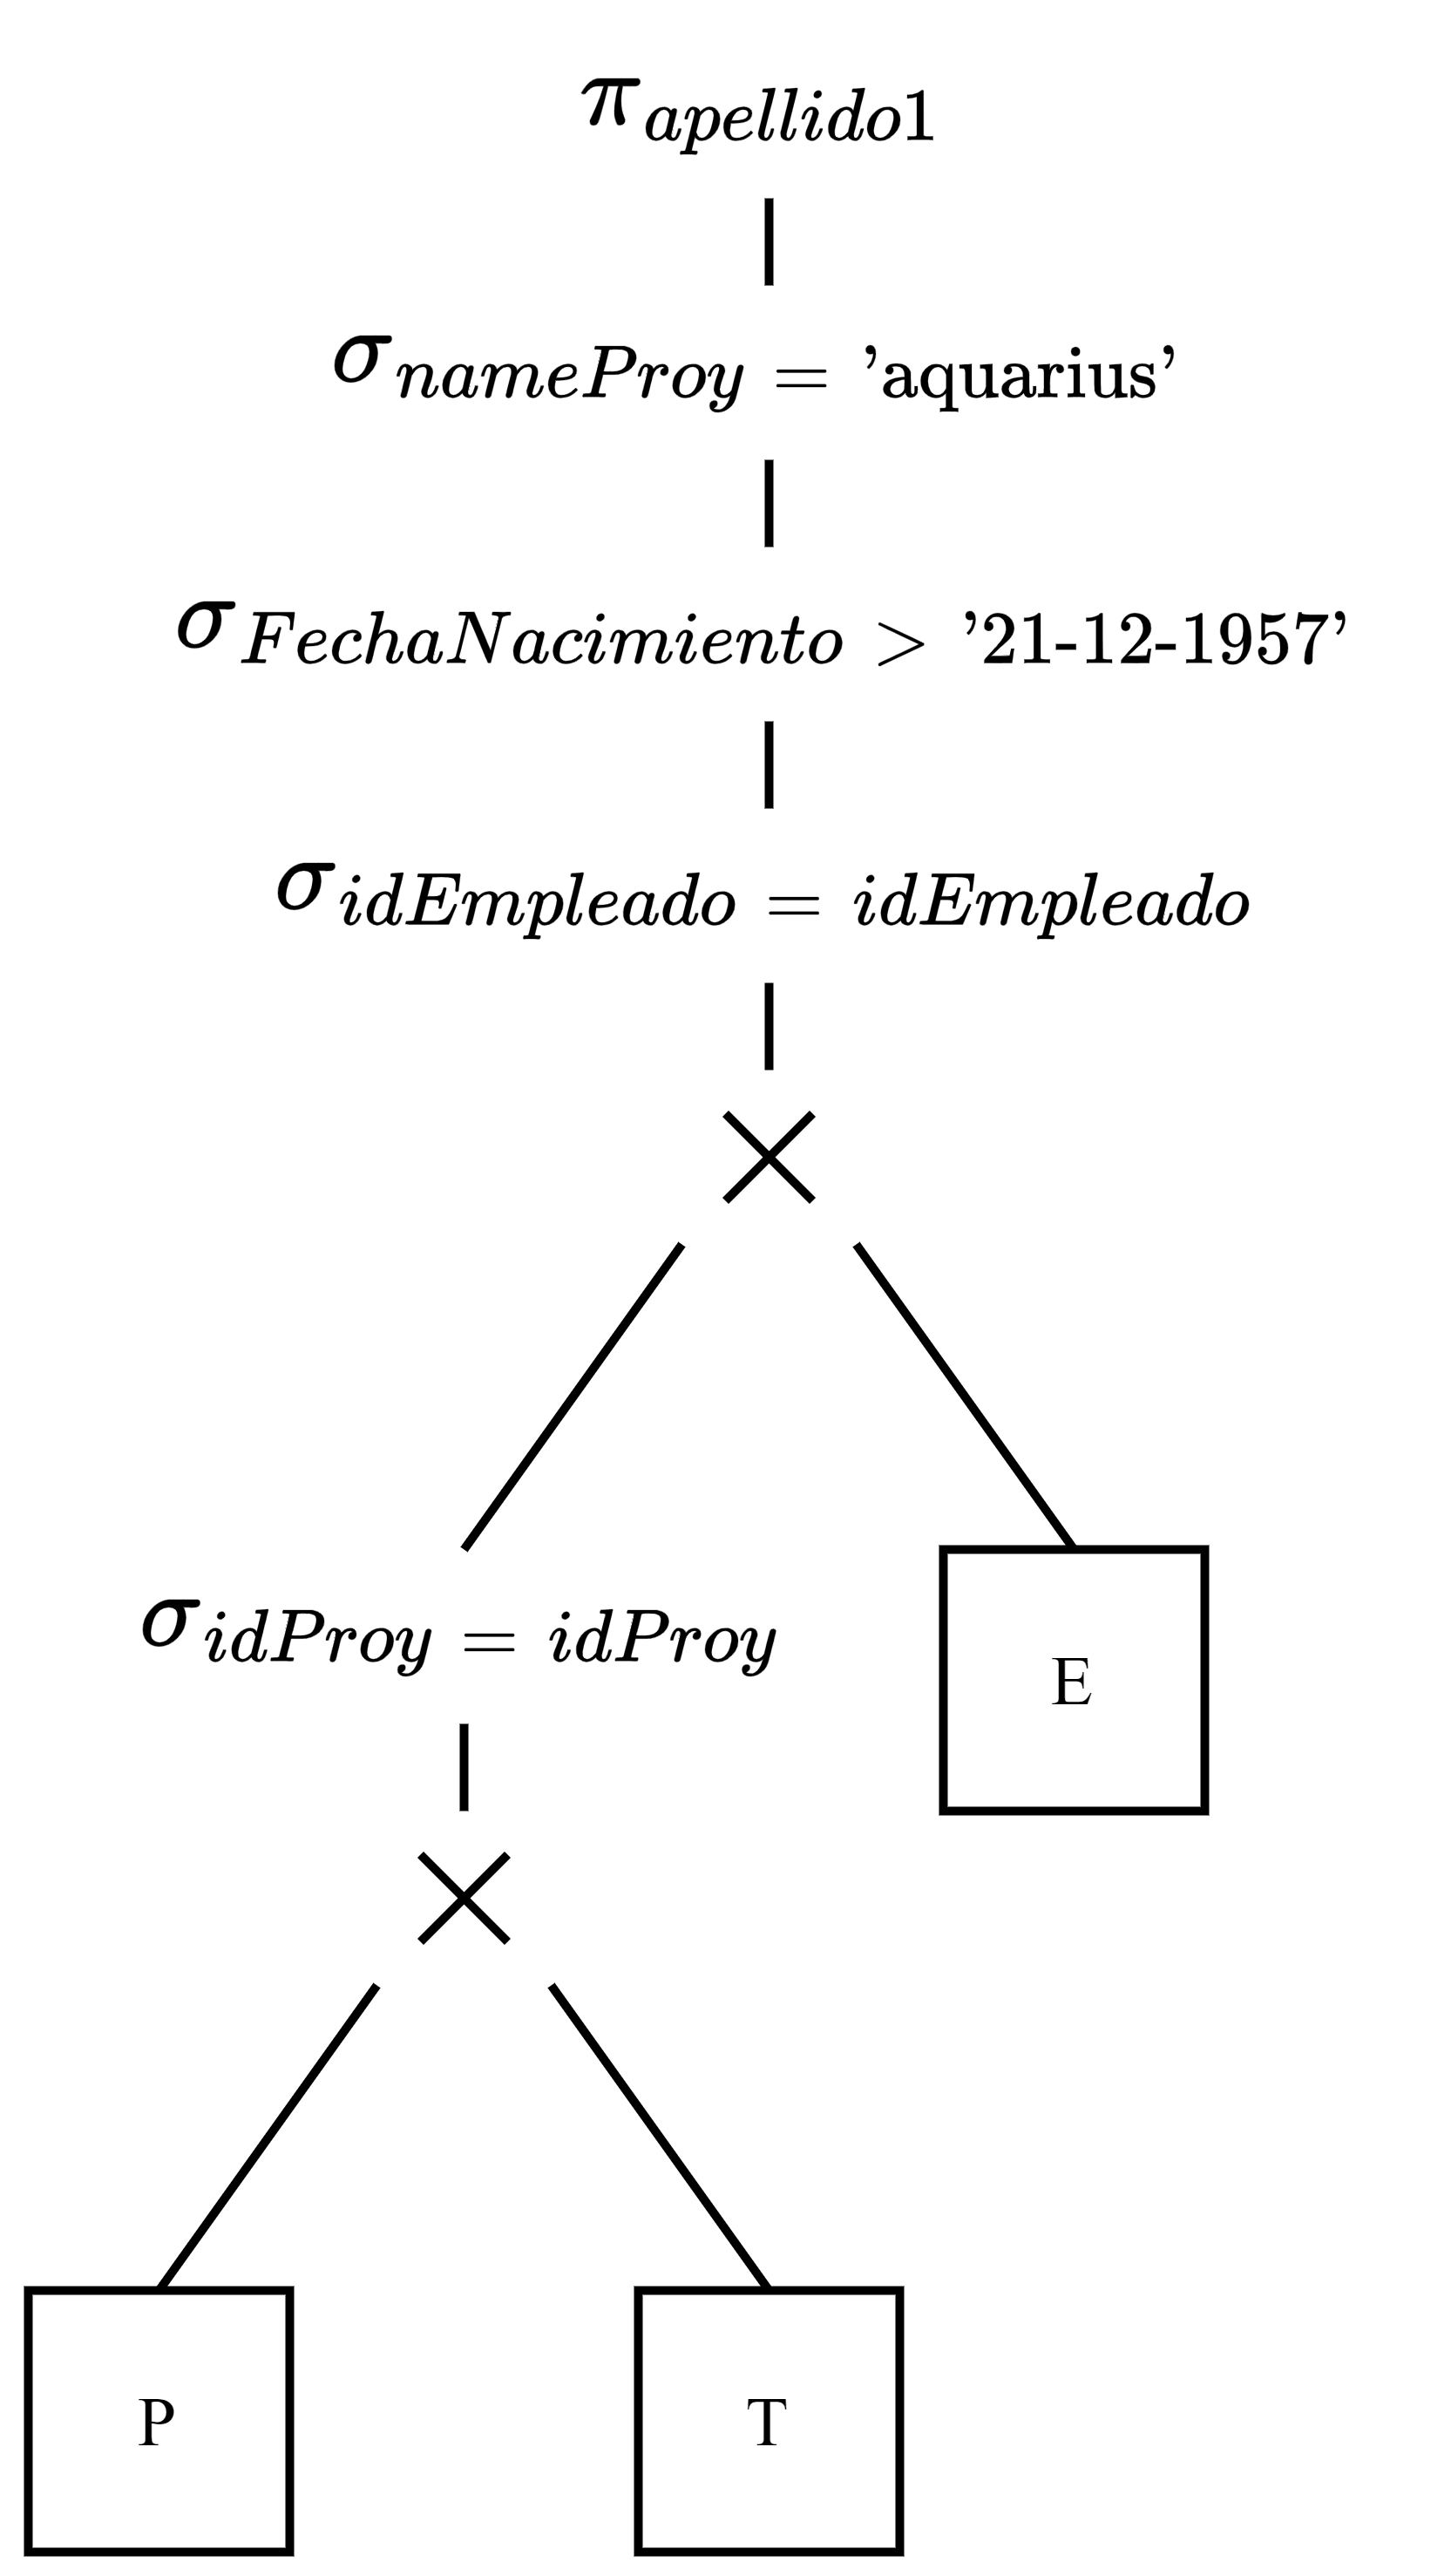
\includegraphics[width=0.35\textwidth]{img/E1-Paso3.png}
            \end{figure}

            \newpage
            \item Se cambia la seleccion y el producto cartesiano, por un join.
            \begin{figure}[H]
                \centering
                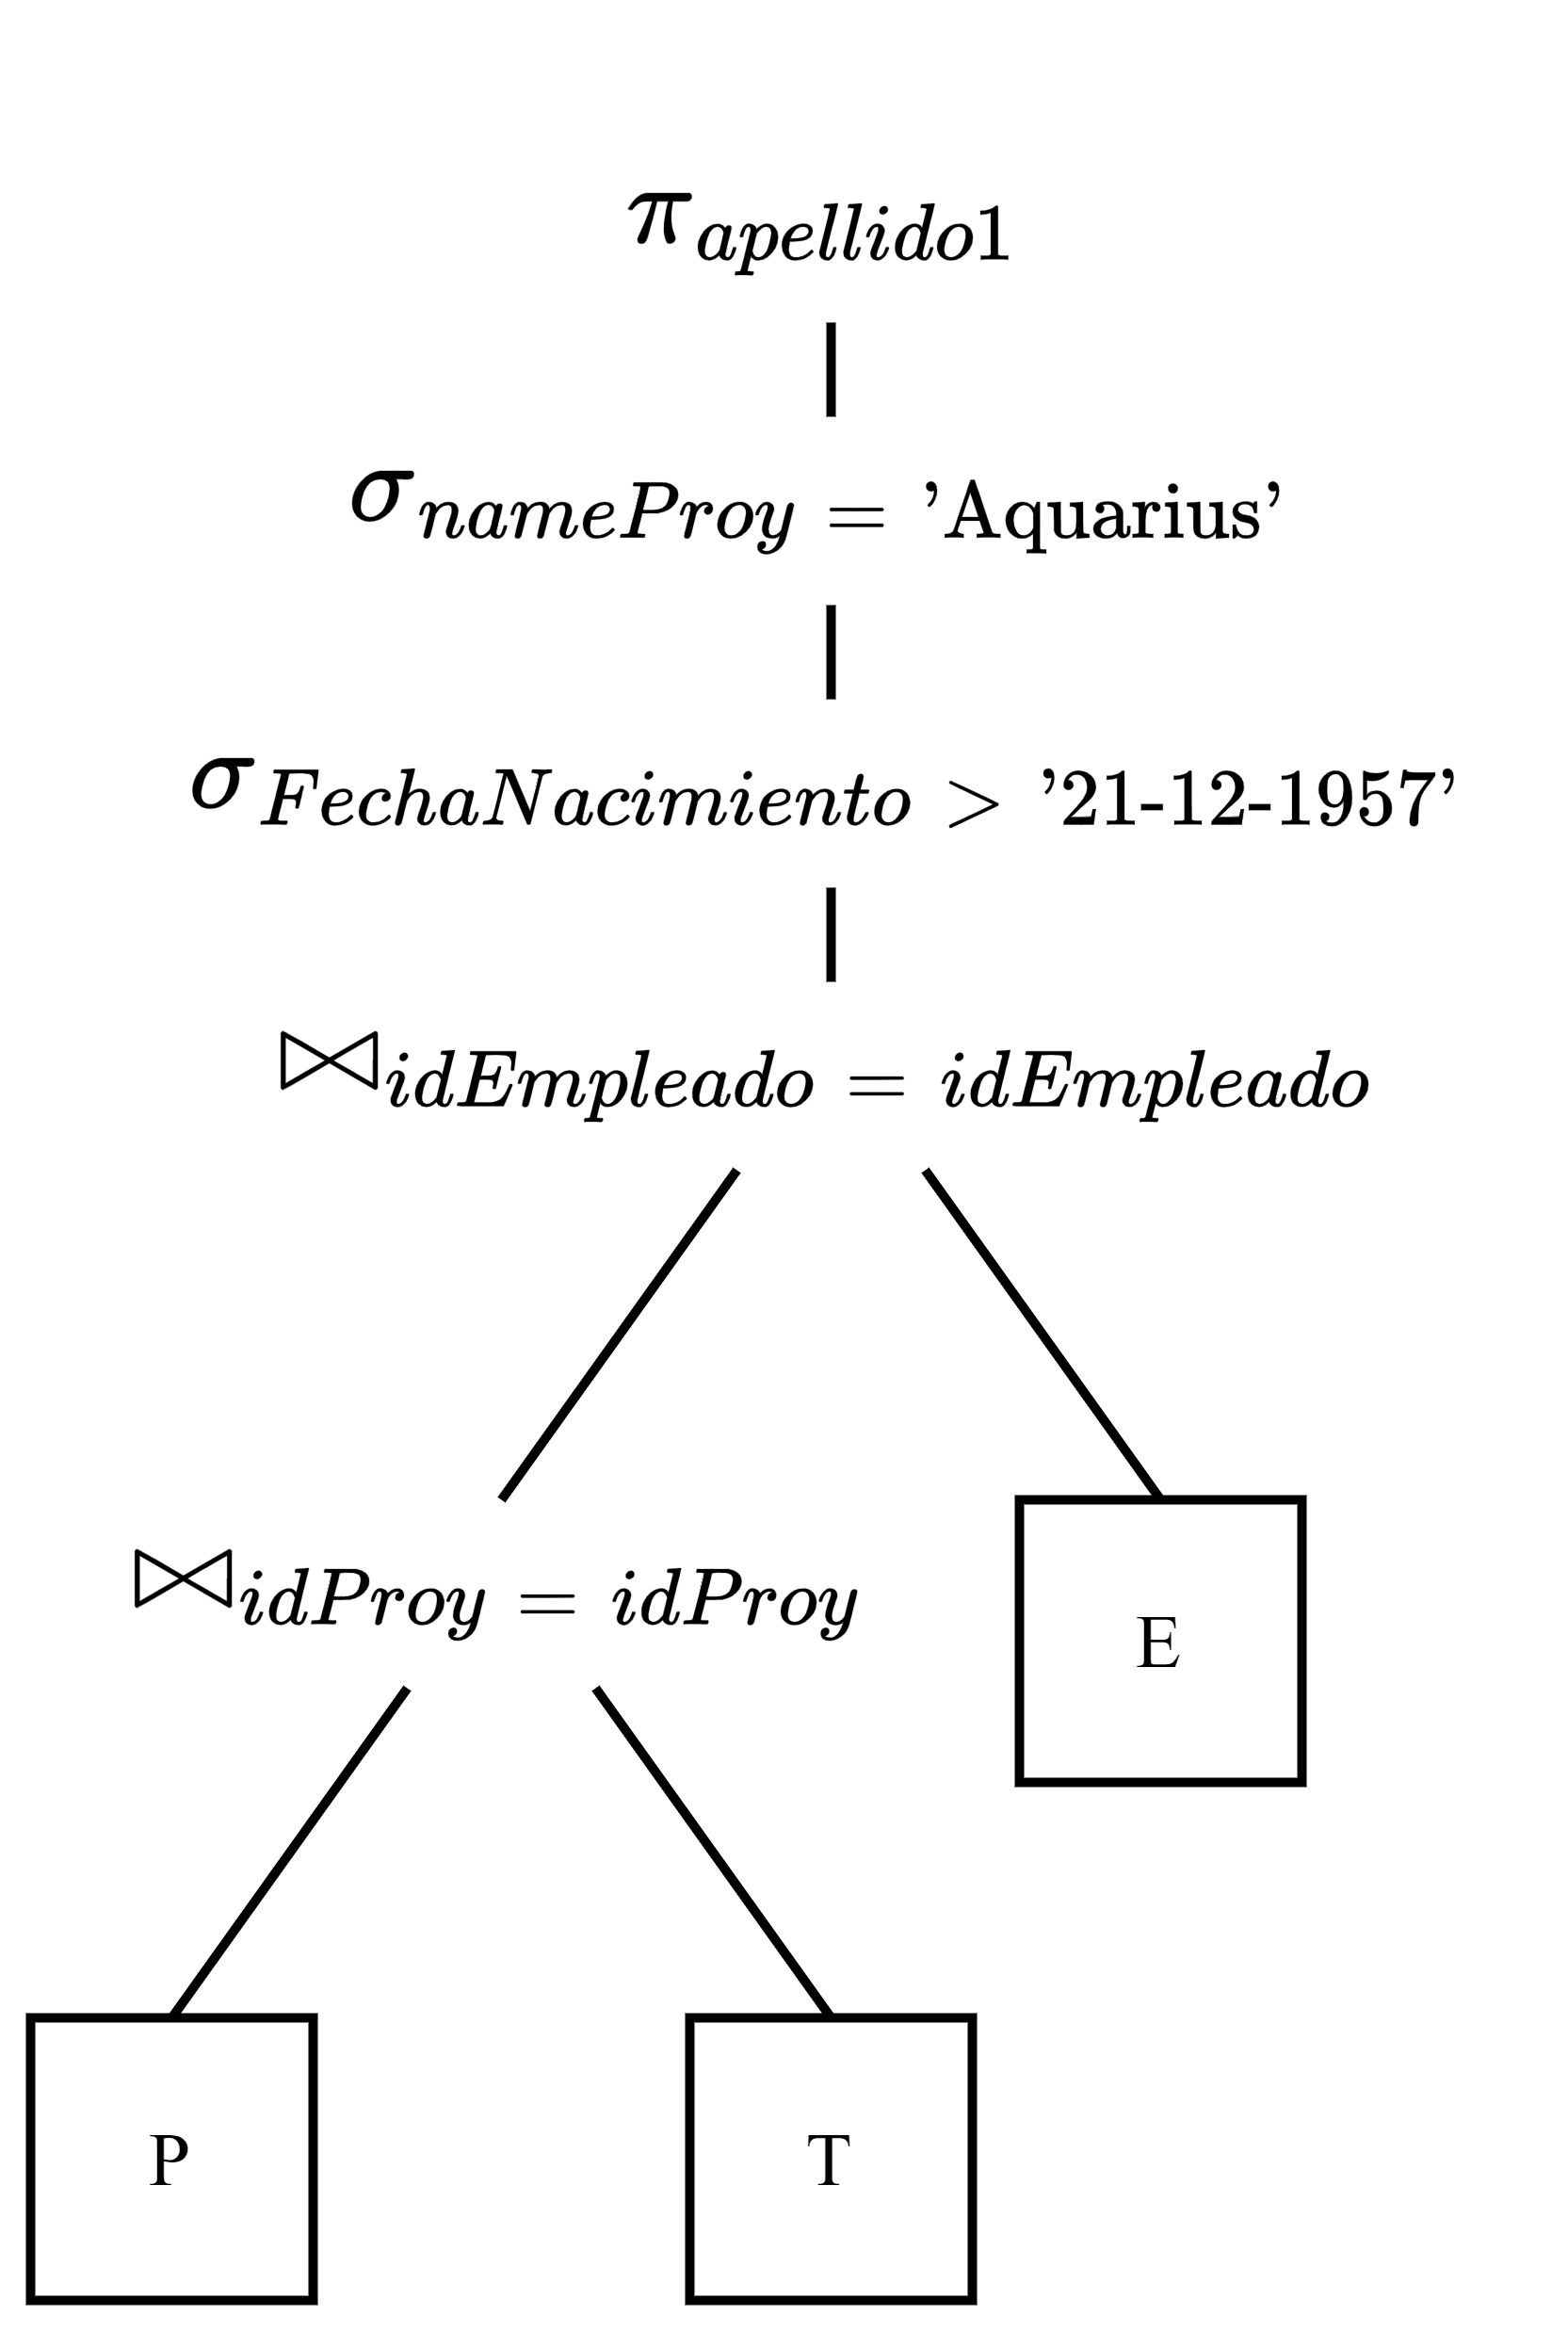
\includegraphics[width=0.4\textwidth]{img/E1-Paso4.png}
            \end{figure}

            \item Se bajan las demas selecciones a sus respectivas tablas.
            \begin{figure}[H]
                \centering
                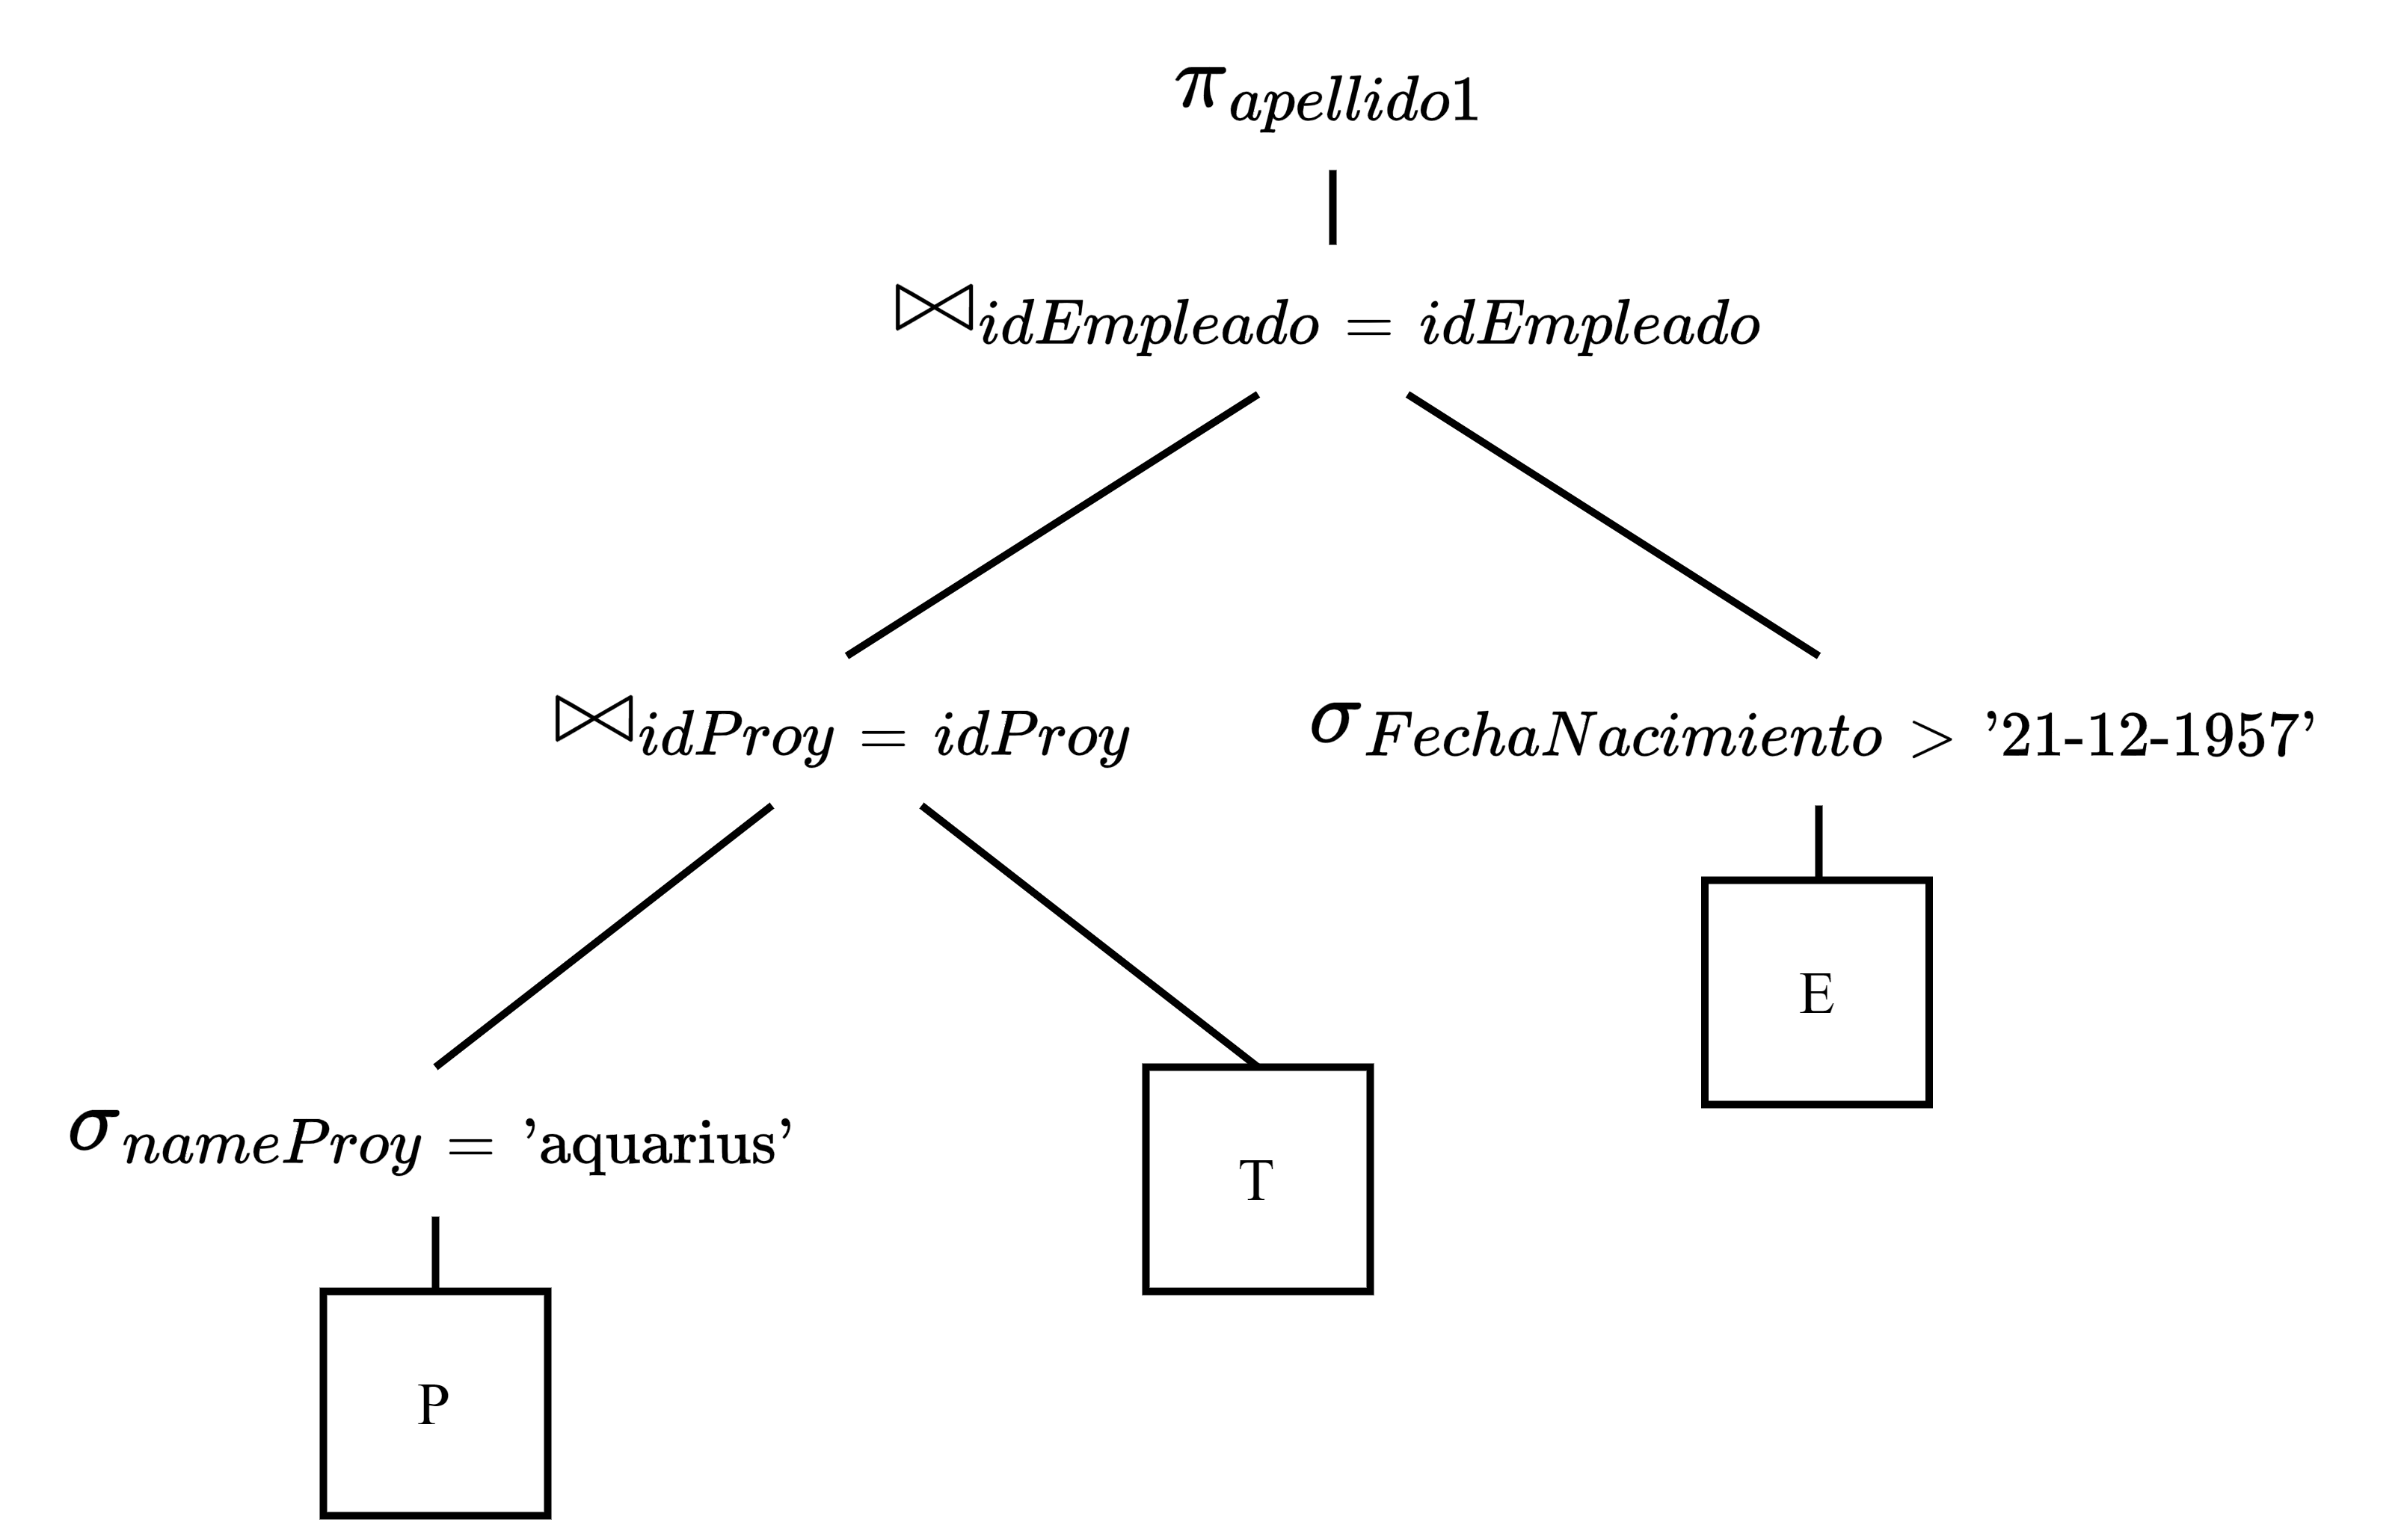
\includegraphics[width=0.8\textwidth]{img/E1-Paso5.png}
            \end{figure}

            \newpage
            \item Se proyecta solo lo necesario en las sub-tablas.
            \begin{figure}[H]
                \centering
                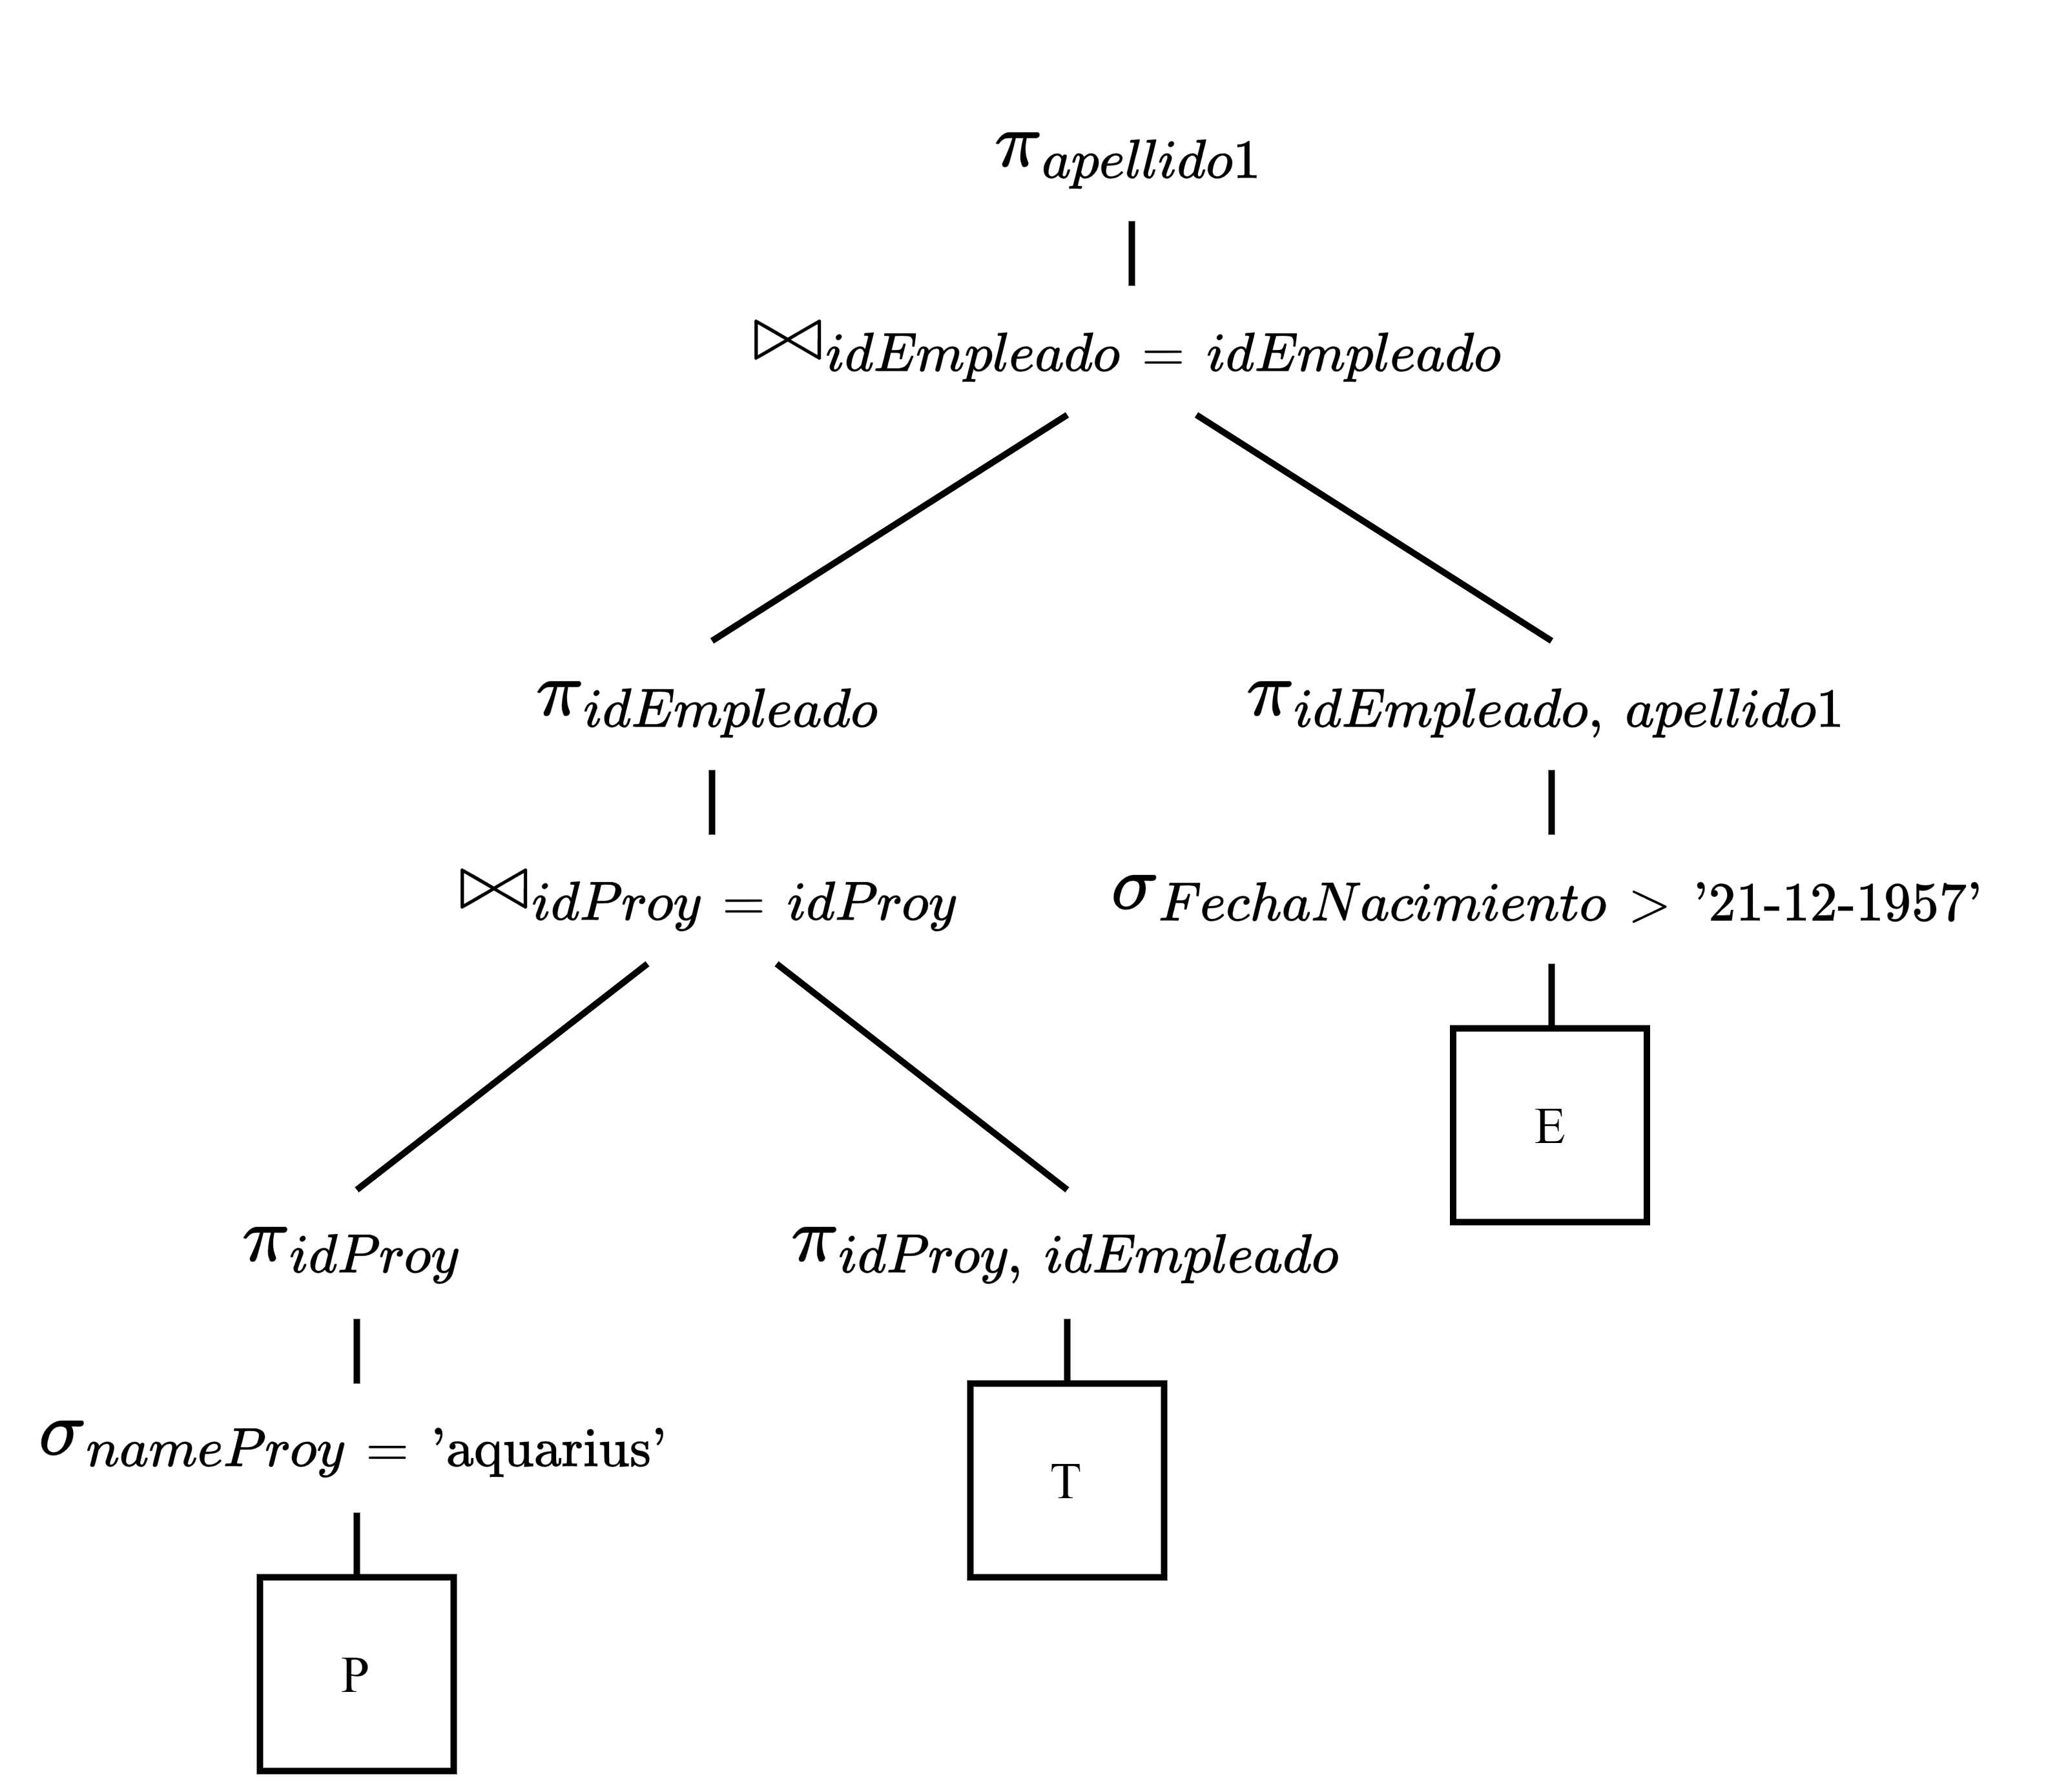
\includegraphics[width=\textwidth]{img/E1-Paso6.png}
            \end{figure}
        \end{enumerate}
    \end{enumerate}

    \newpage
    \item Considere las siguientes relaciones:
    \begin{itemize}
        \item \textbf{Variedades}(IdVar, Nombre, Prog2, Prog1)

        \item \textbf{Predios}(IdPredio, NombrePredio, Comuna, Superficie)

        \item \textbf{Siembra}(IdPredio, IdVar, HaSem, Rdto, añoA)
    \end{itemize}
    Sea la siguiente consulta: \newline
    \textit{"Listar los nombres de las variedades sembradas en el predio IdPredio = 10 y que el año 2015 tuvieron un rendimiento mayor a 60 qq/ha."}
    \begin{enumerate}
        \item Escriba la consulta SQL para la consulta anterior.
        \begin{tcolorbox}[
            colback=Verde!30,
            colframe=Verde!90!black]
            \begin{verbatim}
SELECT Nombre
FROM Variedades V, Siembra S
WHERE S.IdPredio = 10
AND V.IdVar = S.IdVar
AND S.añoA = 2015
AND S.Rdto > 60;
            \end{verbatim}
        \end{tcolorbox}
        \item Escriba la consulta en Algebra Relacional para la consulta anterior.
        \begin{align*}
            \scalebox{1.5}{$\pi$}_{\text{Nombre}} (
                \scalebox{1.5}{$\sigma$}_{
                    \scalebox{0.8}{
                        $\begin{array}{l}
                            \text{IdPredio} = 10 \; \wedge \\
                            \text{IdVar} = \text{IdVar} \; \wedge \\
                            \text{a\~noA} = 2015 \; \wedge \\
                            \text{Rdto} > 60
                        \end{array}$
                    }
                } (
                    \text{Variedades}_{\scalebox{1.3}{$\Join$}} \text{Siembra}
                )
            )
        \end{align*}

        \item Obtener el árbol inicial(canónico) de la consulta.
        \begin{figure}[H]
            \centering
            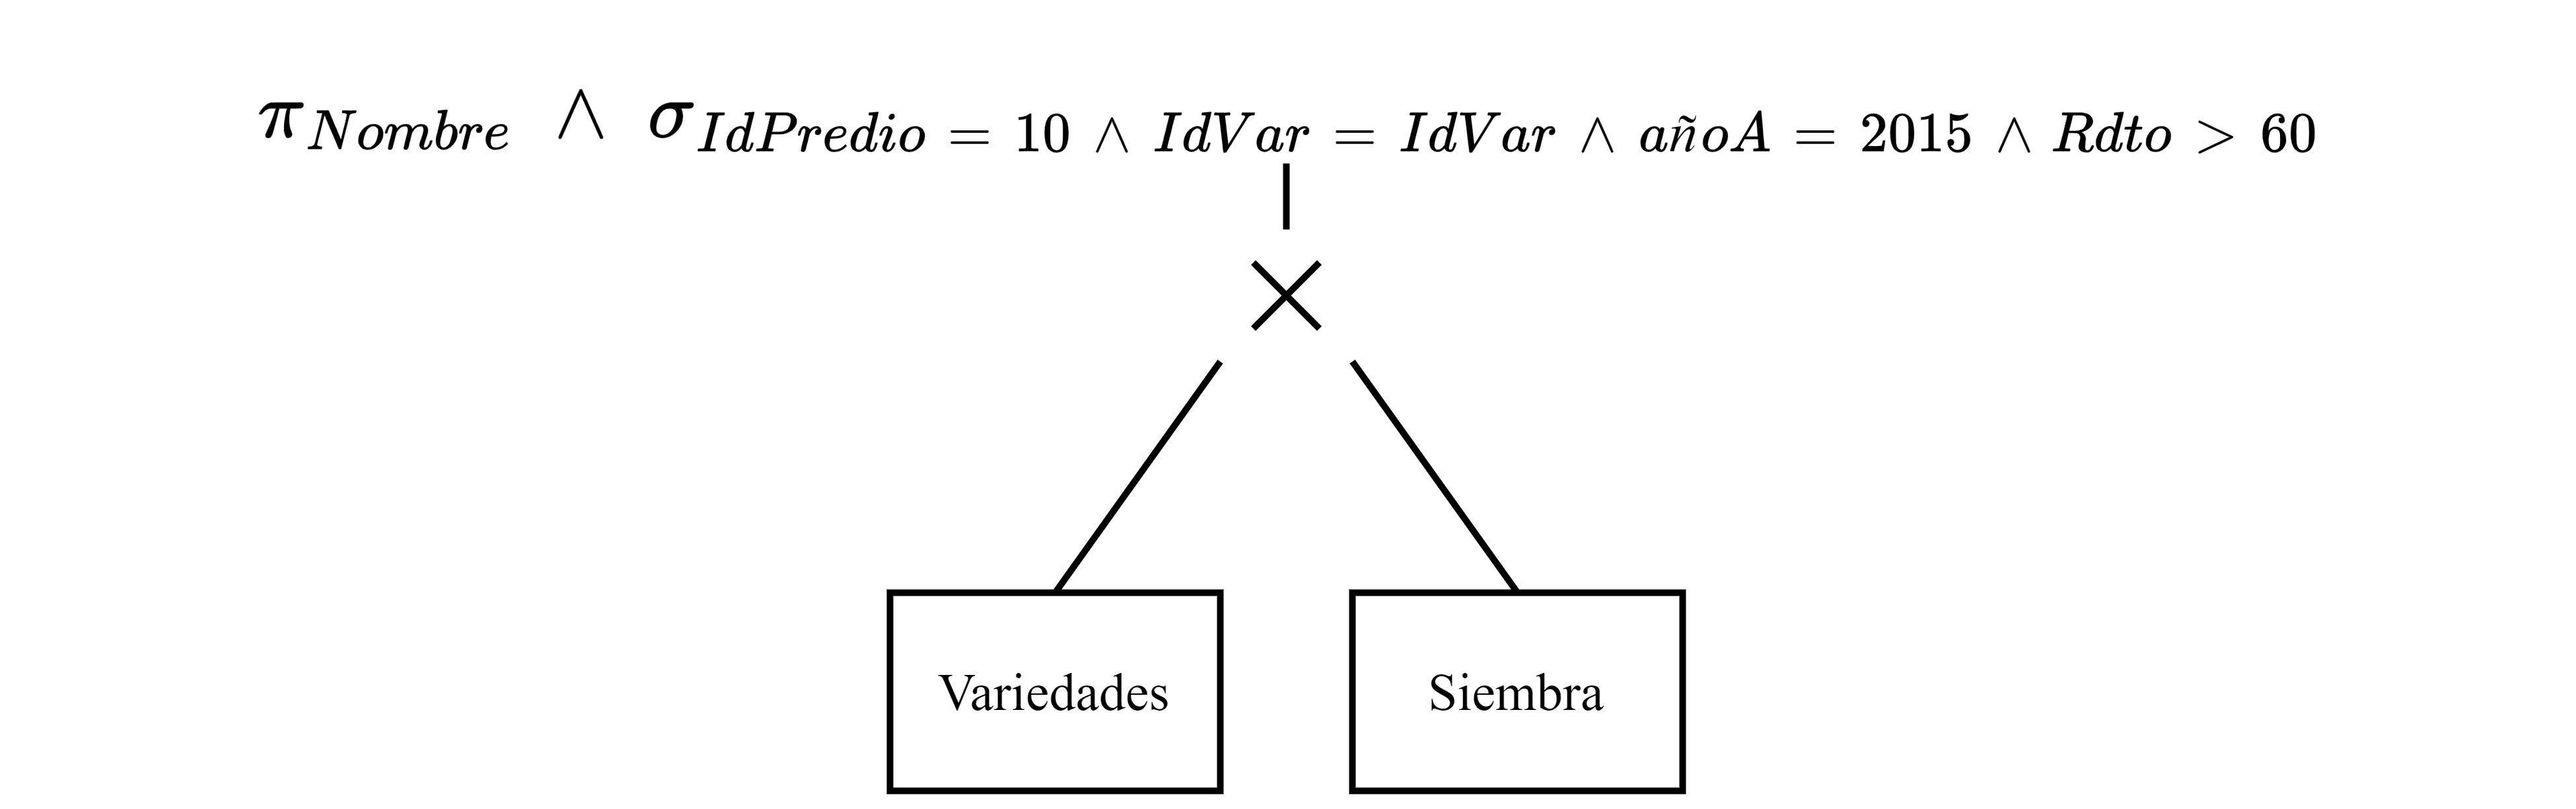
\includegraphics[width=\textwidth]{img/E2-ArbolCanonico.png}
        \end{figure}

        \newpage
        \item Explique como se optimiza el árbol de consulta mediante el algoritmo de optimización algebraica (visto en clases).
        \begin{enumerate}
            \item Se separa la proyección y las selecciones por tablas.
            \begin{figure}[H]
                \centering
                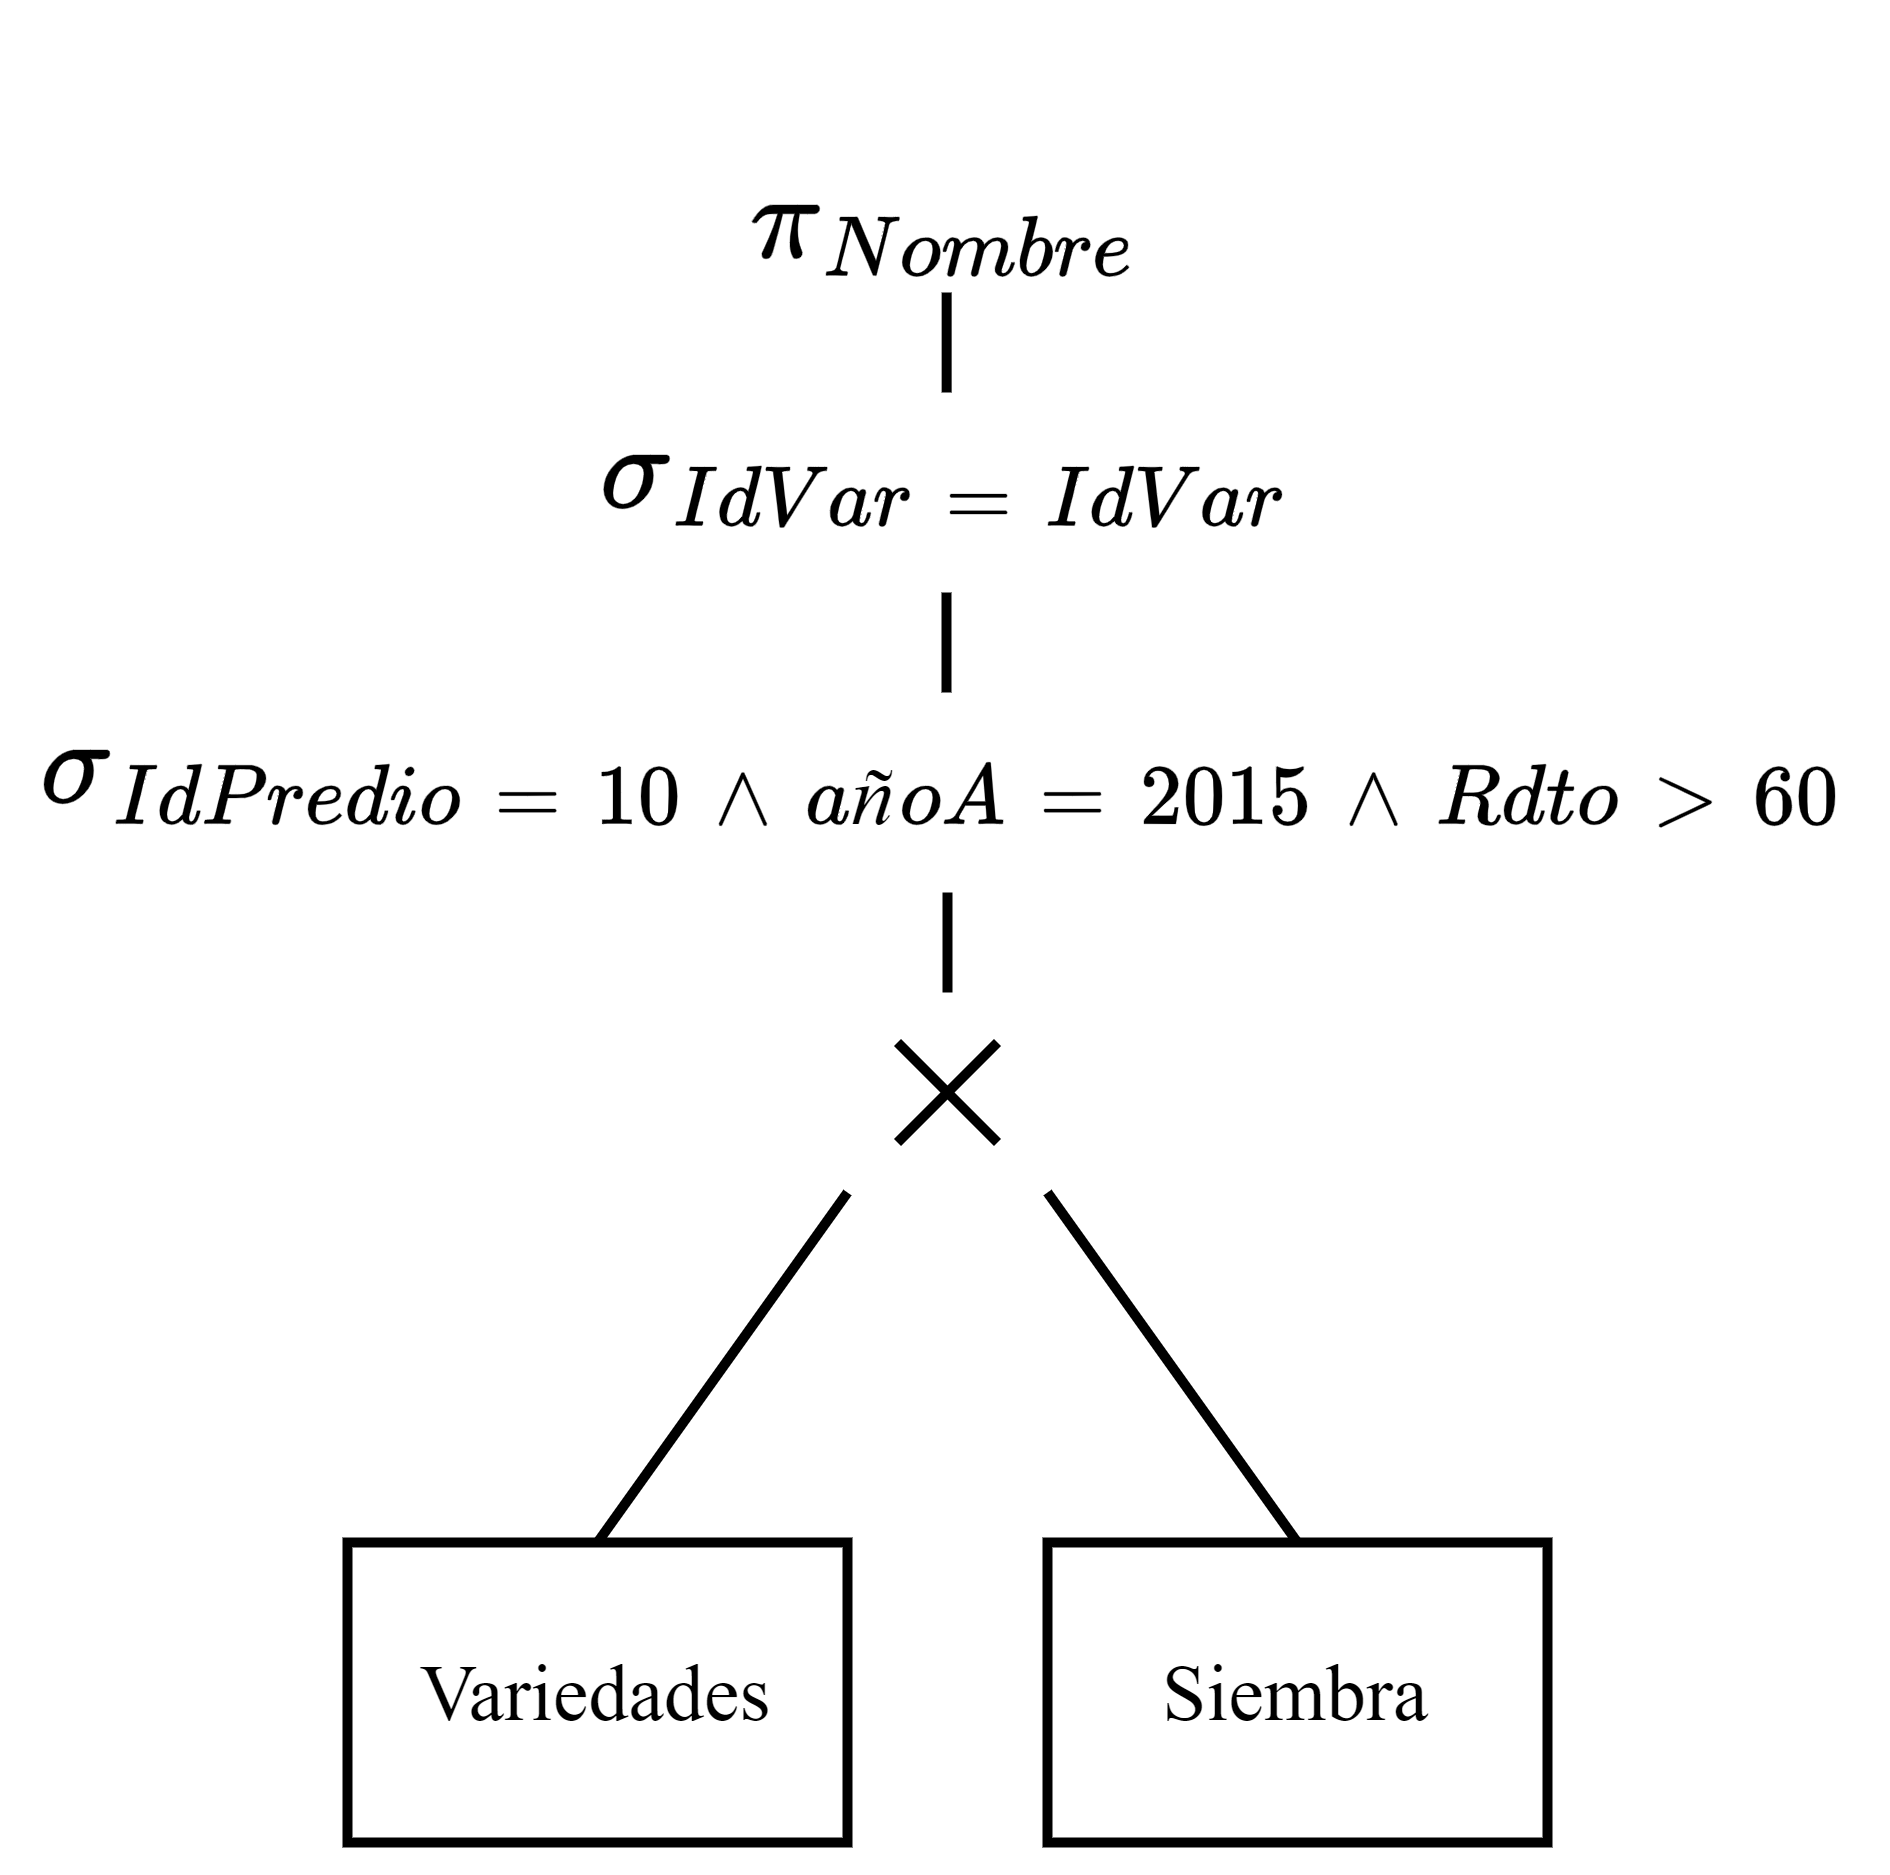
\includegraphics[width=0.6\textwidth]{img/E2-Paso1.png}
            \end{figure}

            \item Se reorganizan las tablas buscando la forma más optimas de unir las tablas (Solo si es posible).

            \item Se bajan las selecciones hasta su respectivo producto cartesiano.
            \begin{figure}[H]
                \centering
                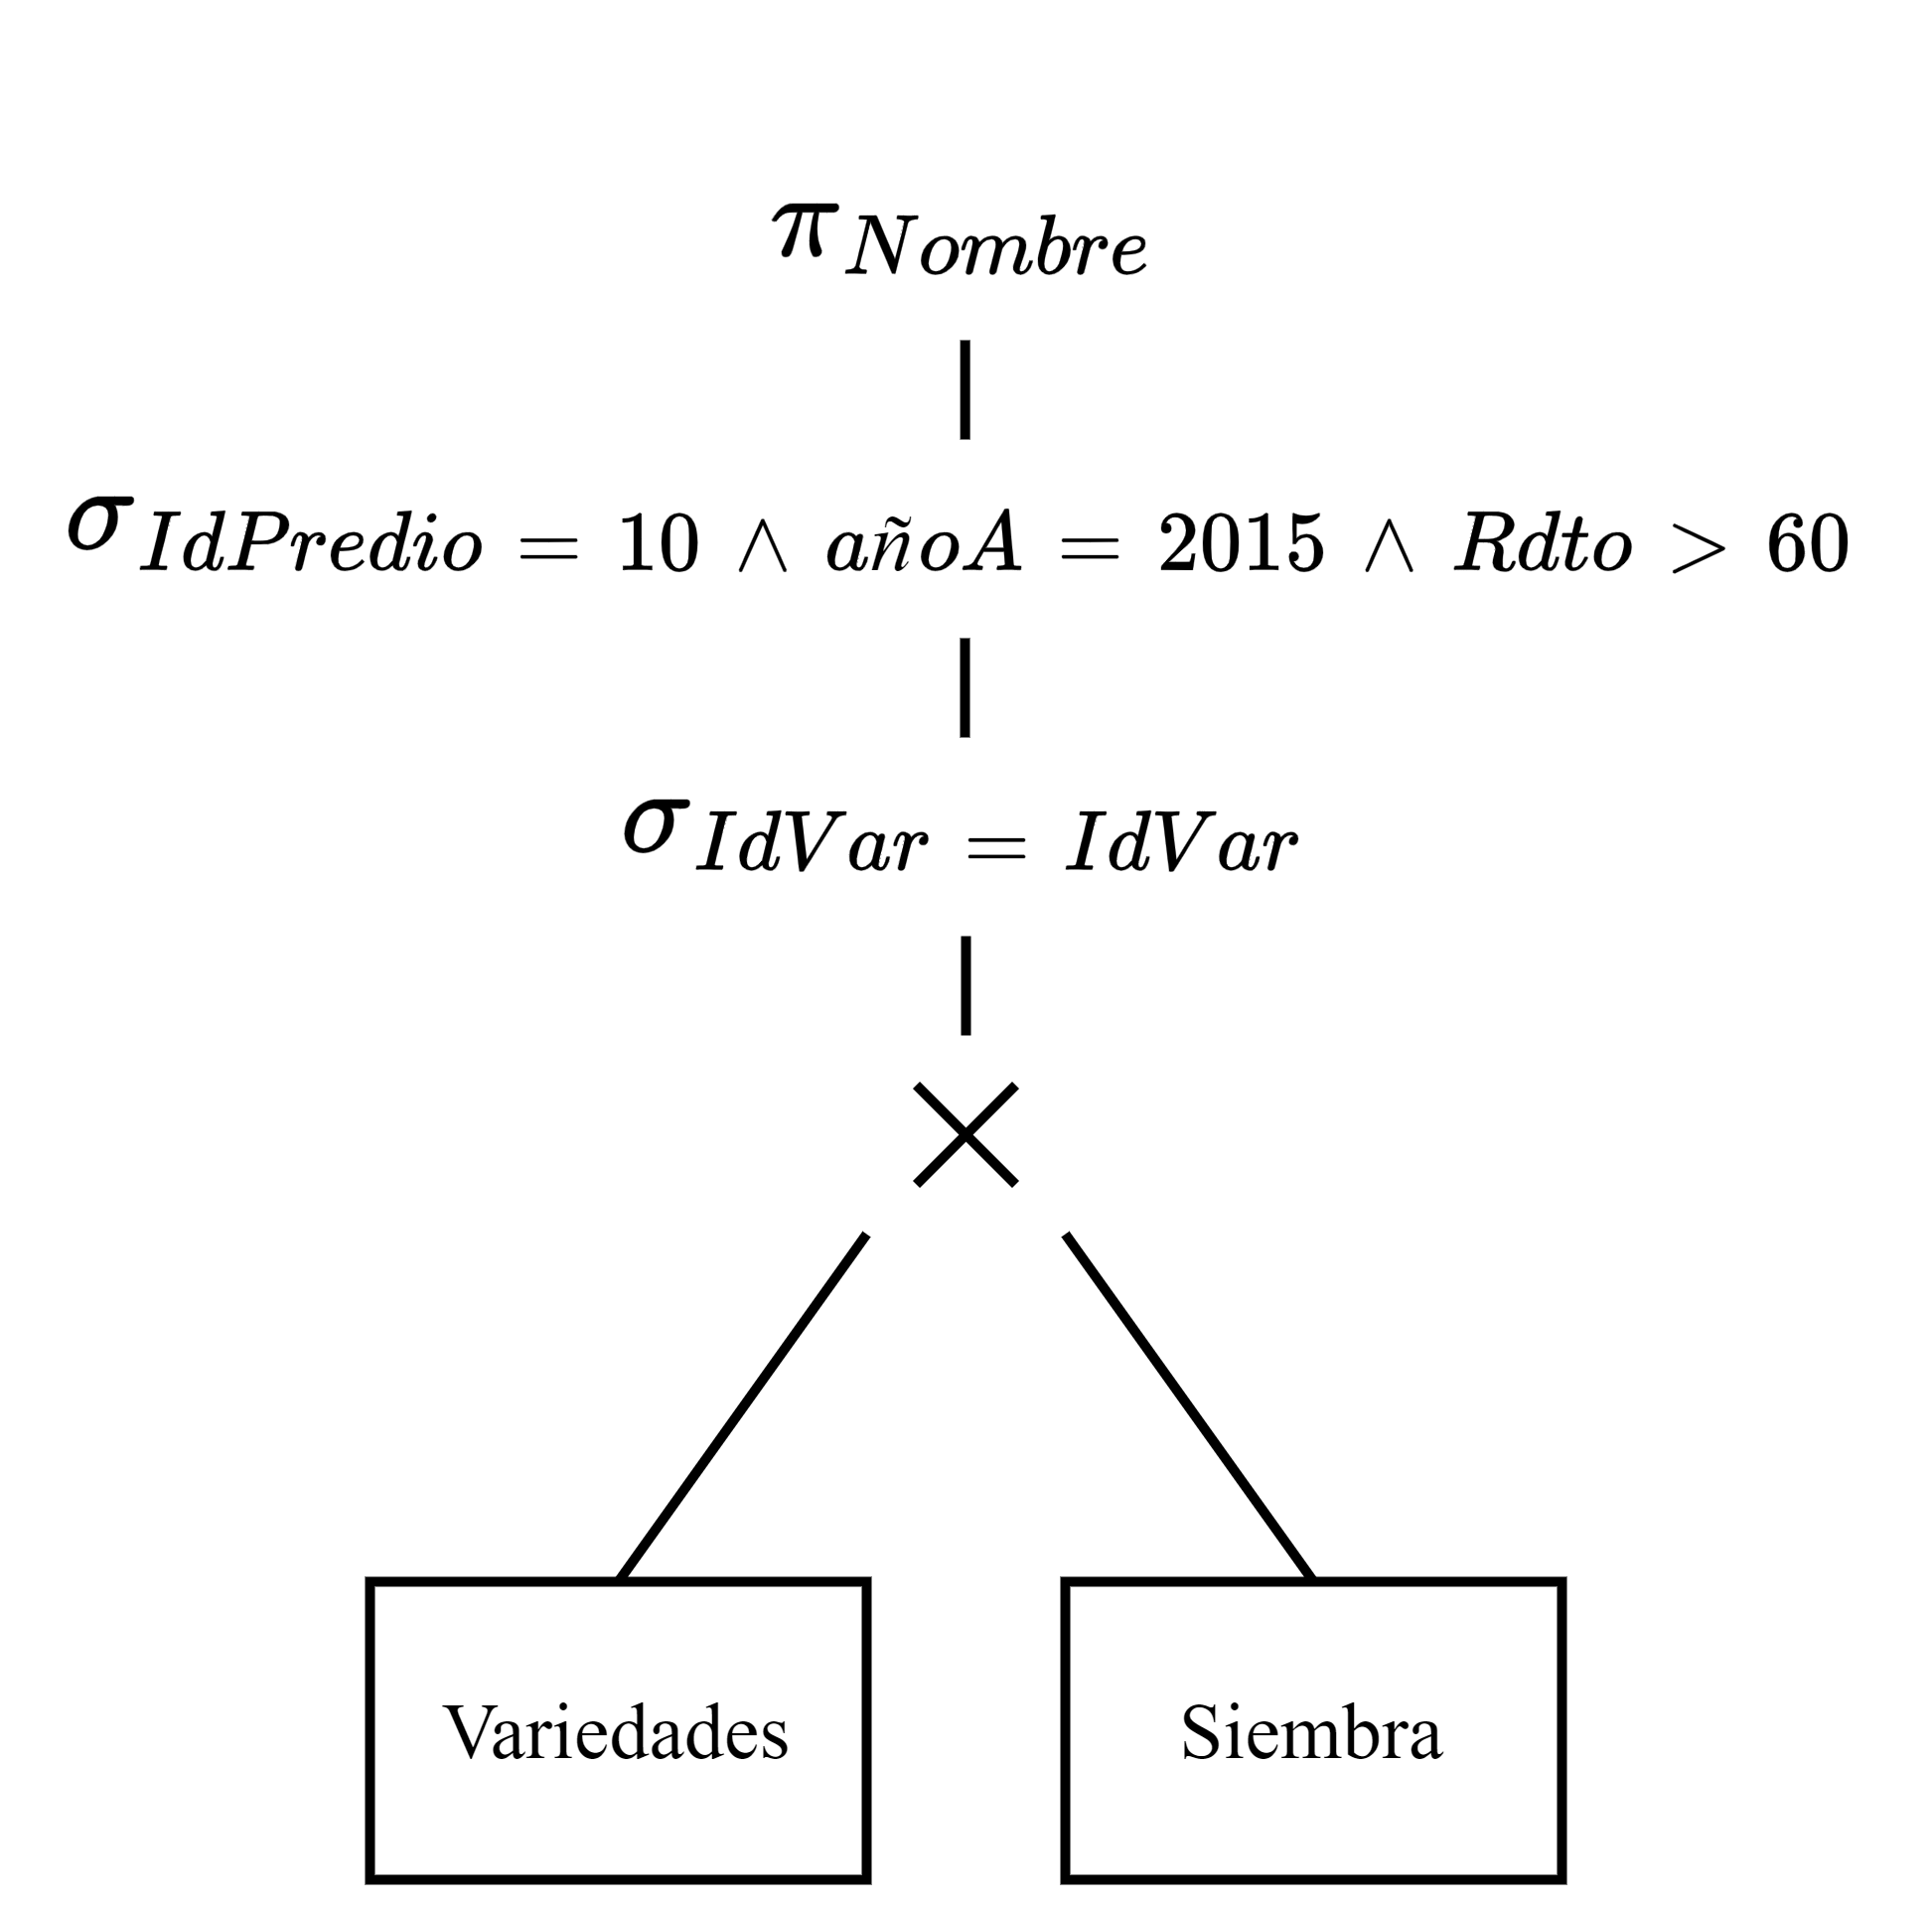
\includegraphics[width=0.6\textwidth]{img/E2-Paso3.png}
            \end{figure}

            \newpage
            \item Se cambia la seleccion y el producto cartesiano por un join.
            \begin{figure}[H]
                \centering
                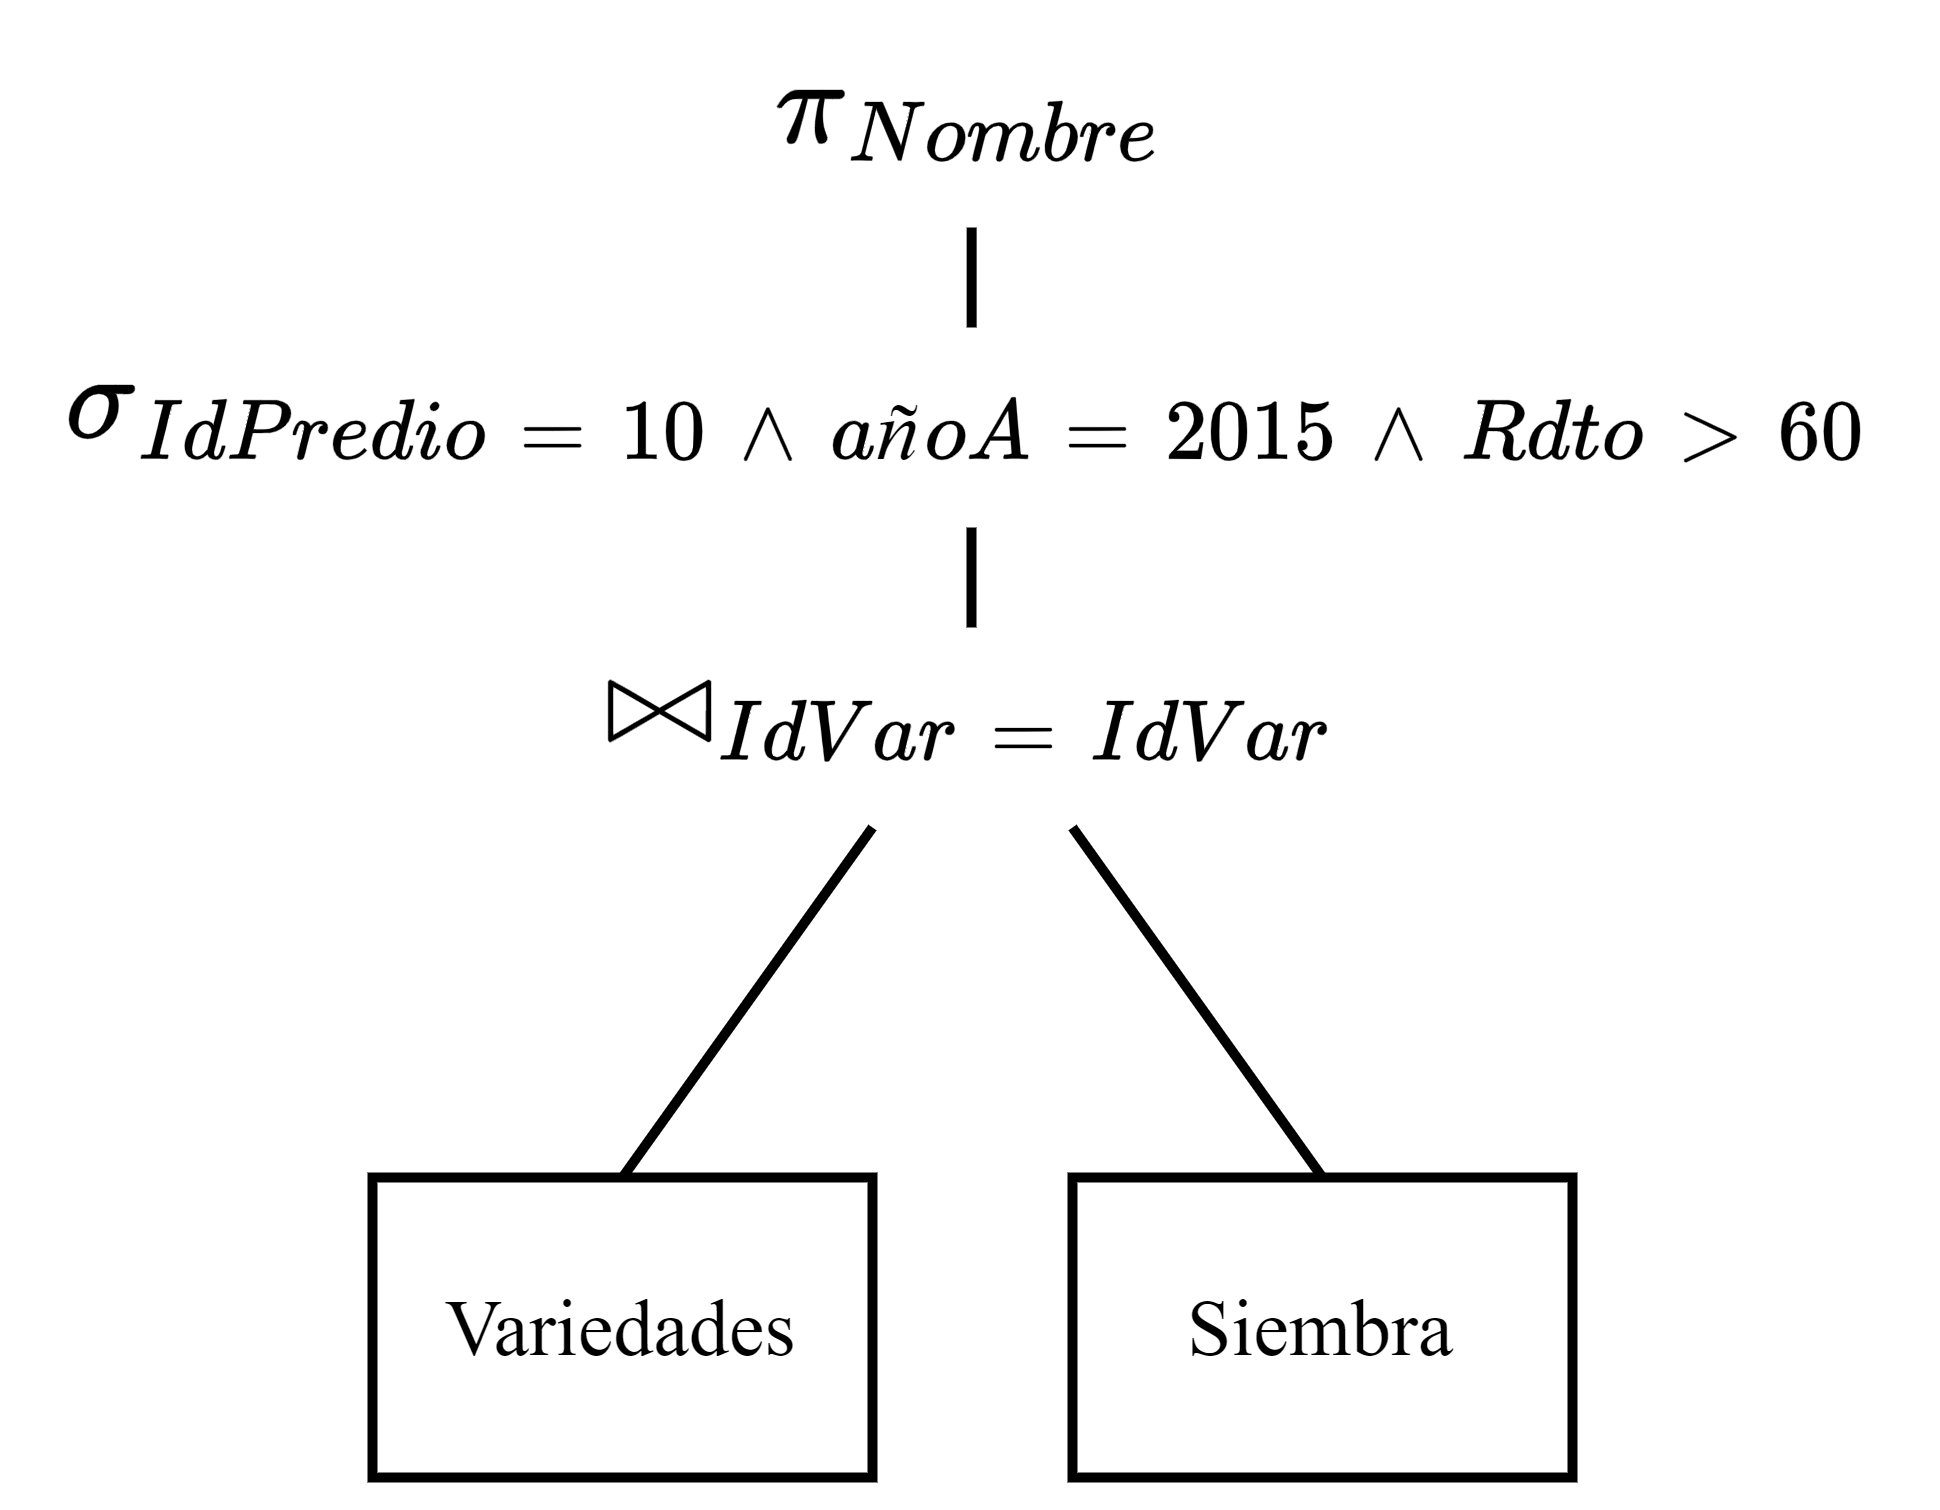
\includegraphics[width=0.5\textwidth]{img/E2-Paso4.png}
            \end{figure}

            \item Se bajan las demas selecciones a sus respectivas tablas.
            \begin{figure}[H]
                \centering
                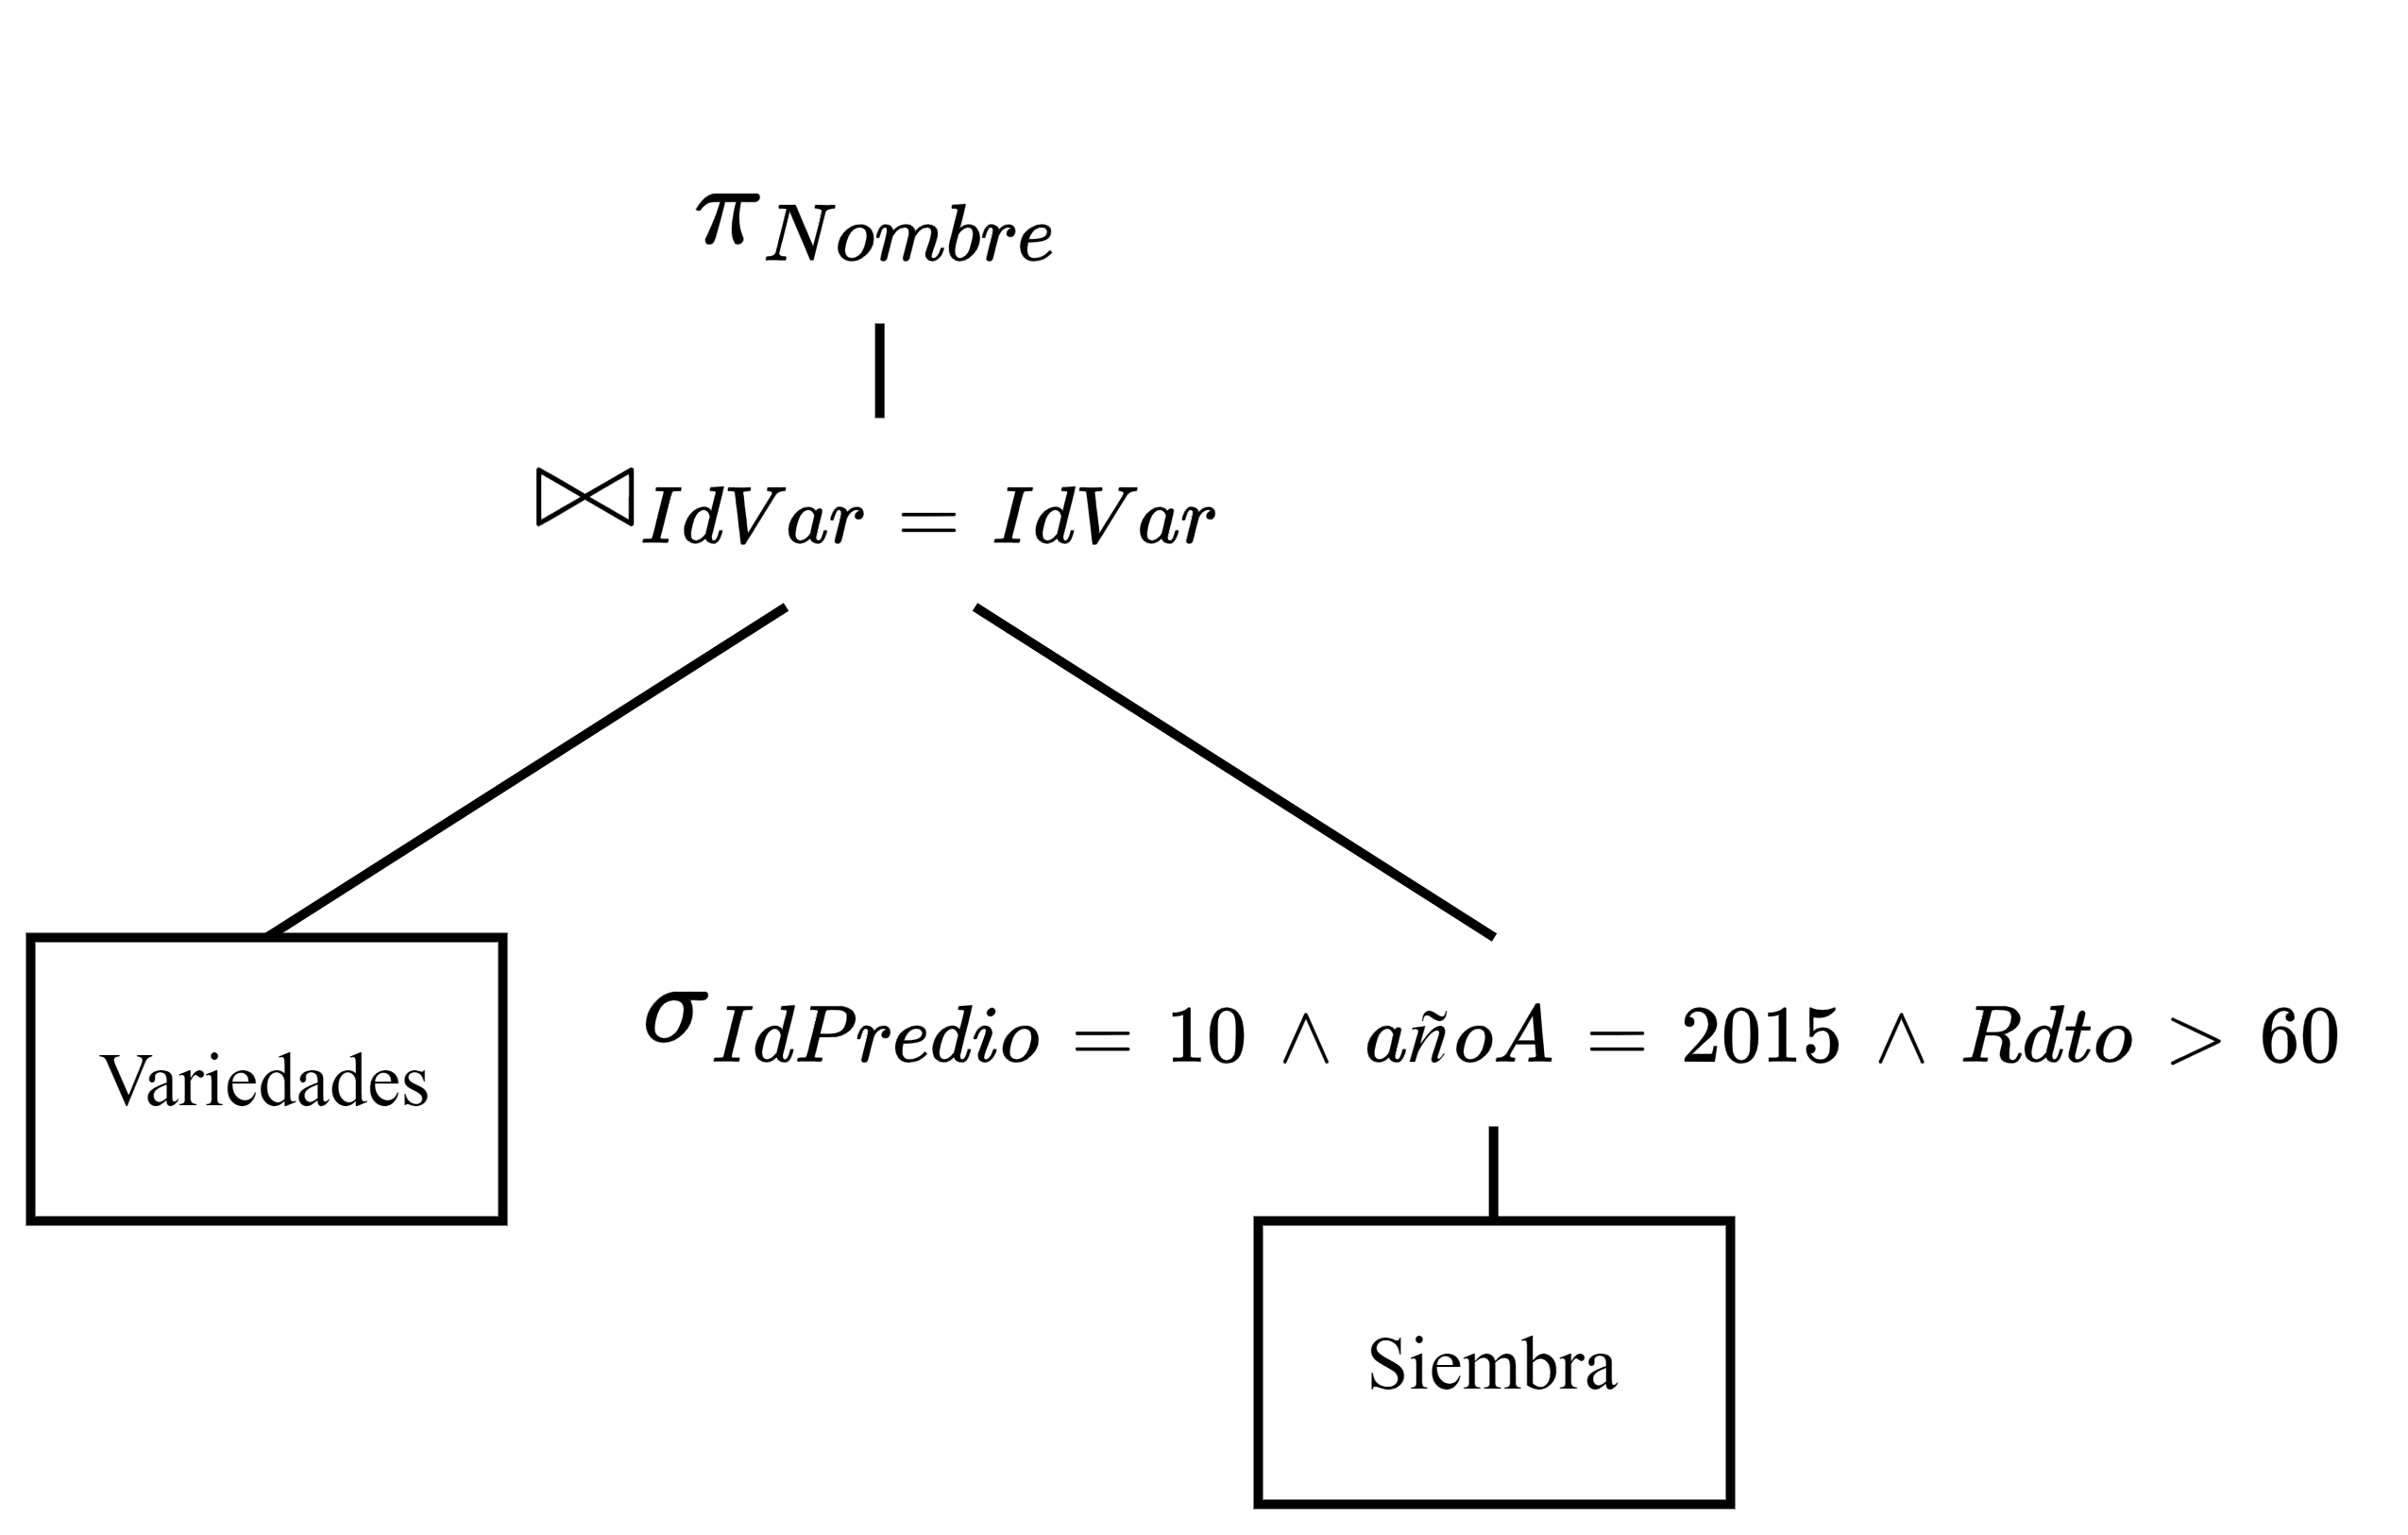
\includegraphics[width=0.6\textwidth]{img/E2-Paso5.png}
            \end{figure}

            \item Se proyecta solo lo necesario en las sub-tablas.
            \begin{figure}[H]
                \centering
                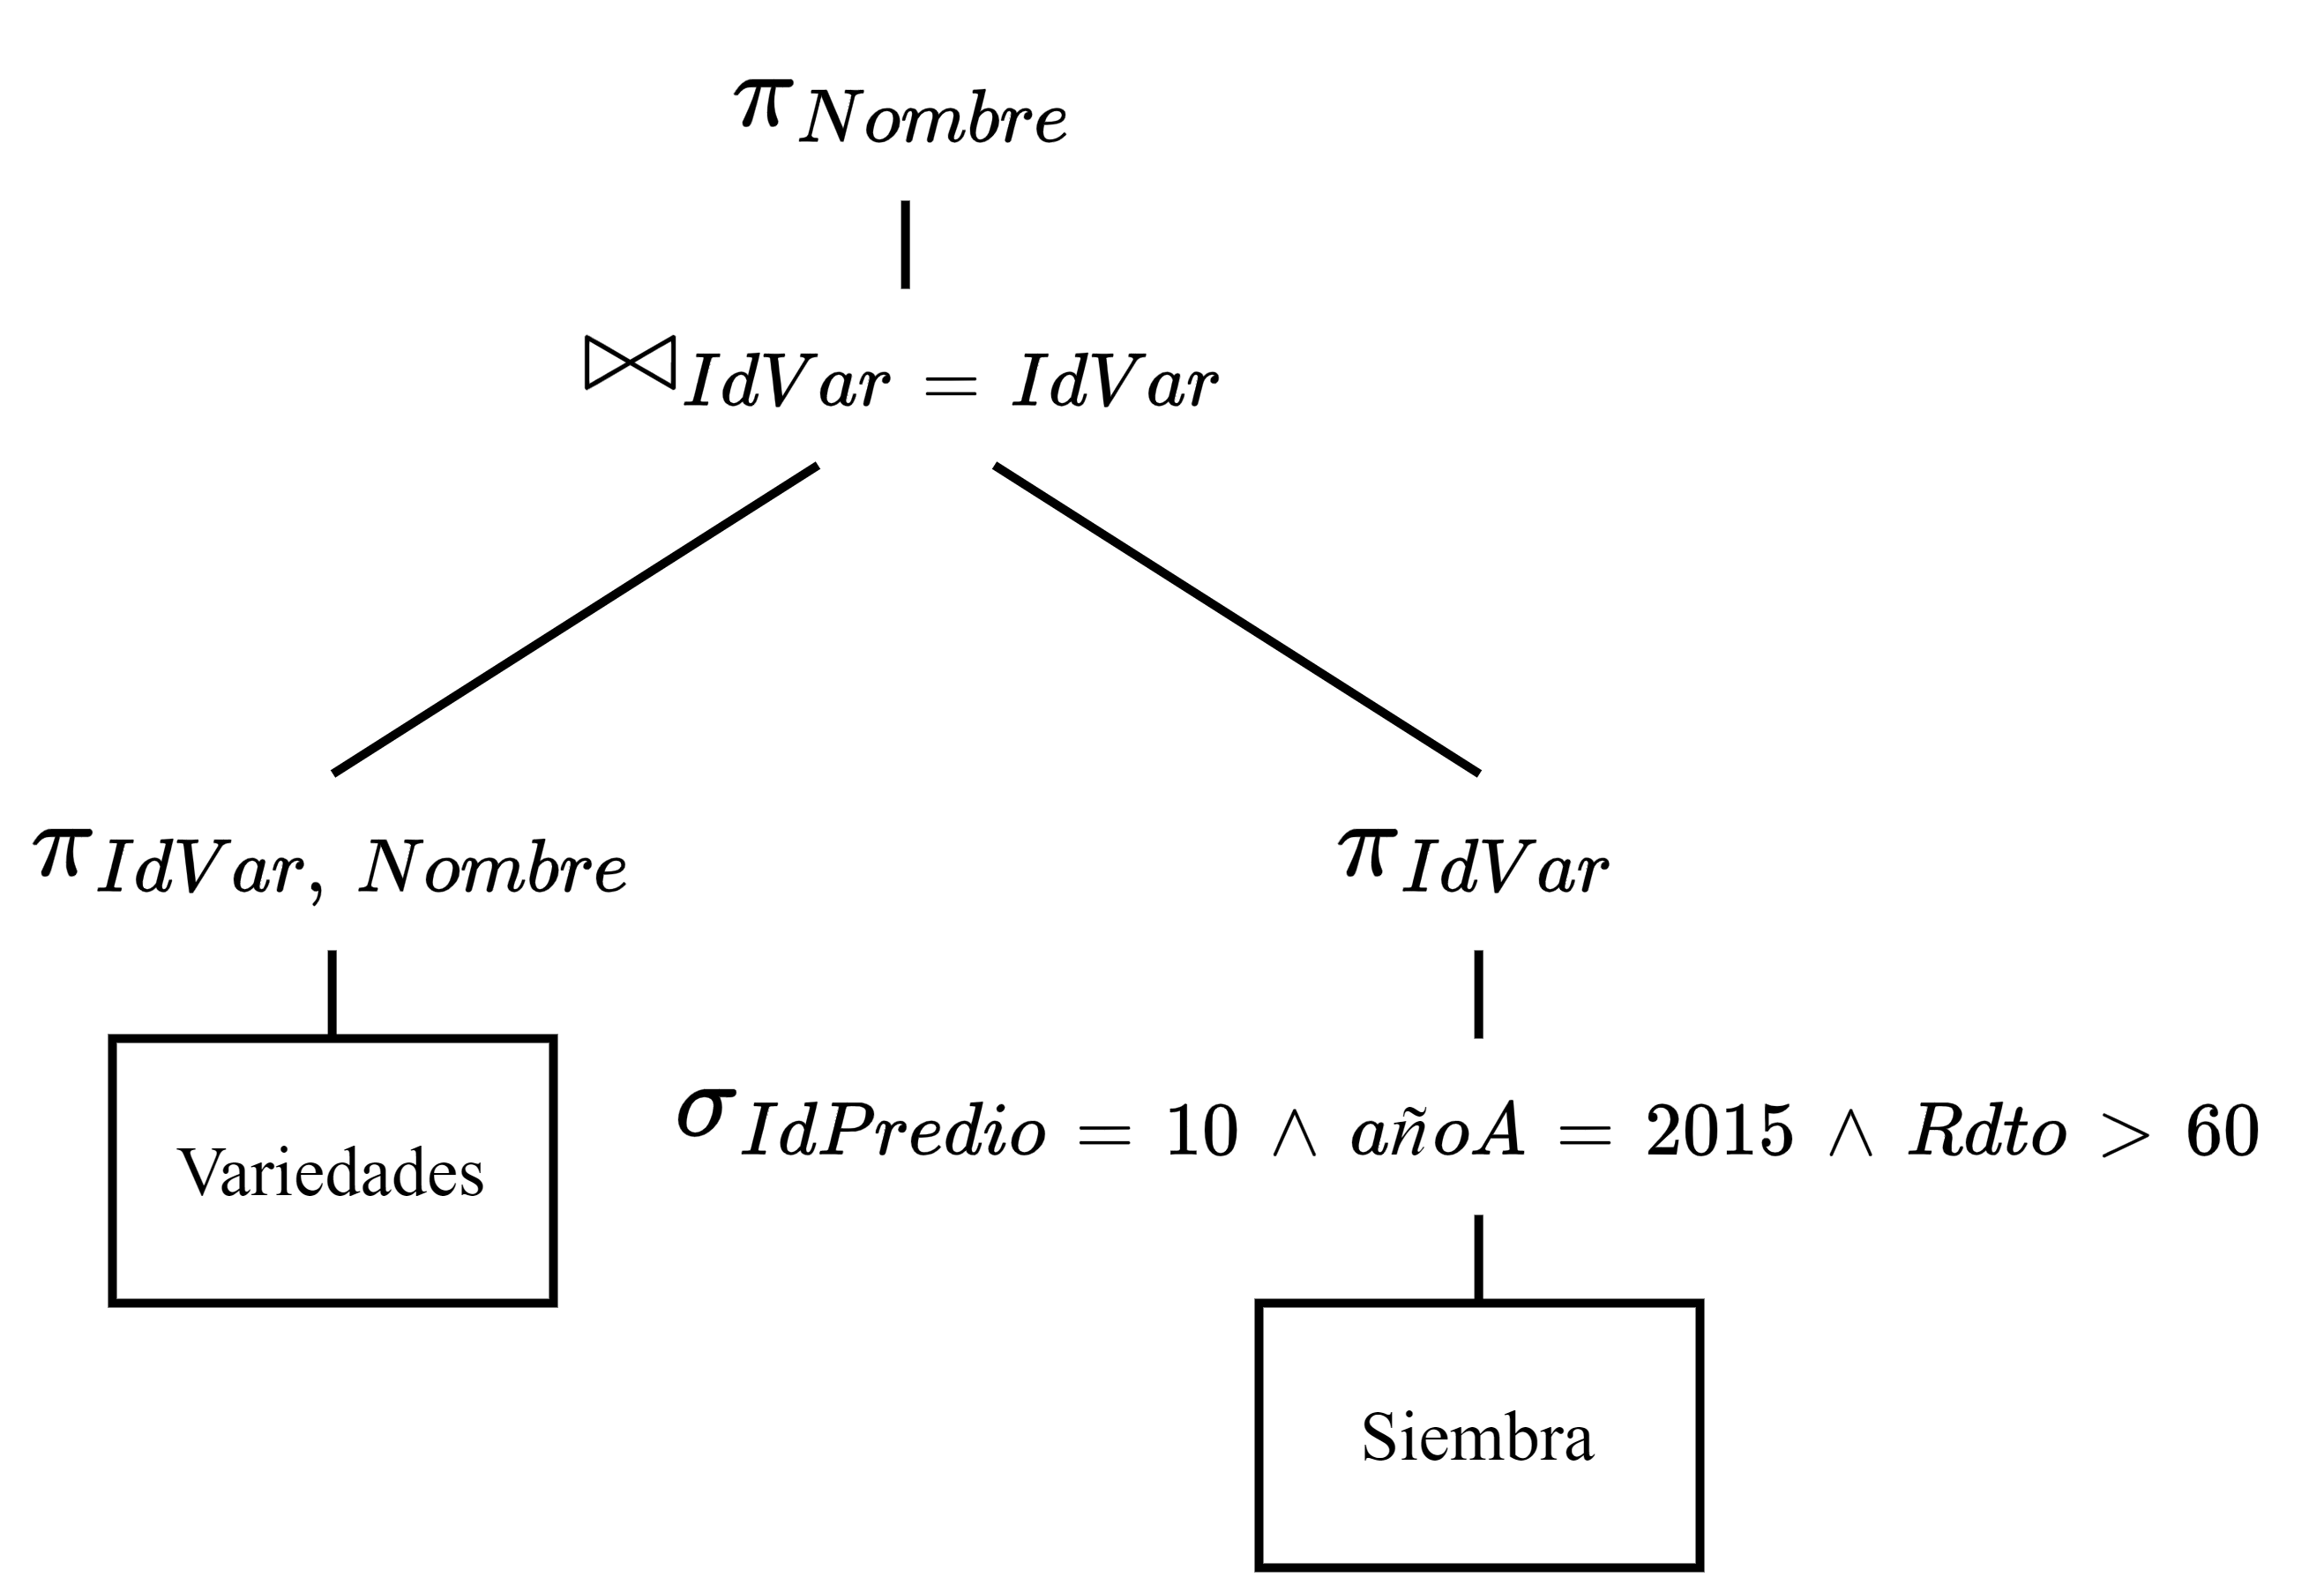
\includegraphics[width=0.6\textwidth]{img/E2-Paso6.png}
            \end{figure}
        \end{enumerate}
    \end{enumerate}

    \newpage
    \textbf{Para 3 y 4, calcular un orden/JOINS para R, S, T, U, usando programación dinámica (como visto en clases). Mostrar tabla inicial de costos, los calculos de cada etapa y árboles.}
    \item Suponer que tenemos las relaciones R(a, b), S(b, c), T(c, d) y U(d, e) con las siguientes características:
    \newparagraph
    \begin{minipage}{0.5\textwidth}
        \begin{itemize}
            \item T(R) = 300
            \item V(R, b) = 100
            \item T(S) = 200
            \item V(S, b) = 100
            \item V(S, c) = 20
        \end{itemize}
    \end{minipage}
    \hfill
    \begin{minipage}{0.5\textwidth}
        \begin{itemize}
            \item T(T) = 150
            \item V(T, c) = 20
            \item V(T, d) = 300
            \item T(U) = 500
            \item V(U, d) = 300
        \end{itemize}
    \end{minipage}
    \newparagraph
    \begin{center}
        \begin{tabular}{|c|c|c|c|}
            \hline
            R & S & T & U \\
            \hline
            T(R) = 300 & T(S) = 200 & T(T) = 150 & T(U) = 500 \\
            V(R, b) = 100 & V(S, b) = 100 & & \\
            & V(S, c) = 20 & V(T, c) = 20 & \\
            & & V(T, d) = 300 & V(U, d) = 300 \\
            \hline
        \end{tabular}
    \end{center}
    \newparagraph

    \textbf{Paso a paso:}
    \begin{enumerate}[label=\arabic*)]
        \item Costos simples.
        \begin{center}
            \begin{tabular}{|r|c|c|c|c|}
                \hline
                & R & S & T & U \\
                \hline
                \textbf{Tamaño} & 300 & 200 & 150 & 500 \\
                \hline
                \textbf{Costo}  & 0 & 0 & 0 & 0 \\
                \hline
                \textbf{Mejor Plan} & R & S & T & U \\
                \hline
            \end{tabular}
        \end{center}
        \newparagraph

        \item Calculo simples.
        \newparagraph
        \begin{minipage}{0.5\textwidth}
            \begin{itemize}
                \item $T(R) = 300$
                \item $T(S) = 200$
            \end{itemize}
        \end{minipage}
        \hfill
        \begin{minipage}{0.5\textwidth}
            \begin{itemize}
                \item $T(T) = 150$ *
                \item $T(U) = 500$
            \end{itemize}
        \end{minipage}
        \newparagraph

        \item Costo pares.
        \begin{center}
            \begin{tabular}{|r|c|c|c|c|c|c|c|}
                \hline
                & $\{R, \; S\}$ & $\{R, \; T\}$ & $\{R, \; U\}$ & $\{S, \; T\}$ & $\{S, \; U\}$ & $\{T, \; U\}$ \\
                \hline
                \textbf{Tamaño} & 600 & 45000 & 150000 & 1500 & 100000 & 250 \\
                \hline
                \textbf{Costo}  & 0 & 0 & 0 & 0 & 0 & 0 \\
                \hline
                \textbf{Mejor Plan} & $R \Join S$ & $R \Join T$ & $R \Join U$ & $S \Join T$ & $S \Join U$ & $T \Join U$ \\
                \hline
            \end{tabular}
        \end{center}
        \newparagraph

        \item Calculo pares.
        \begin{itemize}
            \item $T(R \Join S) =  \displaystyle\frac{T(R) \cdot T(S)}{\text{max}\{V(R,b), \; V(S,b)\}} = \frac{300 \cdot 200}{\text{max} \{100, 100\}} = \frac{60000}{100} = \colorbox{gray!20}{600}$ \newparagraph
            \item $T(R \Join T) =  \displaystyle\frac{T(R) \cdot T(T)}{\text{max}\{V(R,-), \; V(T,-)\}} = 300 \cdot 150 = \colorbox{gray!20}{45000}$ \newparagraph
            \item $T(R \Join U) =  \displaystyle\frac{T(R) \cdot T(U)}{\text{max}\{V(R,-), \; V(U,-)\}} = 300 \cdot 500 = \colorbox{gray!20}{150000}$ \newparagraph
            \item $T(S \Join T) =  \displaystyle\frac{T(S) \cdot T(T)}{\text{max}\{V(S,c), \; V(T,c)\}} = \frac{200 \cdot 150}{\text{max} \{20, 20\}} = \frac{30000}{20} = \colorbox{gray!20}{1500}$ \newparagraph
            \item $T(S \Join U) =  \displaystyle\frac{T(S) \cdot T(U)}{\text{max}\{V(S,-), \; V(U,-)\}} = 200 \cdot 500 = \colorbox{gray!20}{100000}$ \newparagraph
            \item $T(T \Join U) =  \displaystyle\frac{T(T) \cdot T(U)}{\text{max}\{V(T,d), \; V(U,d)\}} = \frac{150 \cdot 500}{\text{max} \{300, 300\}} = \frac{75000}{300} = \colorbox{gray!20}{250}$ \newparagraph
        \end{itemize}

        \item Costo tripletas.
        \begin{center}
            \begin{tabular}{|r|c|c|c|c|}
                \hline
                & $\{R, \; S, \; T\}$ & $\{R, \; S, \; U\}$ & $\{R, \; T, \; U\}$ & $\{S, \; T, \; U\}$ \\
                \hline
                \textbf{Tamaño} & 4500 & 300000 & 75000 & 2500 \\
                \hline
                \textbf{Costo}  & 600 & 600 & 250 & 250 \\
                \hline
                \textbf{Mejor Plan} & $(R \Join S) \Join T$ & $(R \Join S) \Join U$ & $(T \Join U) \Join R$ & $(T \Join U) \Join S$ \\
                \hline
            \end{tabular}
        \end{center}
        \newparagraph

        \item Calculo tripletas.
        \begin{itemize}
            \item Para $\{R, \; S, \; T\}$
            \begin{itemize}
                \item $T(R \Join S) = \colorbox{gray!20}{600}$ *
                \item $T(R \Join T) = 45000$
                \item $T(S \Join T) = 1500$
            \end{itemize}
            \begin{align*}
                T((R \Join S) \Join T) &= \displaystyle\frac{T(R \Join S) \cdot T(T)}{\text{max}\{V((R \Join S), c), \; V(T,c)\}} \\
                &= \frac{600 \cdot 150}{\text{max}\{20, 20\}} = \frac{90000}{20} = \colorbox{gray!20}{4500}
            \end{align*}
            \newparagraph

            \newpage
            \item Para $\{R, \; S, \; U\}$
            \begin{itemize}
                \item $T(R \Join S) = \colorbox{gray!20}{600}$ *
                \item $T(R \Join U) = 150000$
                \item $T(S \Join U) = 100000$
            \end{itemize}
            \begin{align*}
                T((R \Join S) \Join U) &= \displaystyle\frac{T(R \Join S) \cdot T(U)}{\text{max}\{V(R\Join S,-), \; V(U,-)\}} \\
                &= 600 \cdot 500 = \colorbox{gray!20}{300000}
            \end{align*}
            \newparagraph

            \item Para $\{R, \; T, \; U\}$
            \begin{itemize}
                \item $T(R \Join T) = 45000$
                \item $T(R \Join U) = 150000$
                \item $T(T \Join U) = \colorbox{gray!20}{250}$ *
            \end{itemize}
            \begin{align*}
                T((T \Join U) \Join R) &= \displaystyle\frac{T(T \Join U) \cdot T(R)}{\text{max}\{V(T \Join U,-), \; V(R,-)\}} \\
                &= 250 \cdot 300 = \colorbox{gray!20}{75000}
            \end{align*}
            \newparagraph

            \item Para $\{S, \; T, \; U\}$
            \begin{itemize}
                \item $T(S \Join T) = 1500$
                \item $T(S \Join U) = 100000$
                \item $T(T \Join U) = \colorbox{gray!20}{250}$ *
            \end{itemize}
            \begin{align*}
                T((T \Join U) \Join S) &= \displaystyle\frac{T(T \Join U) \cdot T(S)}{\text{max}\{V((T \Join U),c), \; V(S,c)\}} \\
                &= \frac{250 \cdot 200}{\text{max}\{20, 20\}} = \frac{50000}{20} = \colorbox{gray!20}{2500}
            \end{align*}
            \newparagraph
        \end{itemize}
        
        \item Arboles.
        \begin{itemize}
            \item Para $\{R, \; S, \; T\}$
            \begin{figure}[H]
                \centering
                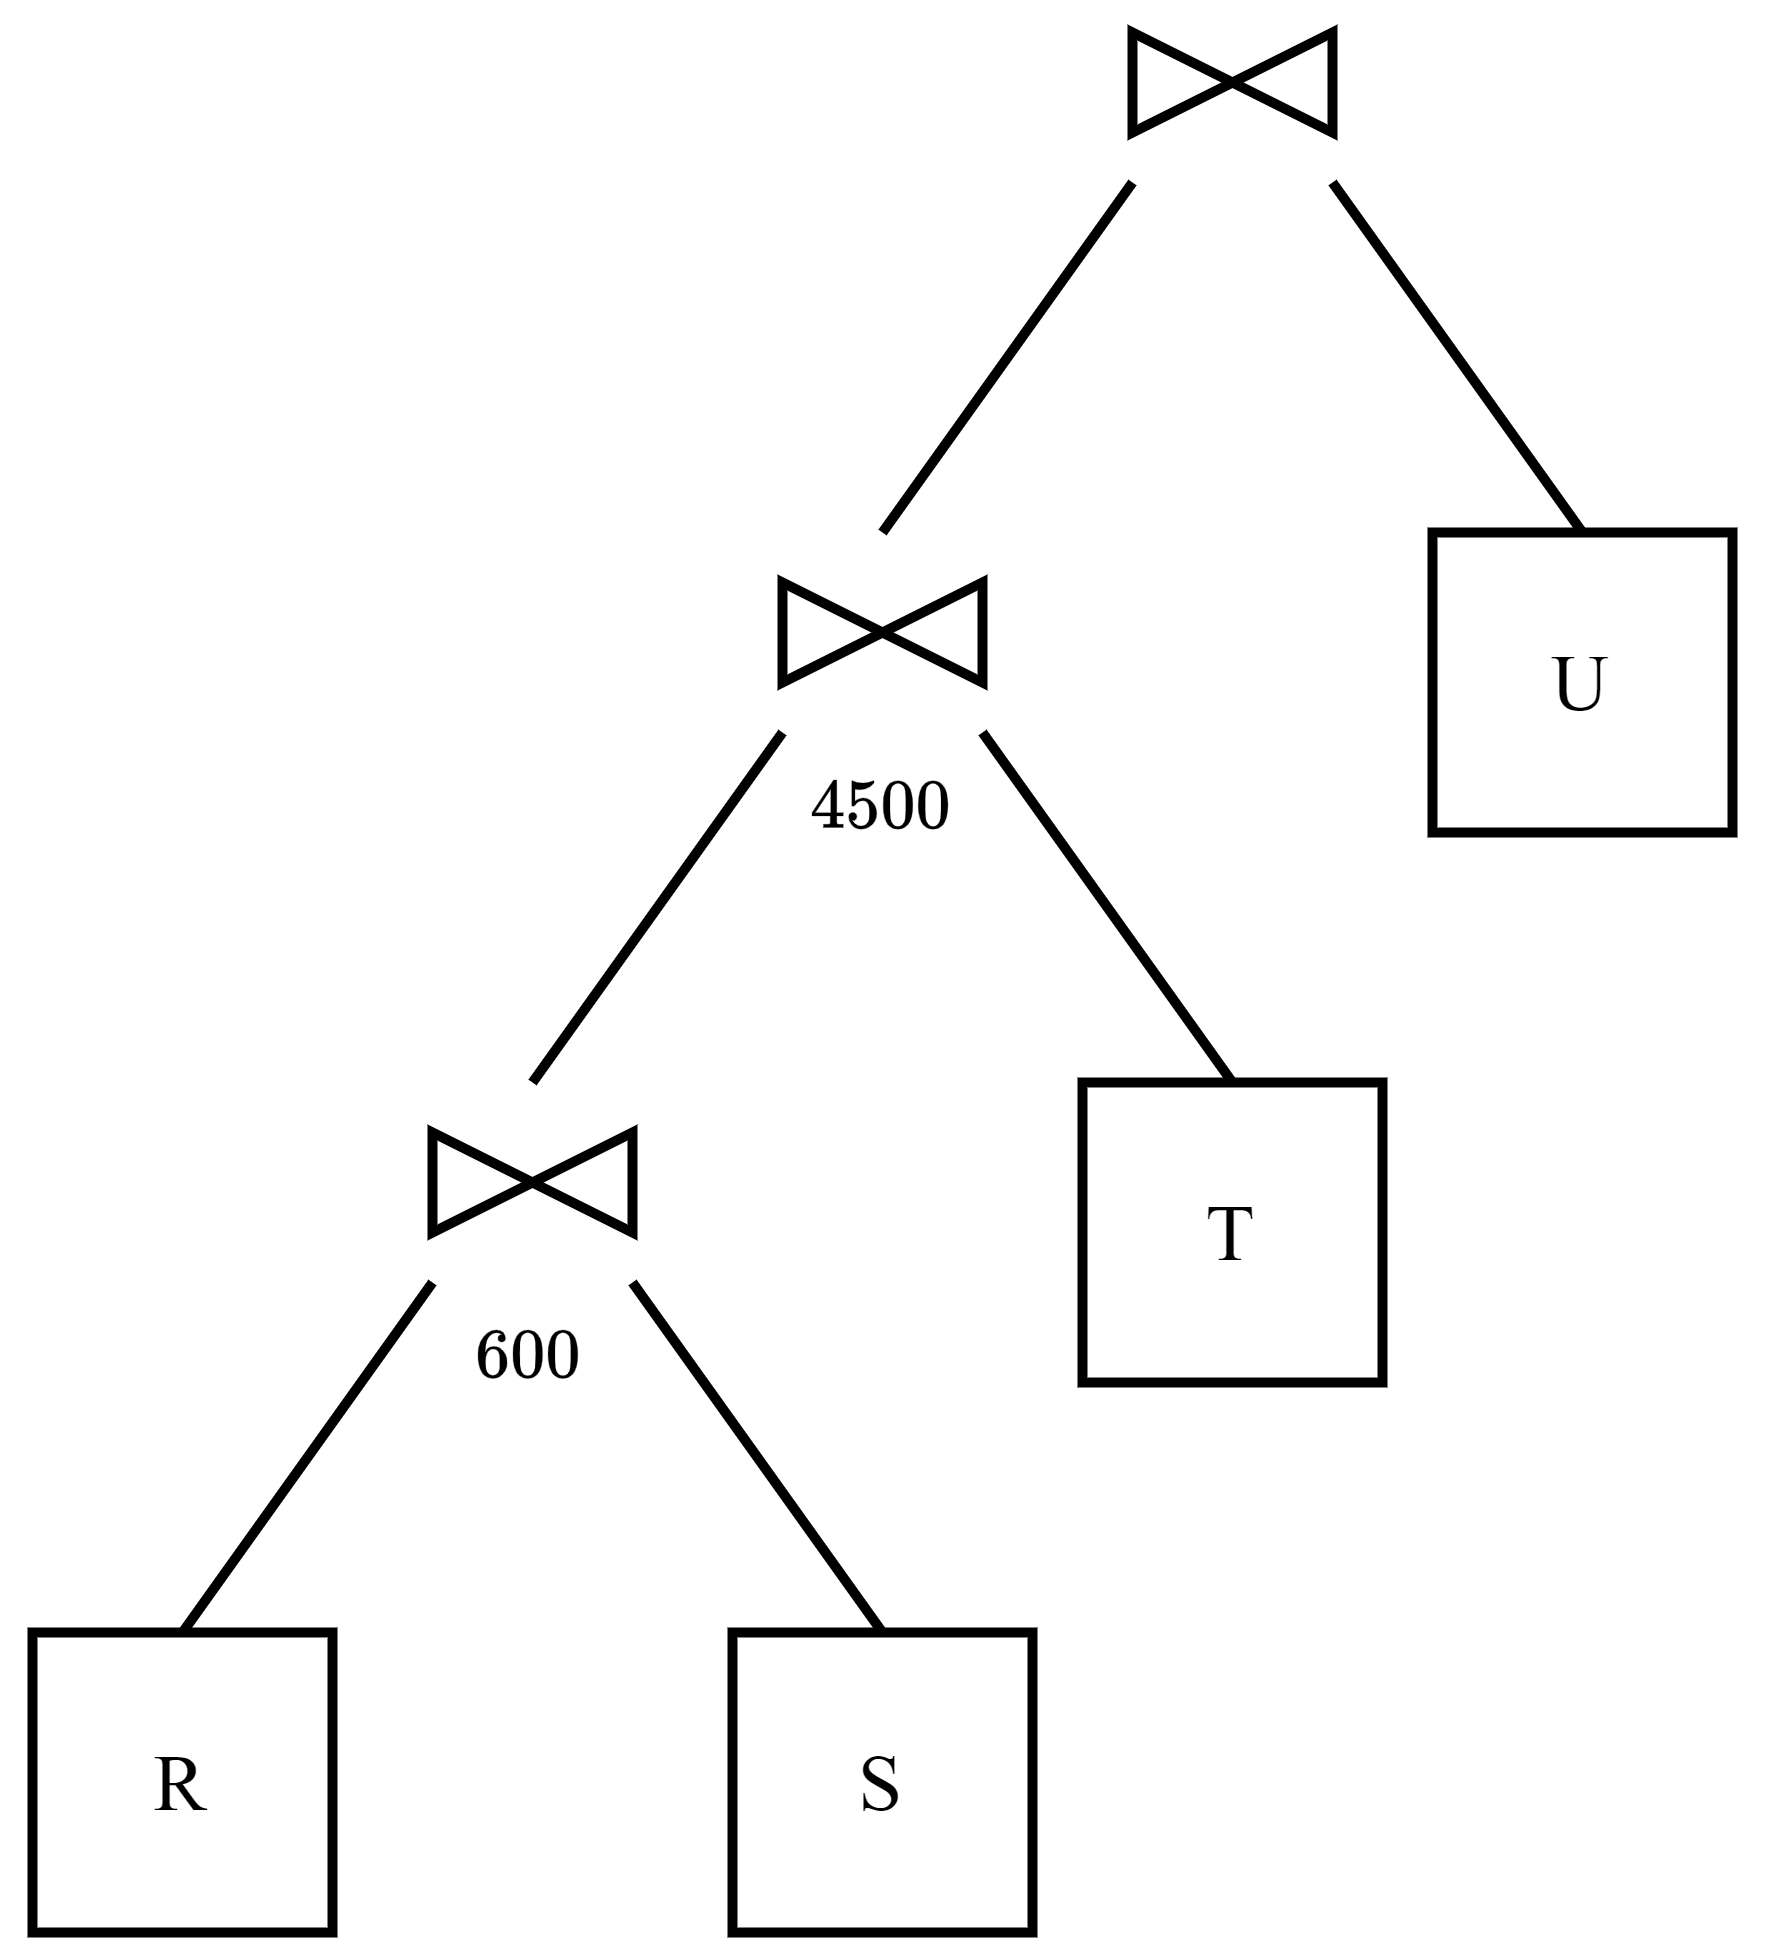
\includegraphics[width=0.35\textwidth]{img/E3-A1.png}
            \end{figure}

            \newpage
            \item Para $\{R, \; S, \; U\}$
            \begin{figure}[H]
                \centering
                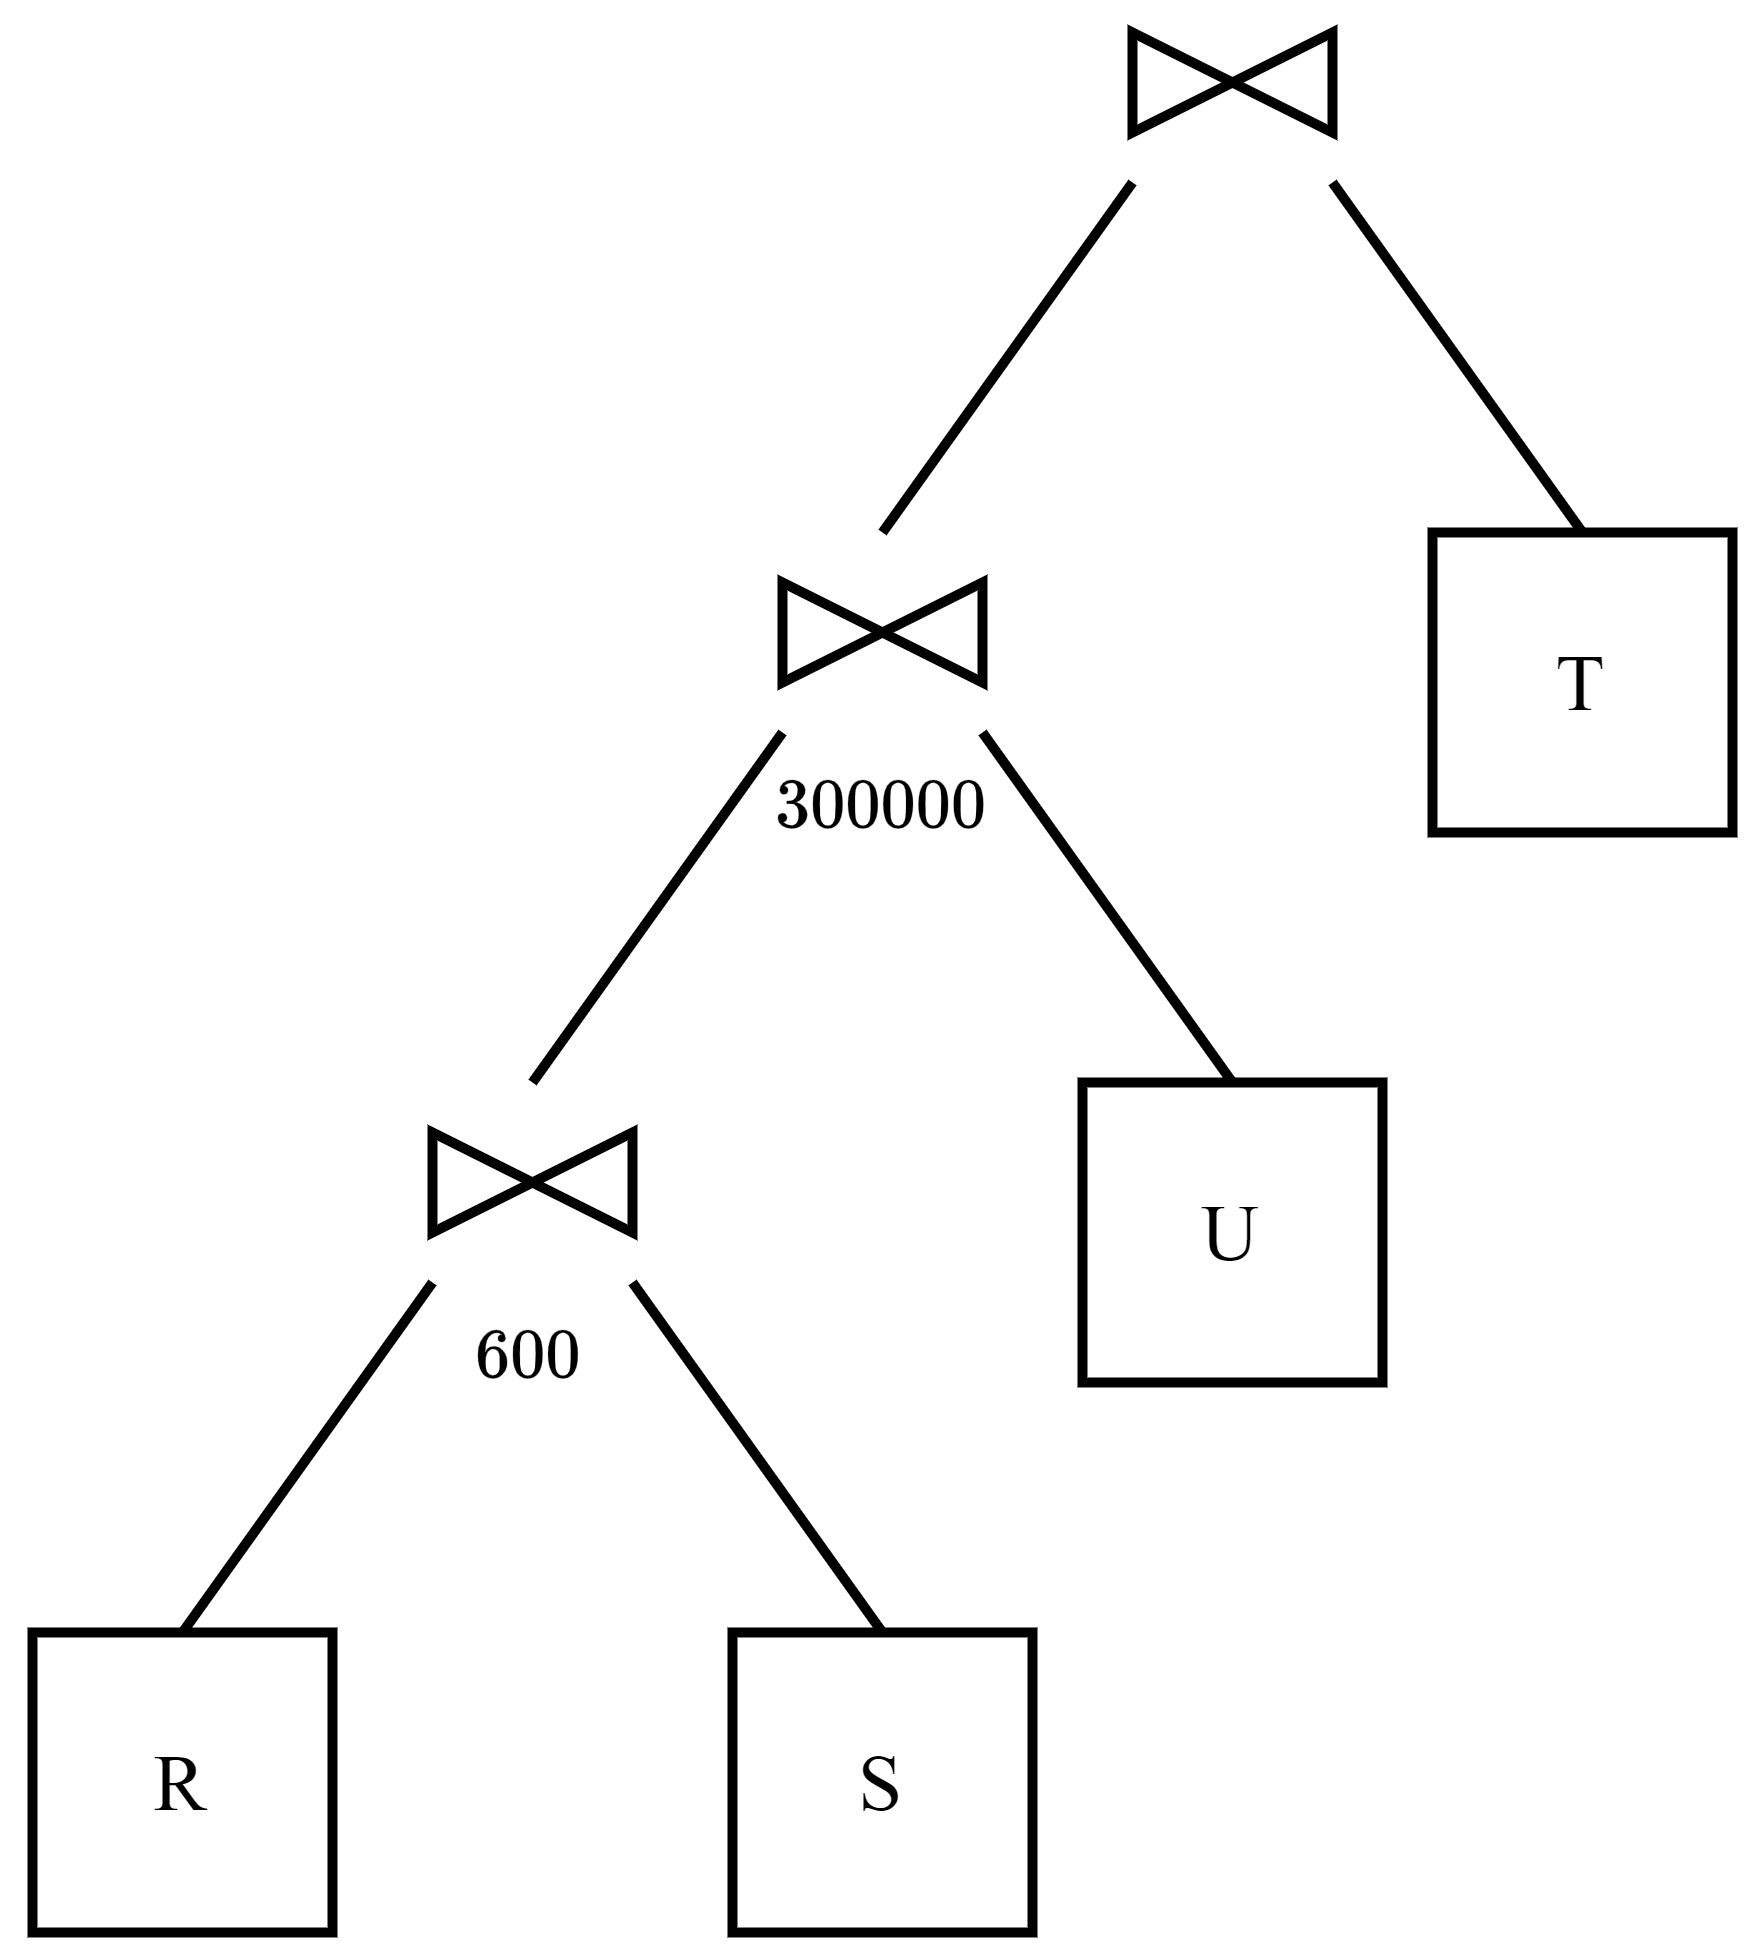
\includegraphics[width=0.35\textwidth]{img/E3-A2.png}
            \end{figure}

            \item Para $\{R, \; T, \; U\}$
            \begin{figure}[H]
                \centering
                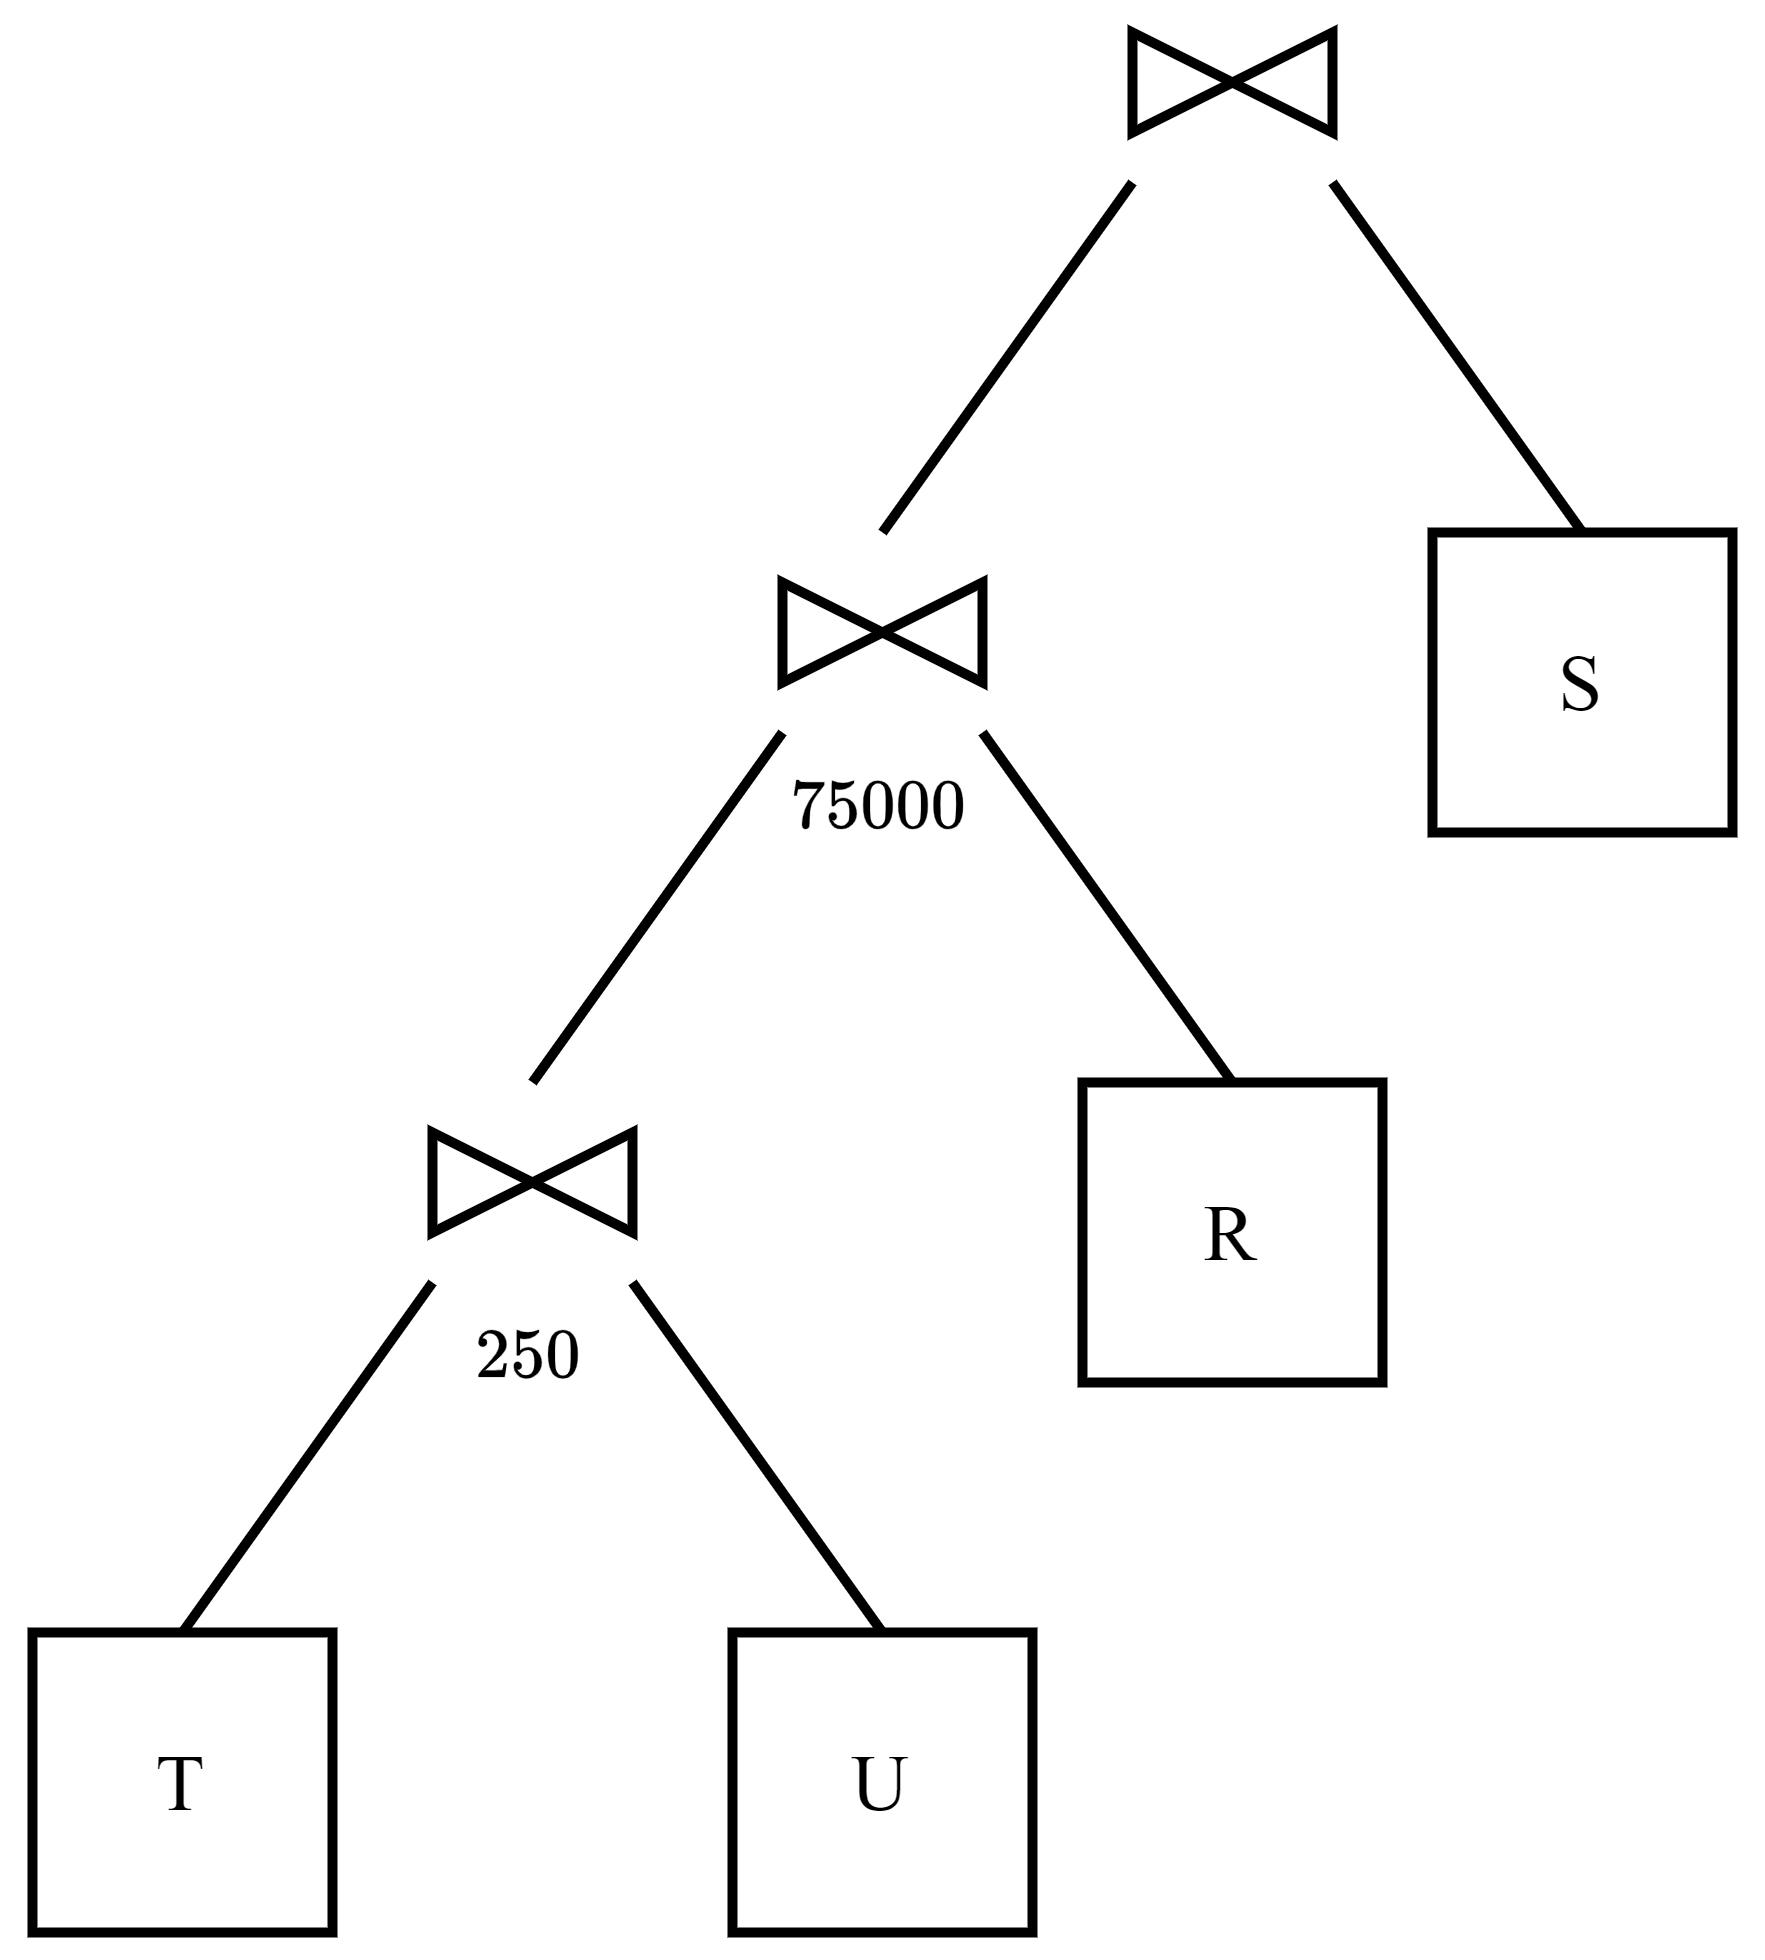
\includegraphics[width=0.35\textwidth]{img/E3-A3.png}
            \end{figure}

            \item Para $\{S, \; T, \; U\}$
            \begin{figure}[H]
                \centering
                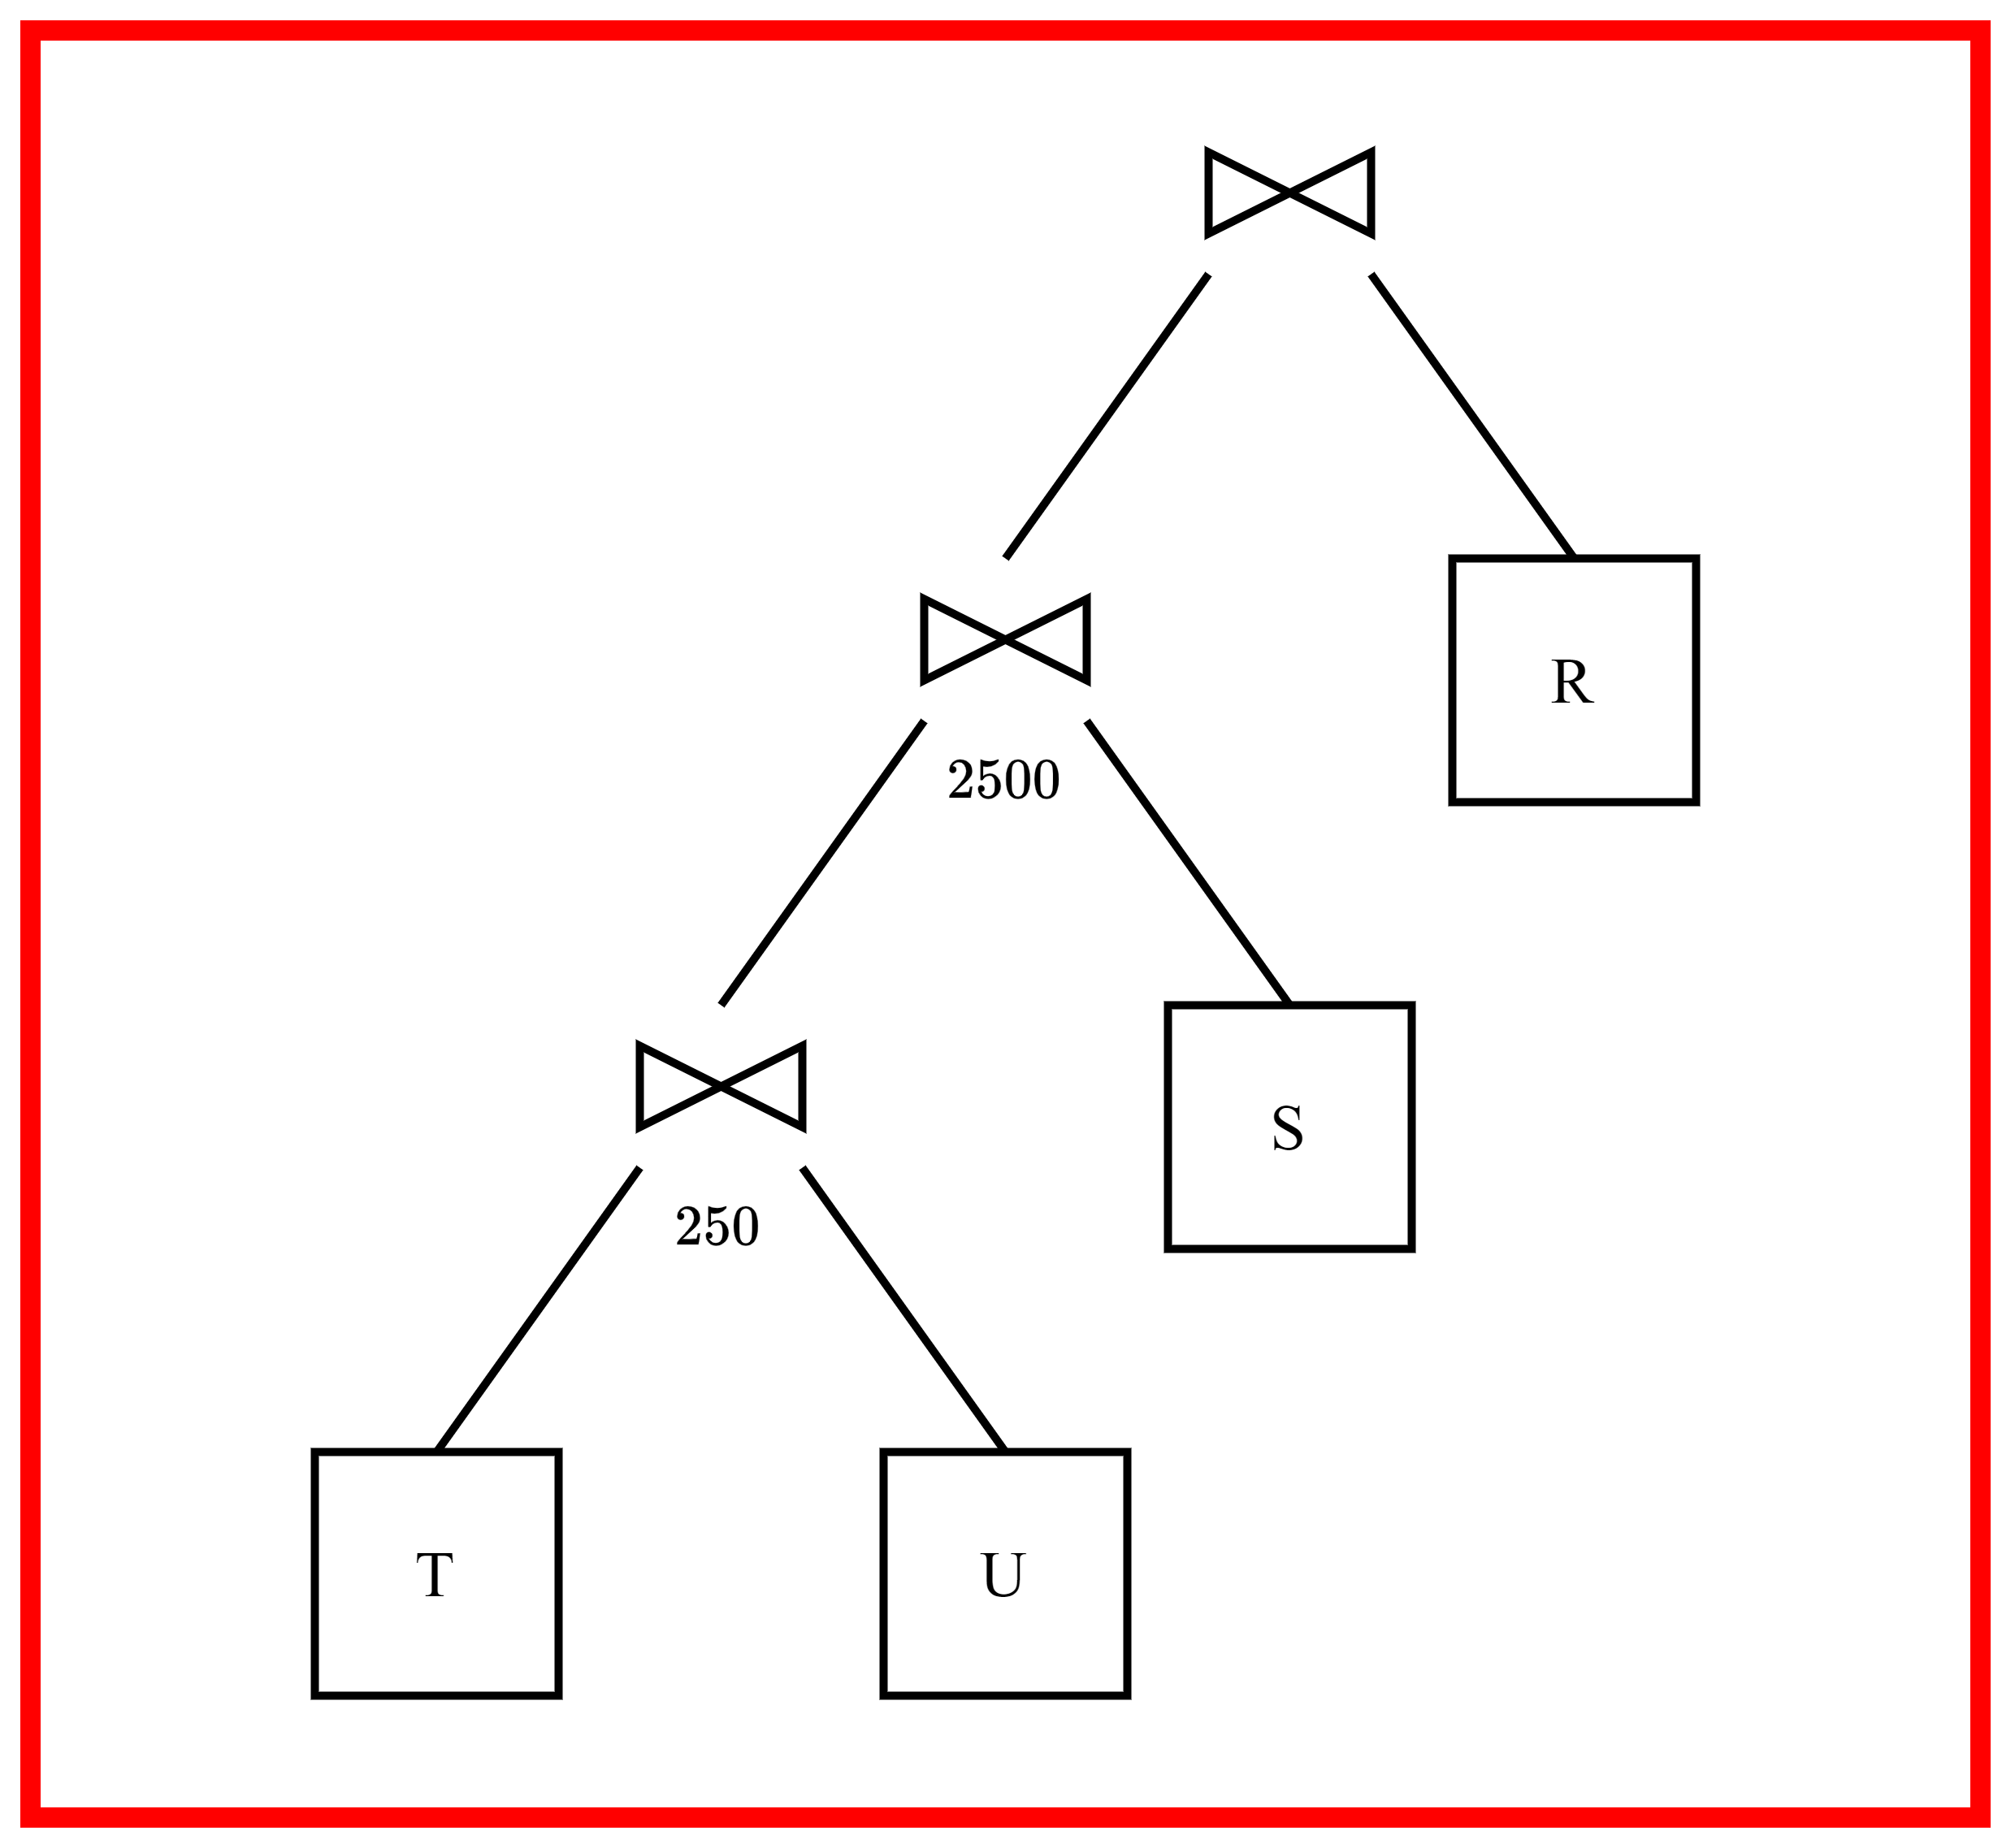
\includegraphics[width=0.5\textwidth]{img/E3-A4.png}
            \end{figure}
        \end{itemize}

        \newpage
        \textbf{Agrupando tenemos que el costo es:}
        \begin{itemize}
            \item $(((R \Join S) \Join T) \Join U) = 600 + 4500 = 5100$
            \item $(((R \Join S) \Join U) \Join T) = 600 + 300000 = 300600$
            \item $(((T \Join U) \Join R) \Join S) = 250 + 75000 = 75250$
            \item $(((T \Join U) \Join S) \Join R) = 2500 + 250 = 2750$ *
        \end{itemize}

        \begin{equation*}
            \therefore \quad \text{El mejor plan es: } (((T \Join U) \Join S) \Join R)
        \end{equation*}
        \newparagraph

        \item Realizando el árbol balanceado.
        \begin{itemize}
            \item Para $(R \Join S) \Join (T \Join U)$
            \begin{figure}[H]
                \centering
                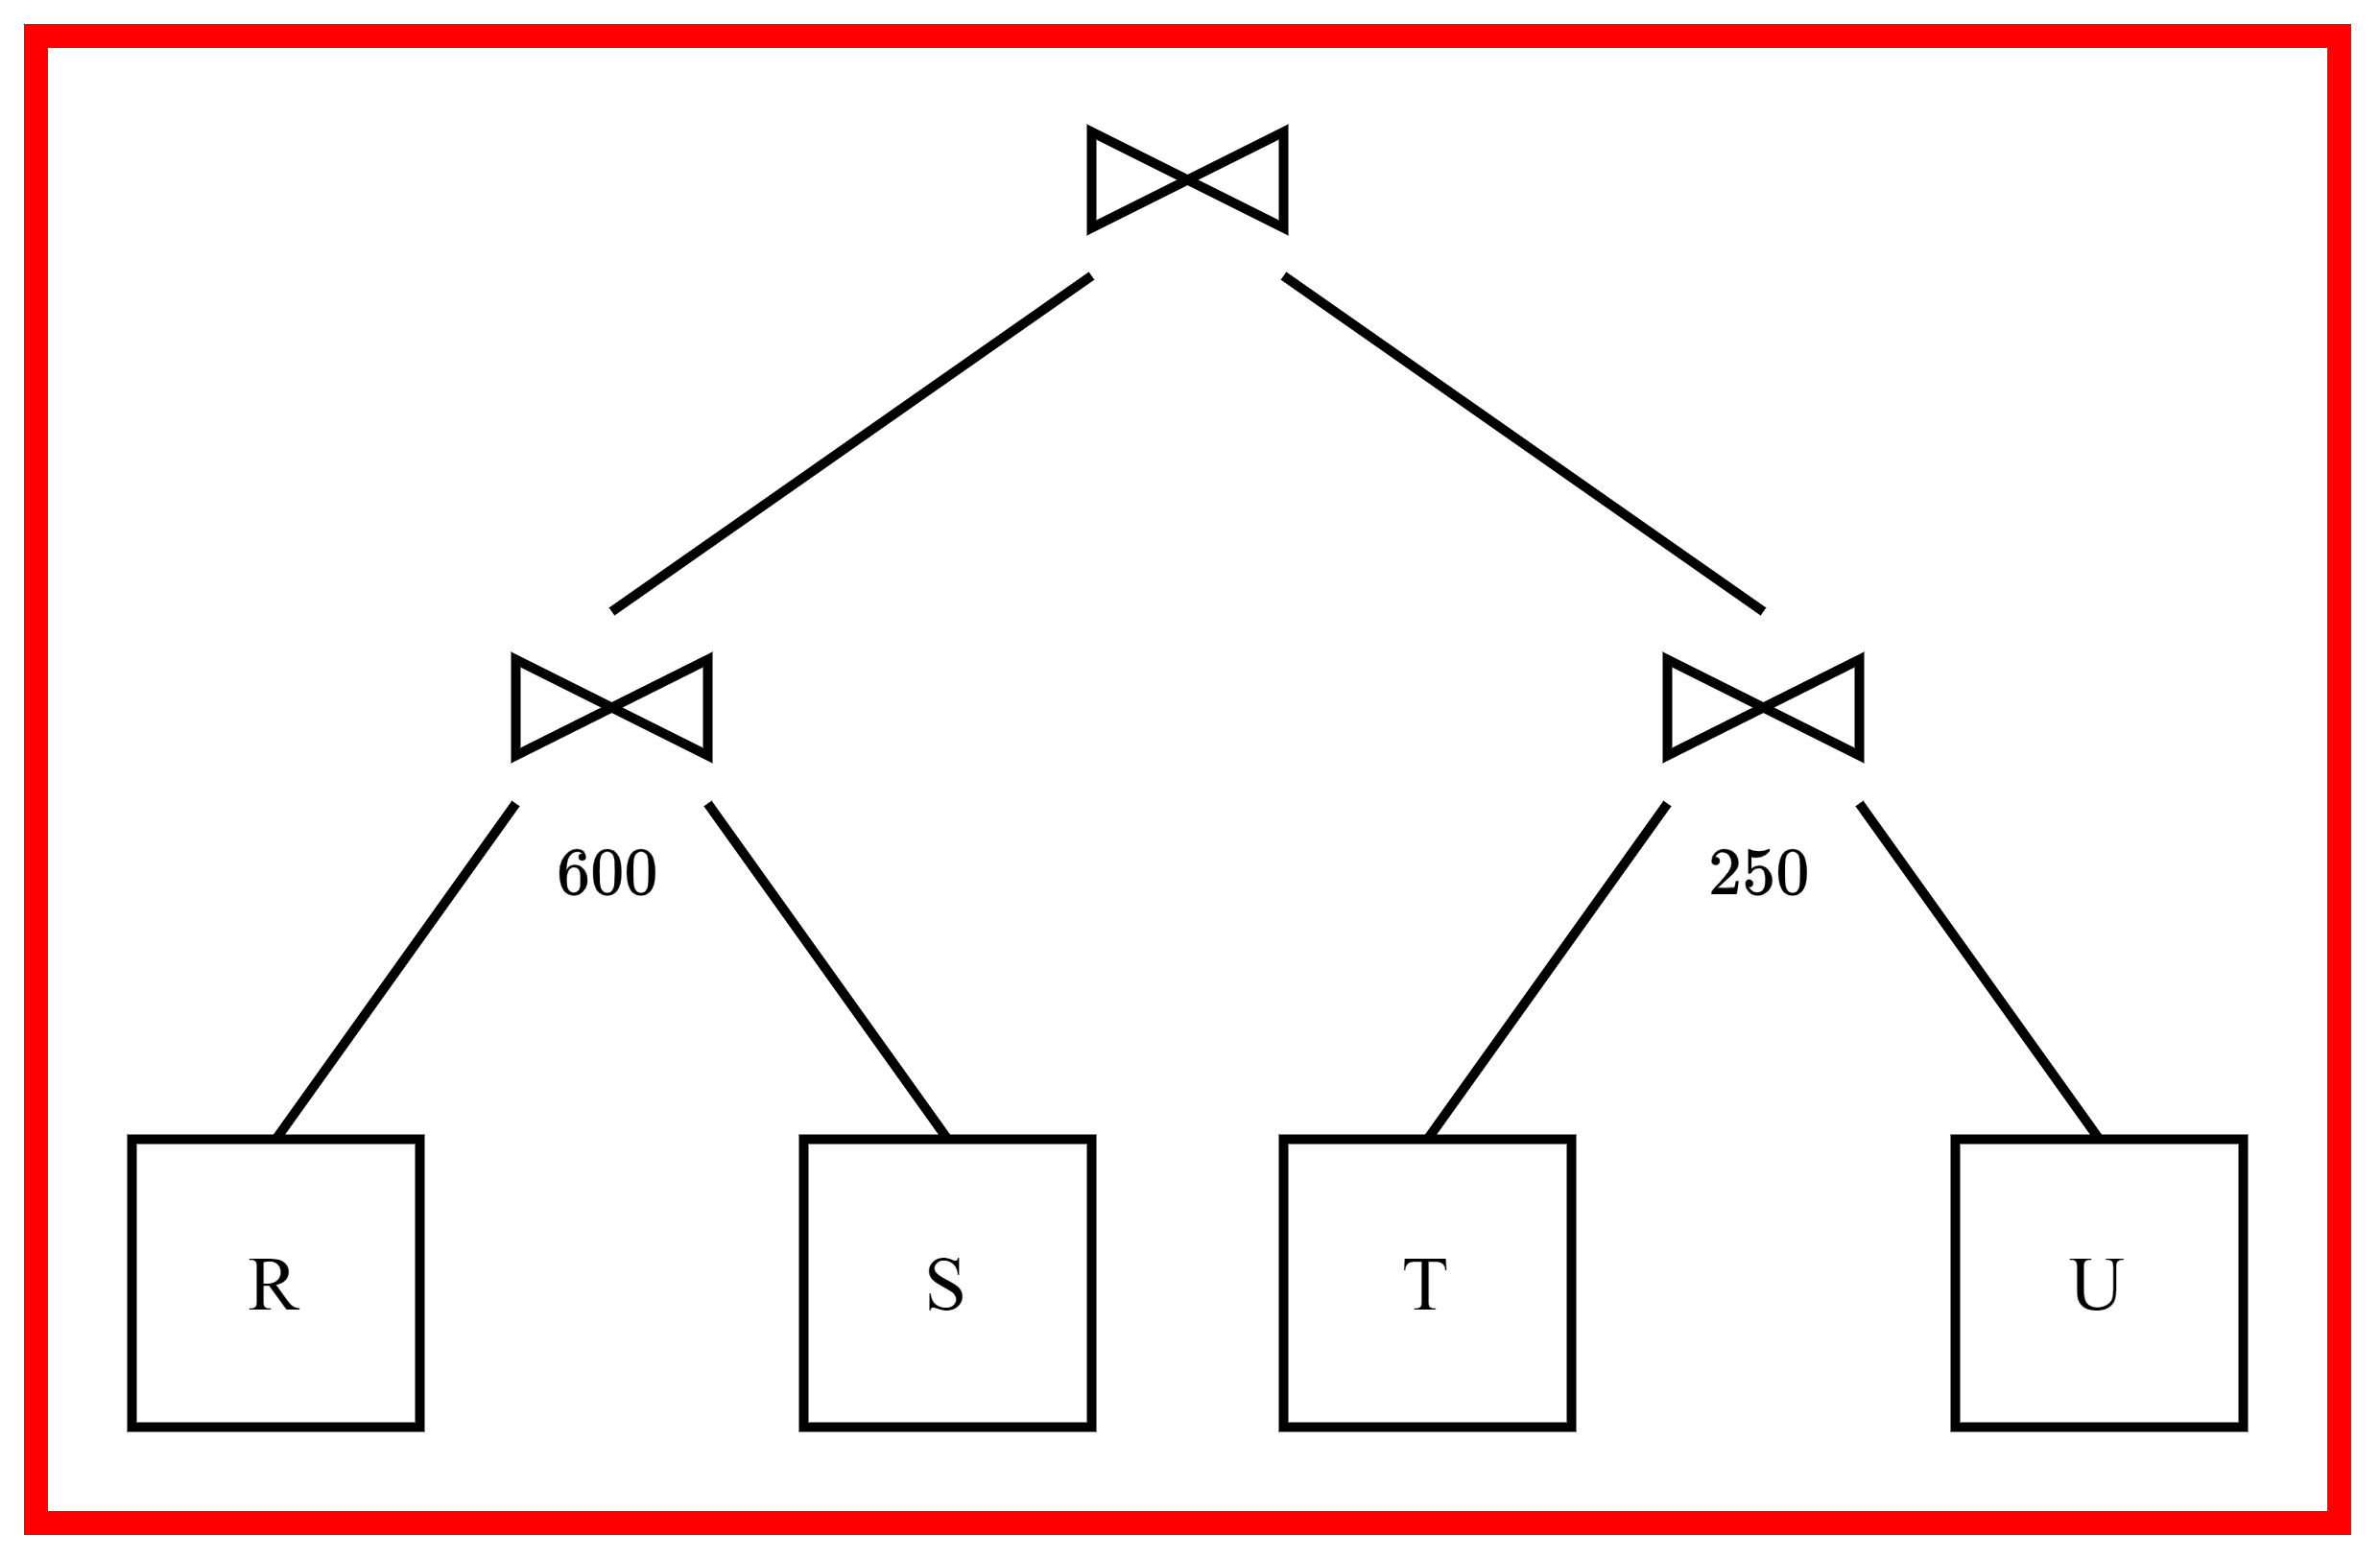
\includegraphics[width=0.55\textwidth]{img/E3-AB1.png}
            \end{figure}

            \item Para $(R \Join T) \Join (S \Join U)$
            \begin{figure}[H]
                \centering
                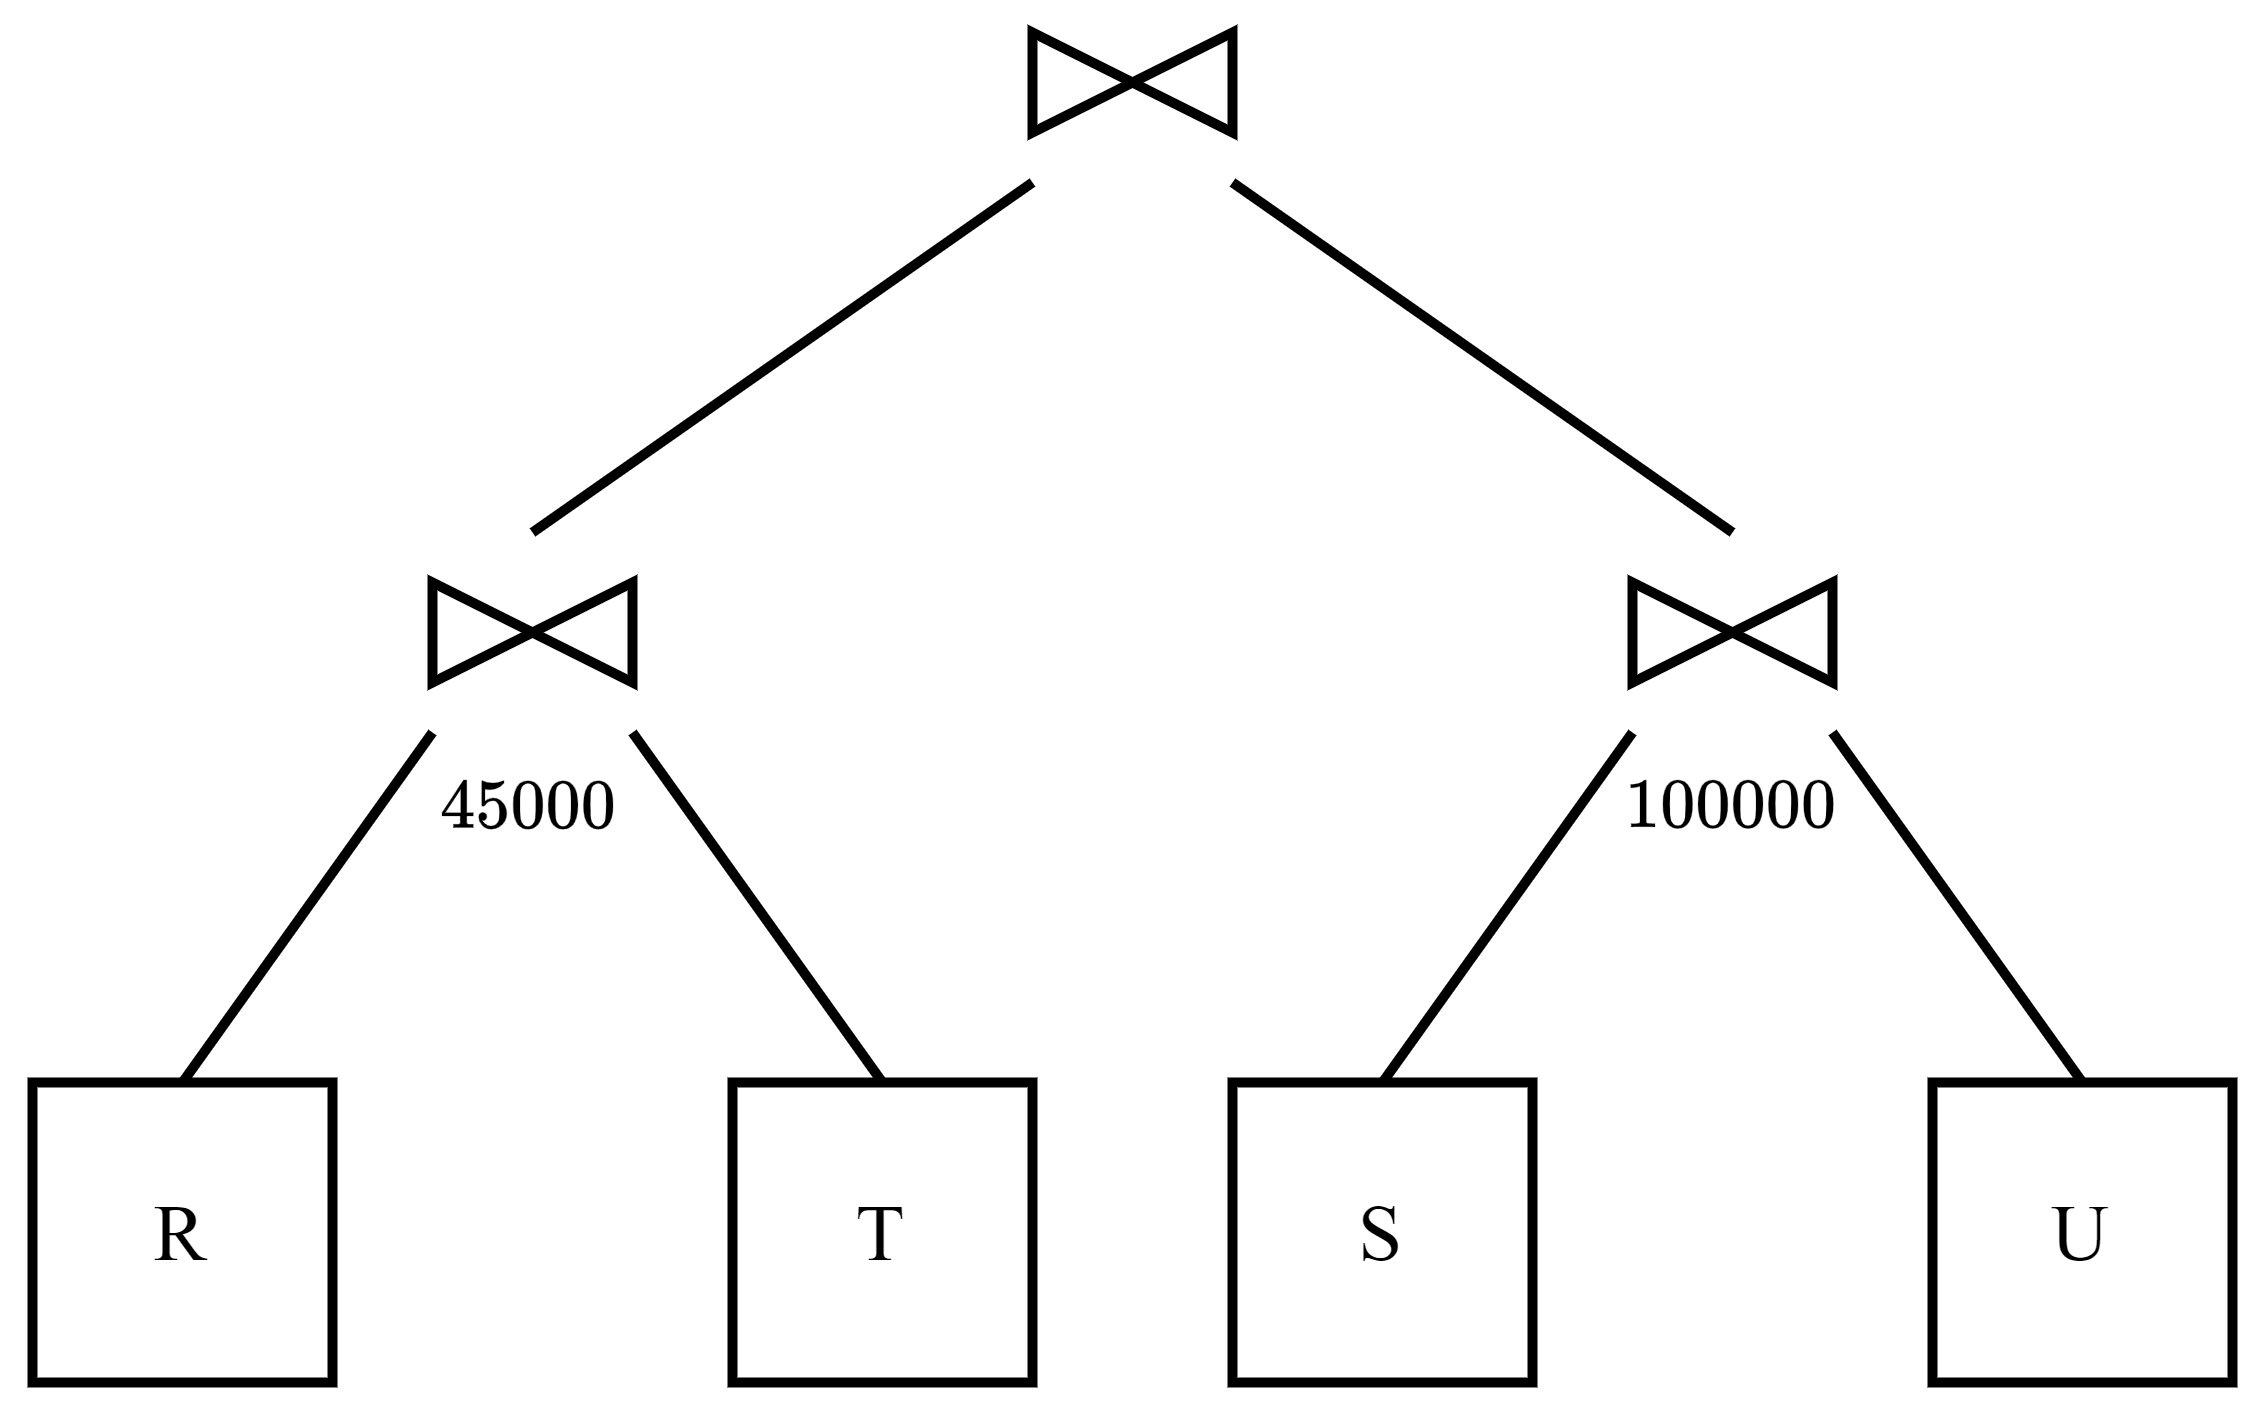
\includegraphics[width=0.5\textwidth]{img/E3-AB2.png}
            \end{figure}

            \newpage
            \item Para $(R \Join U) \Join (S \Join T)$
            \begin{figure}[H]
                \centering
                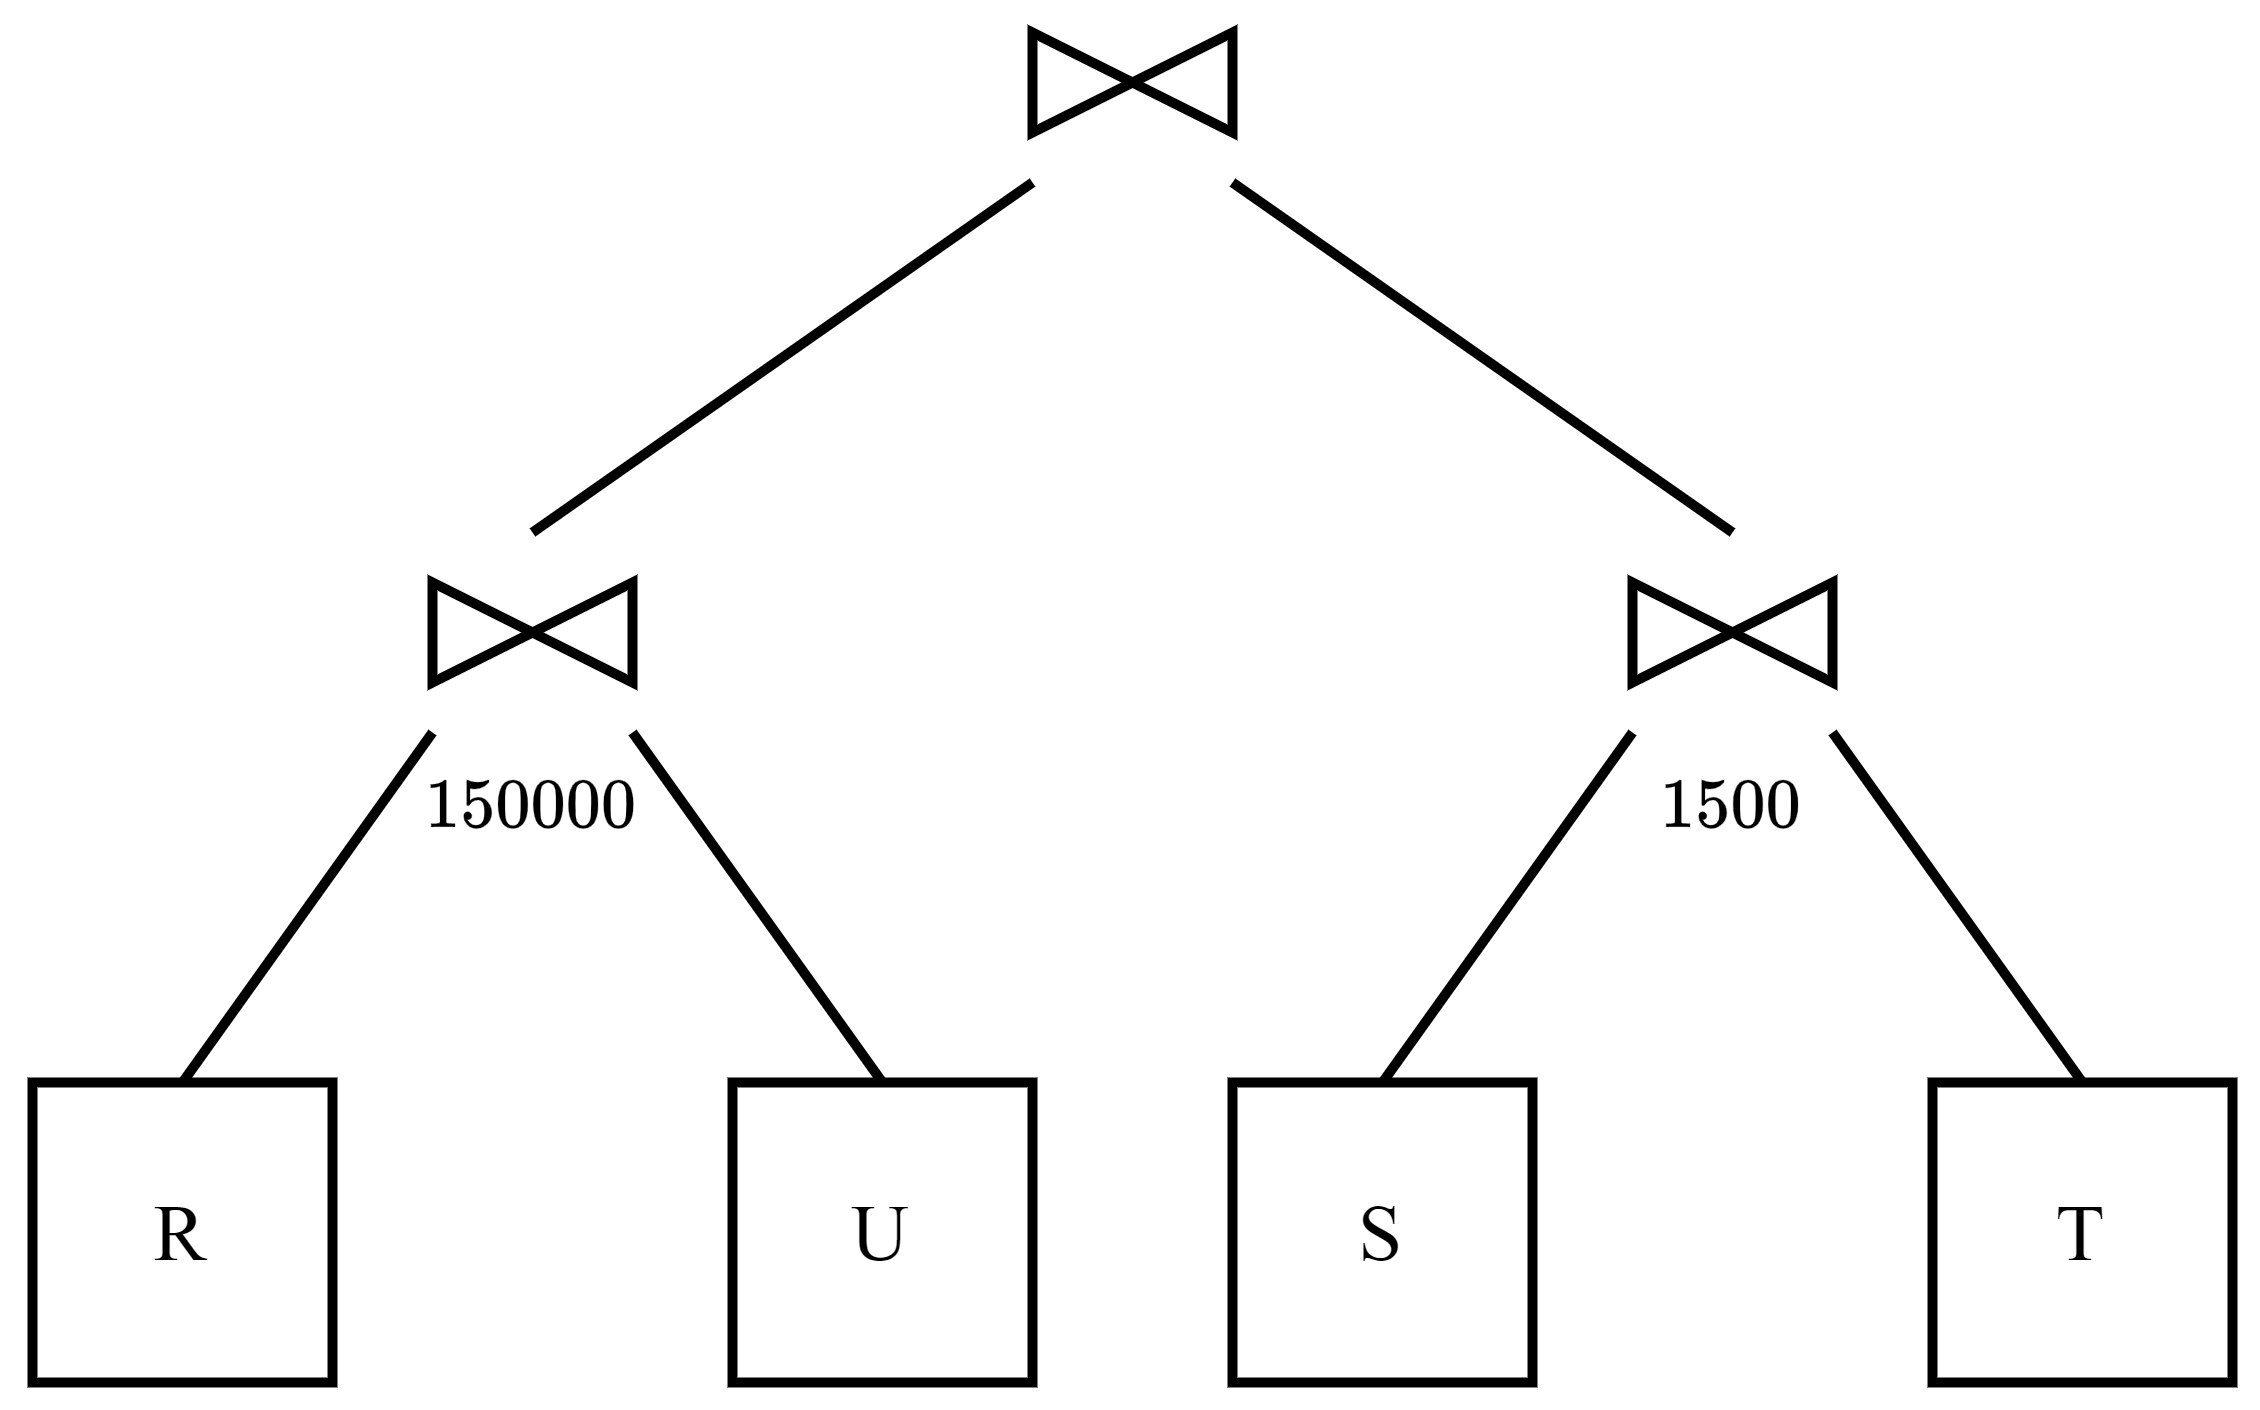
\includegraphics[width=0.5\textwidth]{img/E3-AB3.png}
            \end{figure}
        \end{itemize}
        
        \textbf{Agrupando tenemos que el costo es:}
        \begin{itemize}
            \item $(R \Join S) \Join (T \Join U) = 600 + 250 = 850$ *
            \item $(R \Join T) \Join (S \Join U) = 45000 + 100000 = 145000$
            \item $(R \Join U) \Join (S \Join T) = 150000 + 1500 = 151500$
        \end{itemize}

        \begin{equation*}
            \therefore \quad \text{El mejor plan es: } (R \Join S) \Join (T \Join U)
        \end{equation*}
    \end{enumerate}

    \newpage
    \item Suponer que tenemos las relaciones R(a, b), S(b, c), T(c, d) y U(d, e) con las siguientes características:
    \newparagraph
    \begin{minipage}{0.5\textwidth}
        \begin{itemize}
            \item T(R) = 50
            \item V(R, b) = 250
            \item T(S) = 55
            \item V(S, b) = 500
            \item V(S, c) = 5
        \end{itemize}
    \end{minipage}
    \hfill
    \begin{minipage}{0.5\textwidth}
        \begin{itemize}
            \item T(T) = 50
            \item V(T, c) = 15
            \item V(T, d) = 500
            \item T(U) = 45
            \item V(U, d) = 50
        \end{itemize}
    \end{minipage}
    \begin{center}
        \begin{tabular}{|c|c|c|c|}
            \hline
            R & S & T & U \\
            \hline
            T(R) = 50 & T(S) = 55 & T(T) = 50 & T(U) = 45 \\
            V(R, b) = 250 & V(S, b) = 500 & & \\
            & V(S, c) = 5 & V(T, c) = 15 & \\
            & & V(T, d) = 500 & V(U, d) = 50 \\
            \hline
        \end{tabular}
    \end{center}
    \newparagraph

    \textbf{Paso a paso:}
    \begin{enumerate}[label=\arabic*)]
        \item Costos simples.
        \begin{center}
            \begin{tabular}{|r|c|c|c|c|}
                \hline
                & R & S & T & U \\
                \hline
                \textbf{Tamaño} & 50 & 55 & 50 & 45 \\
                \hline
                \textbf{Costo}  & 0 & 0 & 0 & 0 \\
                \hline
                \textbf{Mejor Plan} & R & S & T & U \\
                \hline
            \end{tabular}
        \end{center}
        \newparagraph

        \item Calculo simples.
        \newparagraph
        \begin{minipage}{0.5\textwidth}
            \begin{itemize}
                \item $T(R) = 50$
                \item $T(S) = 55$
            \end{itemize}
        \end{minipage}
        \hfill
        \begin{minipage}{0.5\textwidth}
            \begin{itemize}
                \item $T(T) = 50$
                \item $T(U) = 45$ *
            \end{itemize}
        \end{minipage}
        \newparagraph

        \item Costo pares.
        \begin{center}
            \begin{tabular}{|r|c|c|c|c|c|c|c|}
                \hline
                & $\{R, \; S\}$ & $\{R, \; T\}$ & $\{R, \; U\}$ & $\{S, \; T\}$ & $\{S, \; U\}$ & $\{T, \; U\}$ \\
                \hline
                \textbf{Tamaño} & 5.5 & 2500 & 2250 & 183.34 & 2475 & 4.5 \\
                \hline
                \textbf{Costo}  & 0 & 0 & 0 & 0 & 0 & 0 \\
                \hline
                \textbf{Mejor Plan} & $R \Join S$ & $R \Join T$ & $R \Join U$ & $S \Join T$ & $S \Join U$ & $T \Join U$ \\
                \hline
            \end{tabular}
        \end{center}
        \newparagraph

        \item Calculo pares.
        \begin{itemize}
            \item $T(R \Join S) =  \displaystyle\frac{T(R) \cdot T(S)}{\text{max}\{V(R,b), \; V(S,b)\}} = \frac{50 \cdot 55}{\text{max} \{250, 500\}} = \frac{2750}{500} = \colorbox{gray!20}{5.5}$ \newparagraph
            
            \newpage
            \item $T(R \Join T) =  \displaystyle\frac{T(R) \cdot T(T)}{\text{max}\{V(R,-), \; V(T,-)\}} = 50 \cdot 50 = \colorbox{gray!20}{2500}$ \newparagraph
            
            \item $T(R \Join U) =  \displaystyle\frac{T(R) \cdot T(U)}{\text{max}\{V(R,-), \; V(U,-)\}} = 50 \cdot 45 = \colorbox{gray!20}{2250}$ \newparagraph
            
            \item $T(S \Join T) =  \displaystyle\frac{T(S) \cdot T(T)}{\text{max}\{V(S,c), \; V(T,c)\}} = \frac{55 \cdot 50}{\text{max} \{5, 15\}} = \frac{2750}{15} = \colorbox{gray!20}{183.34}$ \newparagraph
            
            \item $T(S \Join U) =  \displaystyle\frac{T(S) \cdot T(U)}{\text{max}\{V(S,-), \; V(U,-)\}} = 55 \cdot 45 = \colorbox{gray!20}{2475}$ \newparagraph
            
            \item $T(T \Join U) =  \displaystyle\frac{T(T) \cdot T(U)}{\text{max}\{V(T,d), \; V(U,d)\}} = \frac{50 \cdot 45}{\text{max} \{500, 50\}} = \frac{2250}{500} = \colorbox{gray!20}{4.5}$ \newparagraph
        \end{itemize}

        \item Costo tripletas.
        \begin{center}
            \begin{tabular}{|r|c|c|c|c|}
                \hline
                & $\{R, \; S, \; T\}$ & $\{R, \; S, \; U\}$ & $\{R, \; T, \; U\}$ & $\{S, \; T, \; U\}$ \\
                \hline
                \textbf{Tamaño} & 18.34 & 247.5 & 225 & 16.5 \\
                \hline
                \textbf{Costo}  & 5.5 & 5.5 & 4.5 & 4.5 \\
                \hline
                \textbf{Mejor Plan} & $(R \Join S) \Join T$ & $(R \Join S) \Join U$ & $(T \Join U) \Join R$ & $(T \Join U) \Join S$ \\
                \hline
            \end{tabular}
        \end{center}
        \newparagraph

        \item Calculo tripletas.
        \begin{itemize}
            \item Para $\{R, \; S, \; T\}$
            \begin{itemize}
                \item $T(R \Join S) = \colorbox{gray!20}{5.5}$ *
                \item $T(R \Join T) = 2500$
                \item $T(S \Join T) = 193.34$
            \end{itemize}
            \begin{align*}
                T((R \Join S) \Join T) &= \displaystyle\frac{T(R \Join S) \cdot T(T)}{\text{max}\{V((R \Join S), c), \; V(T,c)\}} \\
                &= \frac{5.5 \cdot 50}{\text{max}\{5, 15\}} = \frac{275}{15} = \colorbox{gray!20}{18.34}
            \end{align*}
            \newparagraph

            \newpage
            \item Para $\{R, \; S, \; U\}$
            \begin{itemize}
                \item $T(R \Join S) = \colorbox{gray!20}{5.5}$ *
                \item $T(R \Join U) = 2250$
                \item $T(S \Join U) = 2475$
            \end{itemize}
            \begin{align*}
                T((R \Join S) \Join U) &= \displaystyle\frac{T(R \Join S) \cdot T(U)}{\text{max}\{V(R\Join S,-), \; V(U,-)\}} \\
                &= 5.5 \cdot 45 = \colorbox{gray!20}{247.5}
            \end{align*}
            \newparagraph

            \item Para $\{R, \; T, \; U\}$
            \begin{itemize}
                \item $T(R \Join T) = 2500$
                \item $T(R \Join U) = 2250$
                \item $T(T \Join U) = \colorbox{gray!20}{4.5}$ *
            \end{itemize}
            \begin{align*}
                T((T \Join U) \Join R) &= \displaystyle\frac{T(T \Join U) \cdot T(R)}{\text{max}\{V(T \Join U,-), \; V(R,-)\}} \\
                &= 4.5 \cdot 50 = \colorbox{gray!20}{225}
            \end{align*}
            \newparagraph

            \item Para $\{S, \; T, \; U\}$
            \begin{itemize}
                \item $T(S \Join T) = 183.34$
                \item $T(S \Join U) = 2475$
                \item $T(T \Join U) = \colorbox{gray!20}{4.5}$ *
            \end{itemize}
            \begin{align*}
                T((T \Join U) \Join S) &= \displaystyle\frac{T(T \Join U) \cdot T(S)}{\text{max}\{V((T \Join U),c), \; V(S,c)\}} \\
                &= \frac{4.5 \cdot 55}{\text{max}\{5, 15\}} = \frac{247.5}{15} = \colorbox{gray!20}{16.5}
            \end{align*}
            \newparagraph
        \end{itemize}
        
        \item Arboles.
        \begin{itemize}
            \item Para $\{R, \; S, \; T\}$
            \begin{figure}[H]
                \centering
                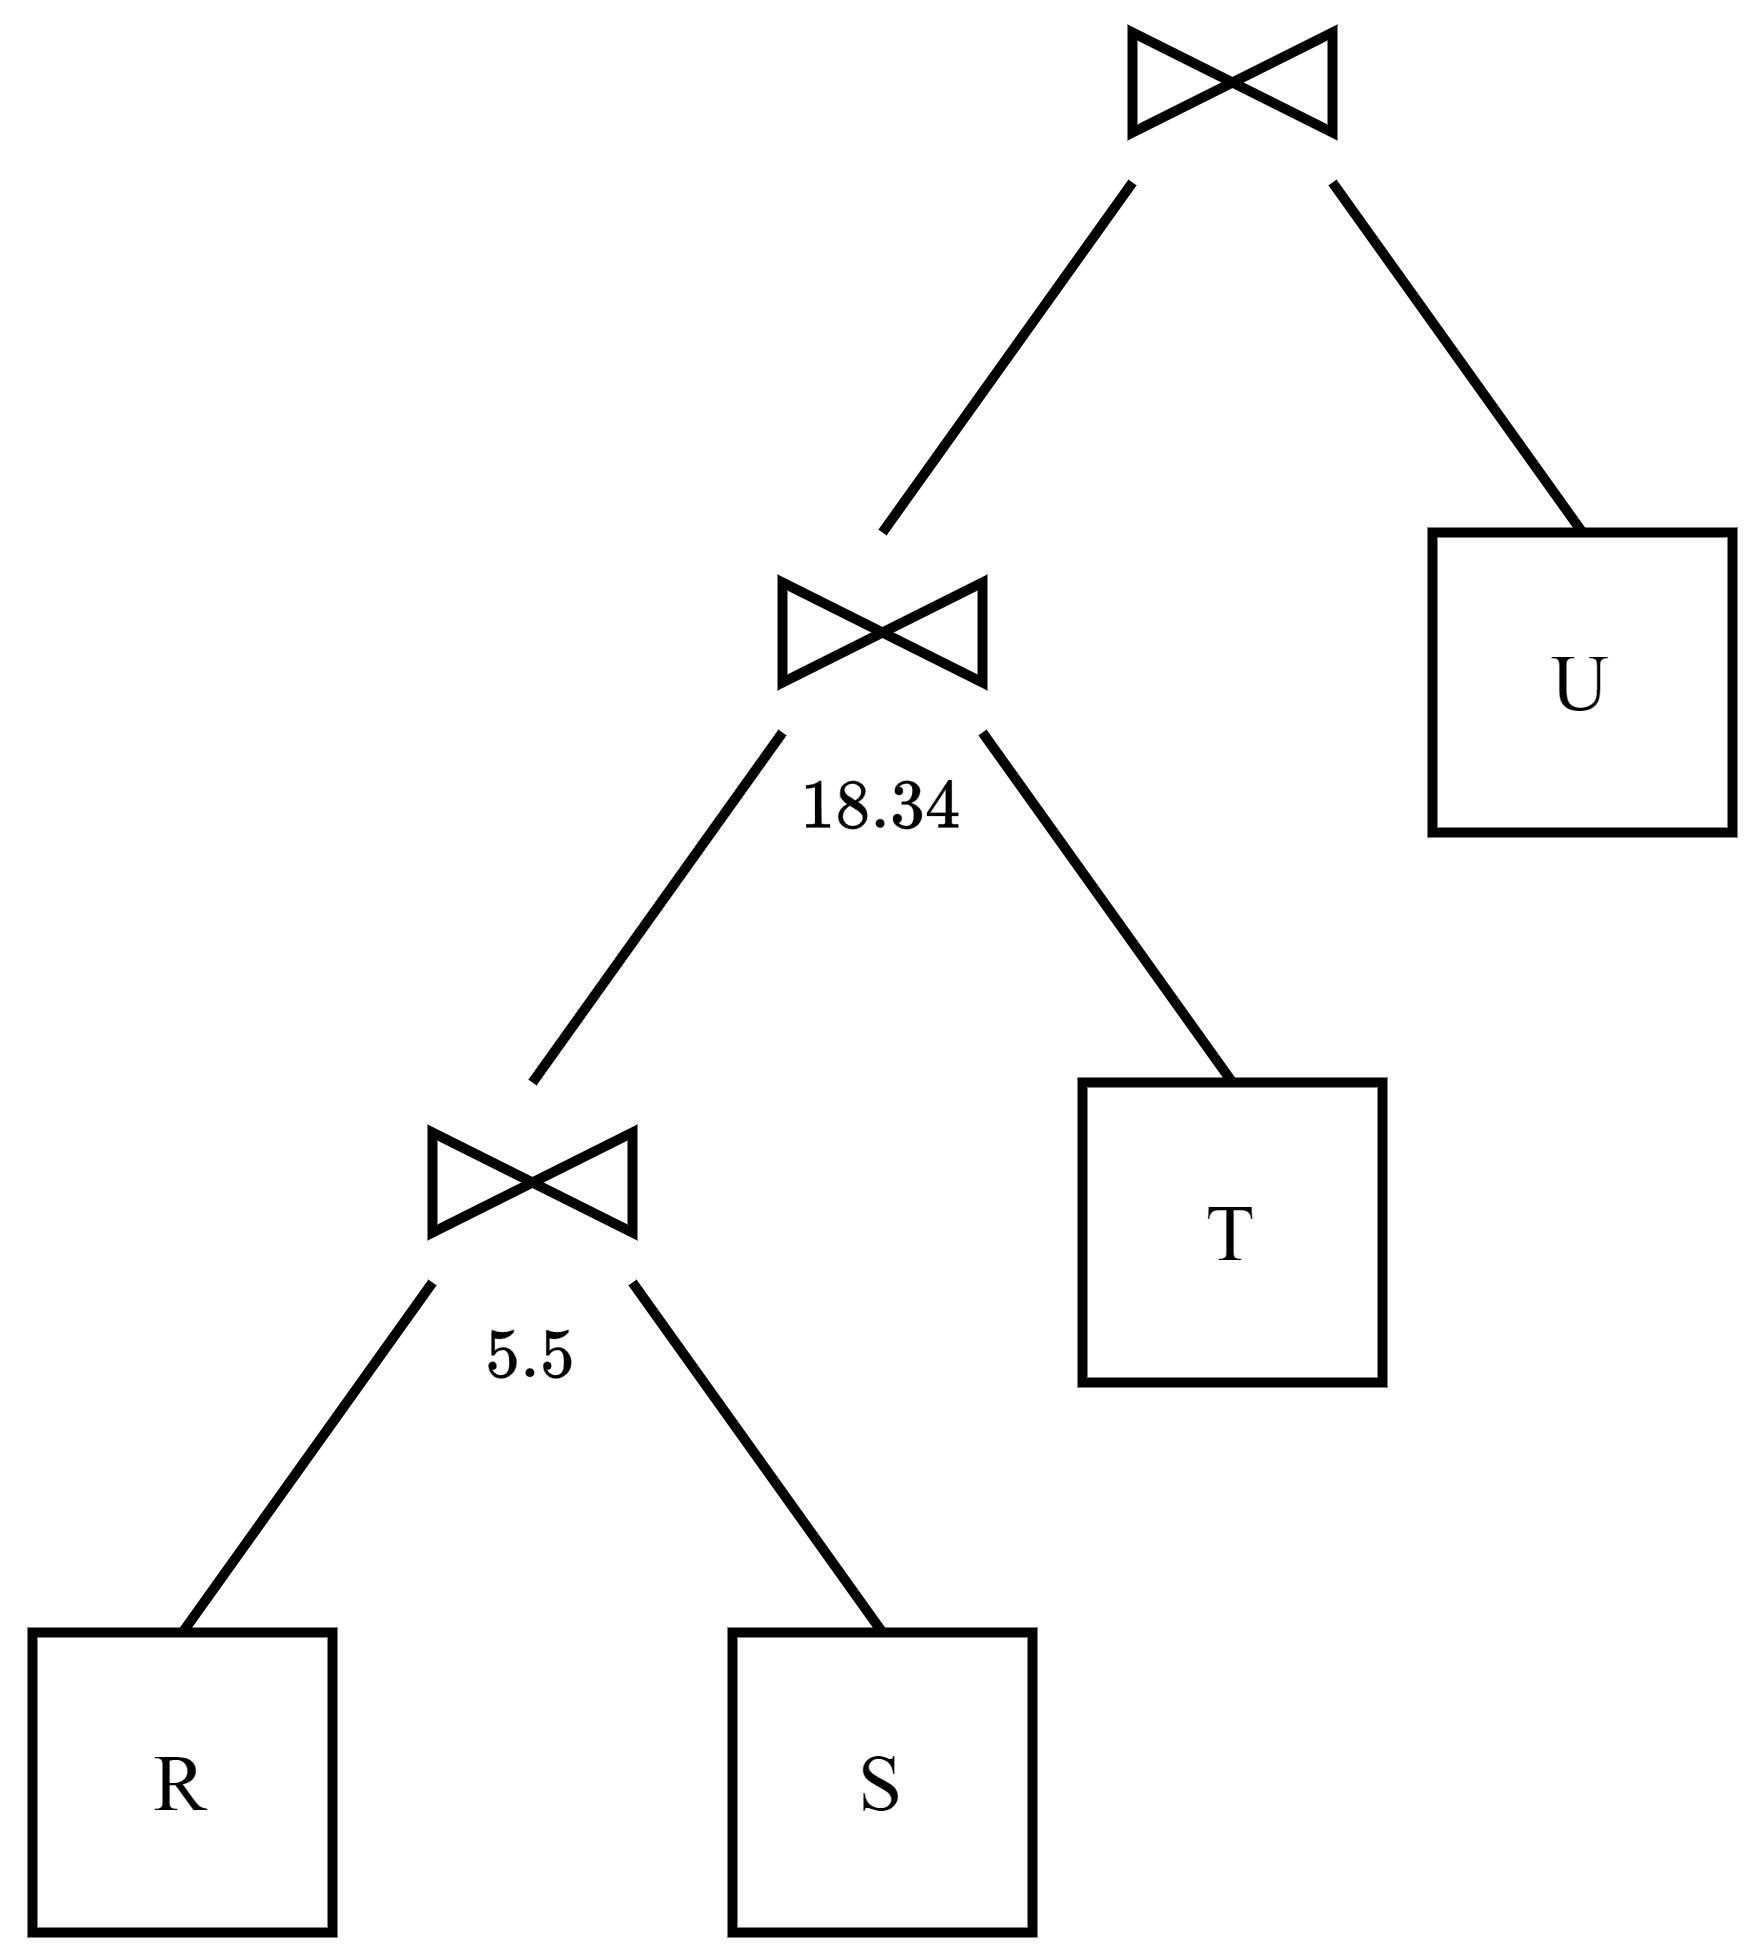
\includegraphics[width=0.35\textwidth]{img/E4-A1.png}
            \end{figure}

            \newpage
            \item Para $\{R, \; S, \; U\}$
            \begin{figure}[H]
                \centering
                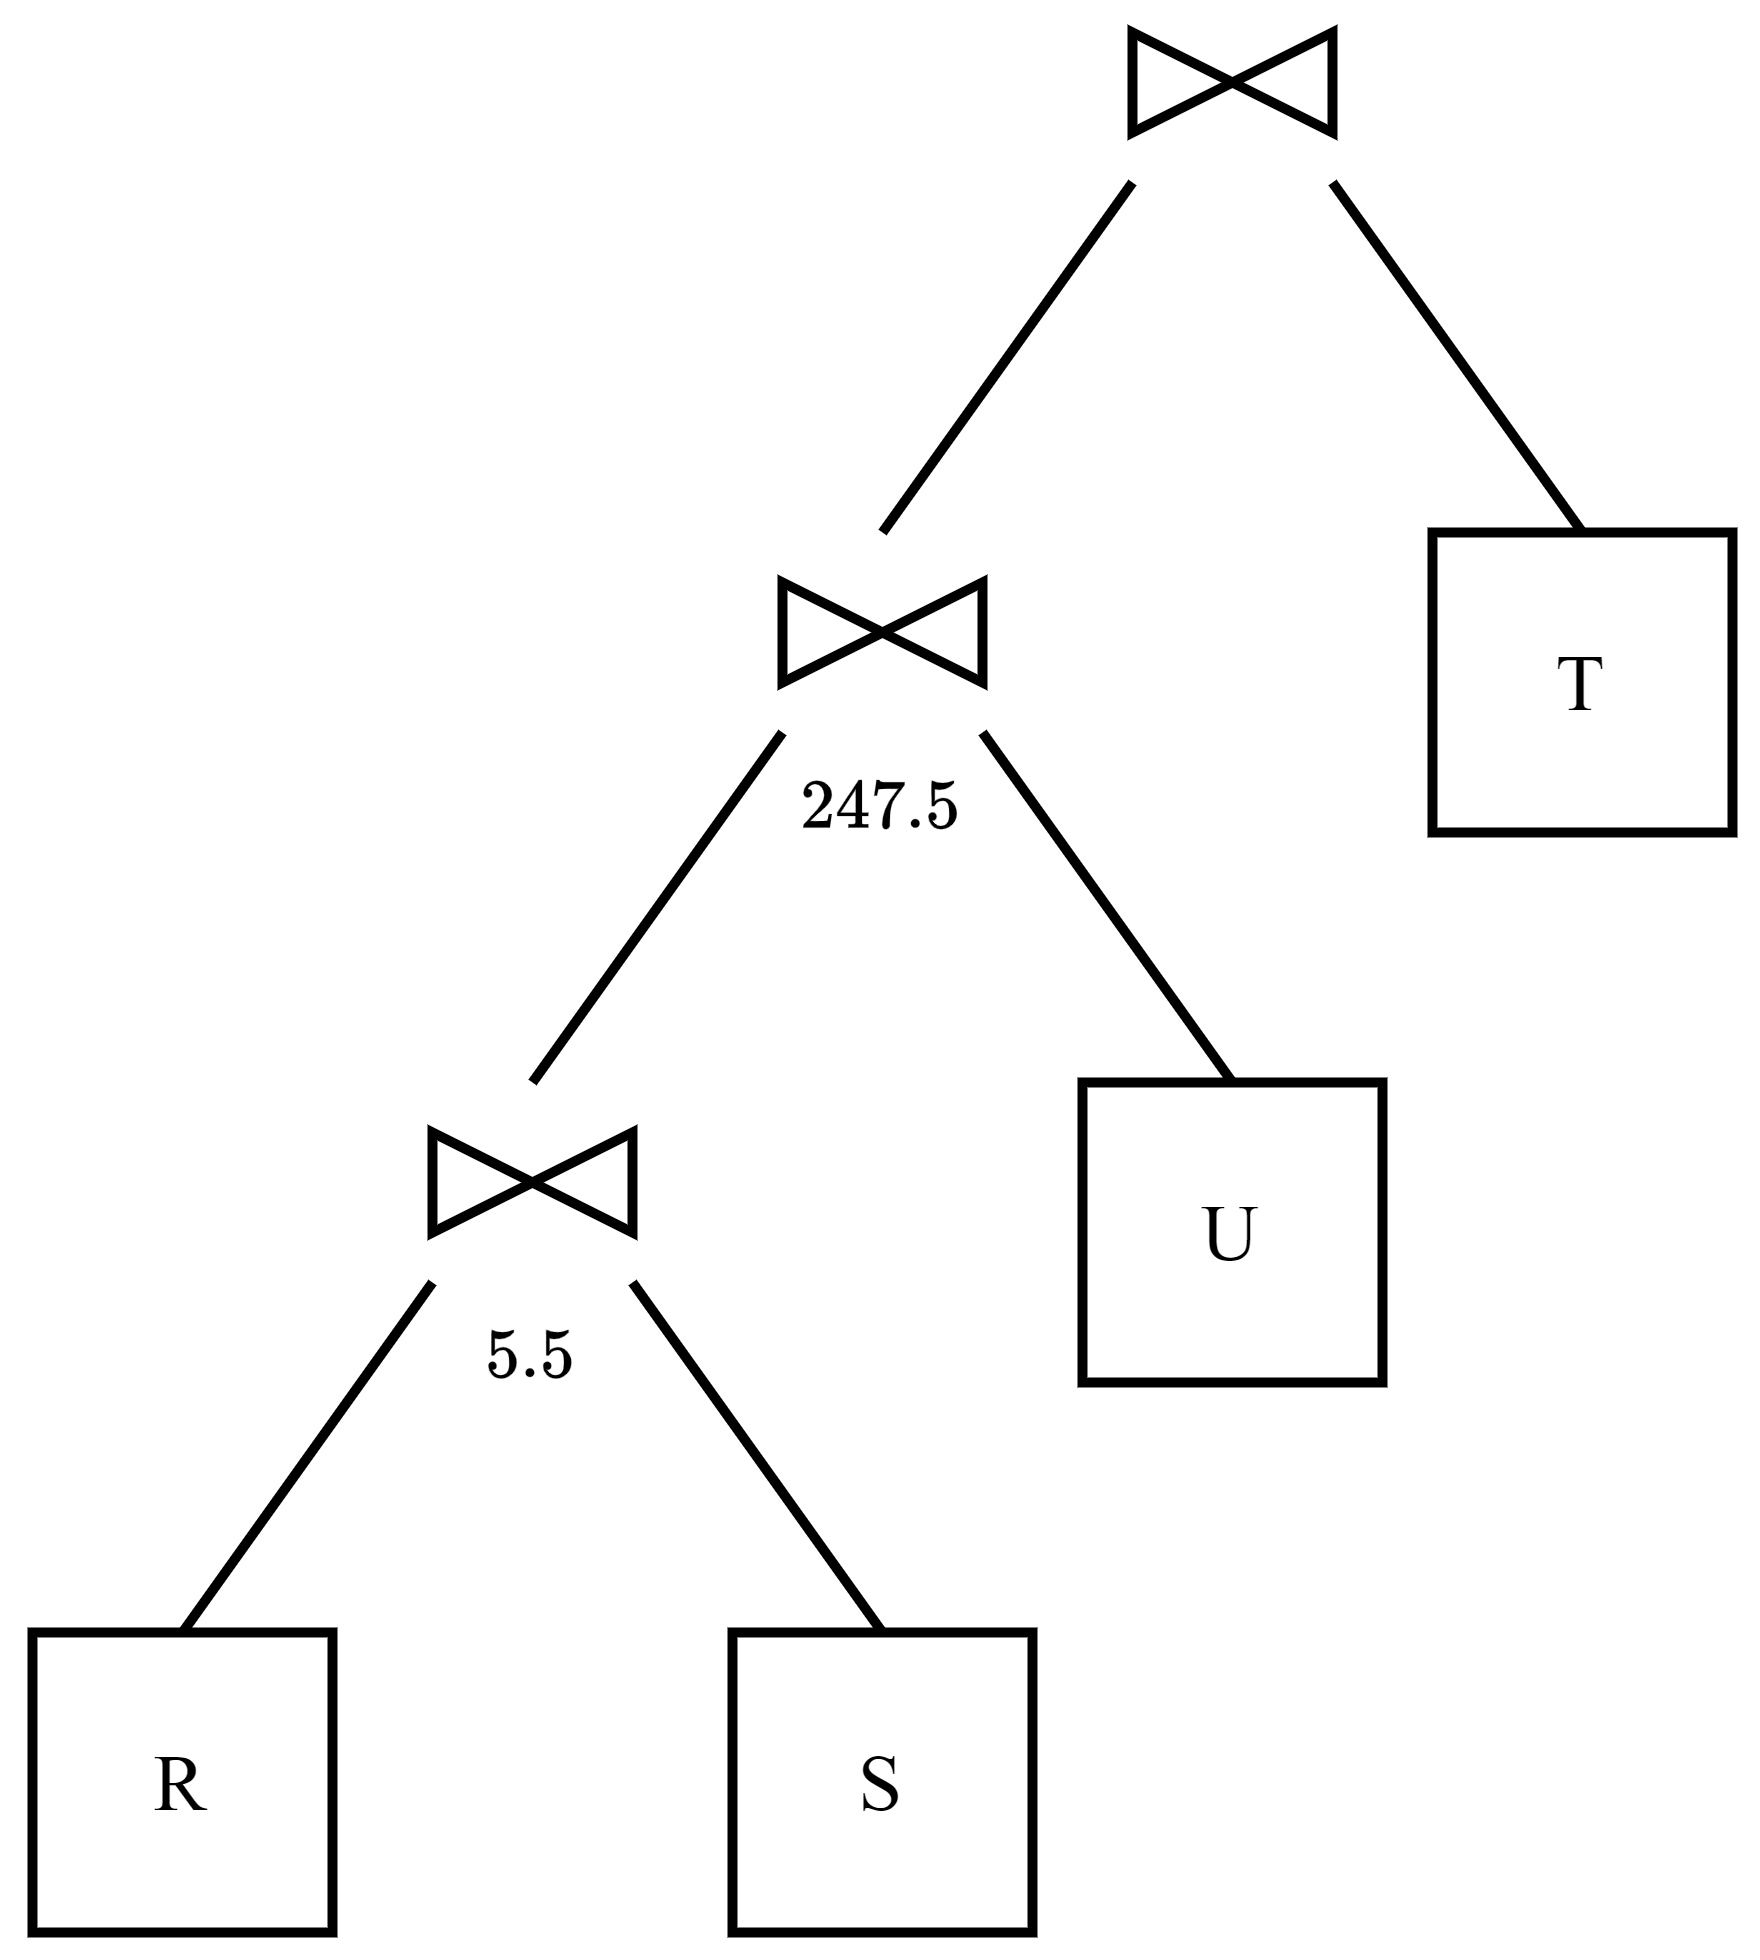
\includegraphics[width=0.35\textwidth]{img/E4-A2.png}
            \end{figure}

            \item Para $\{R, \; T, \; U\}$
            \begin{figure}[H]
                \centering
                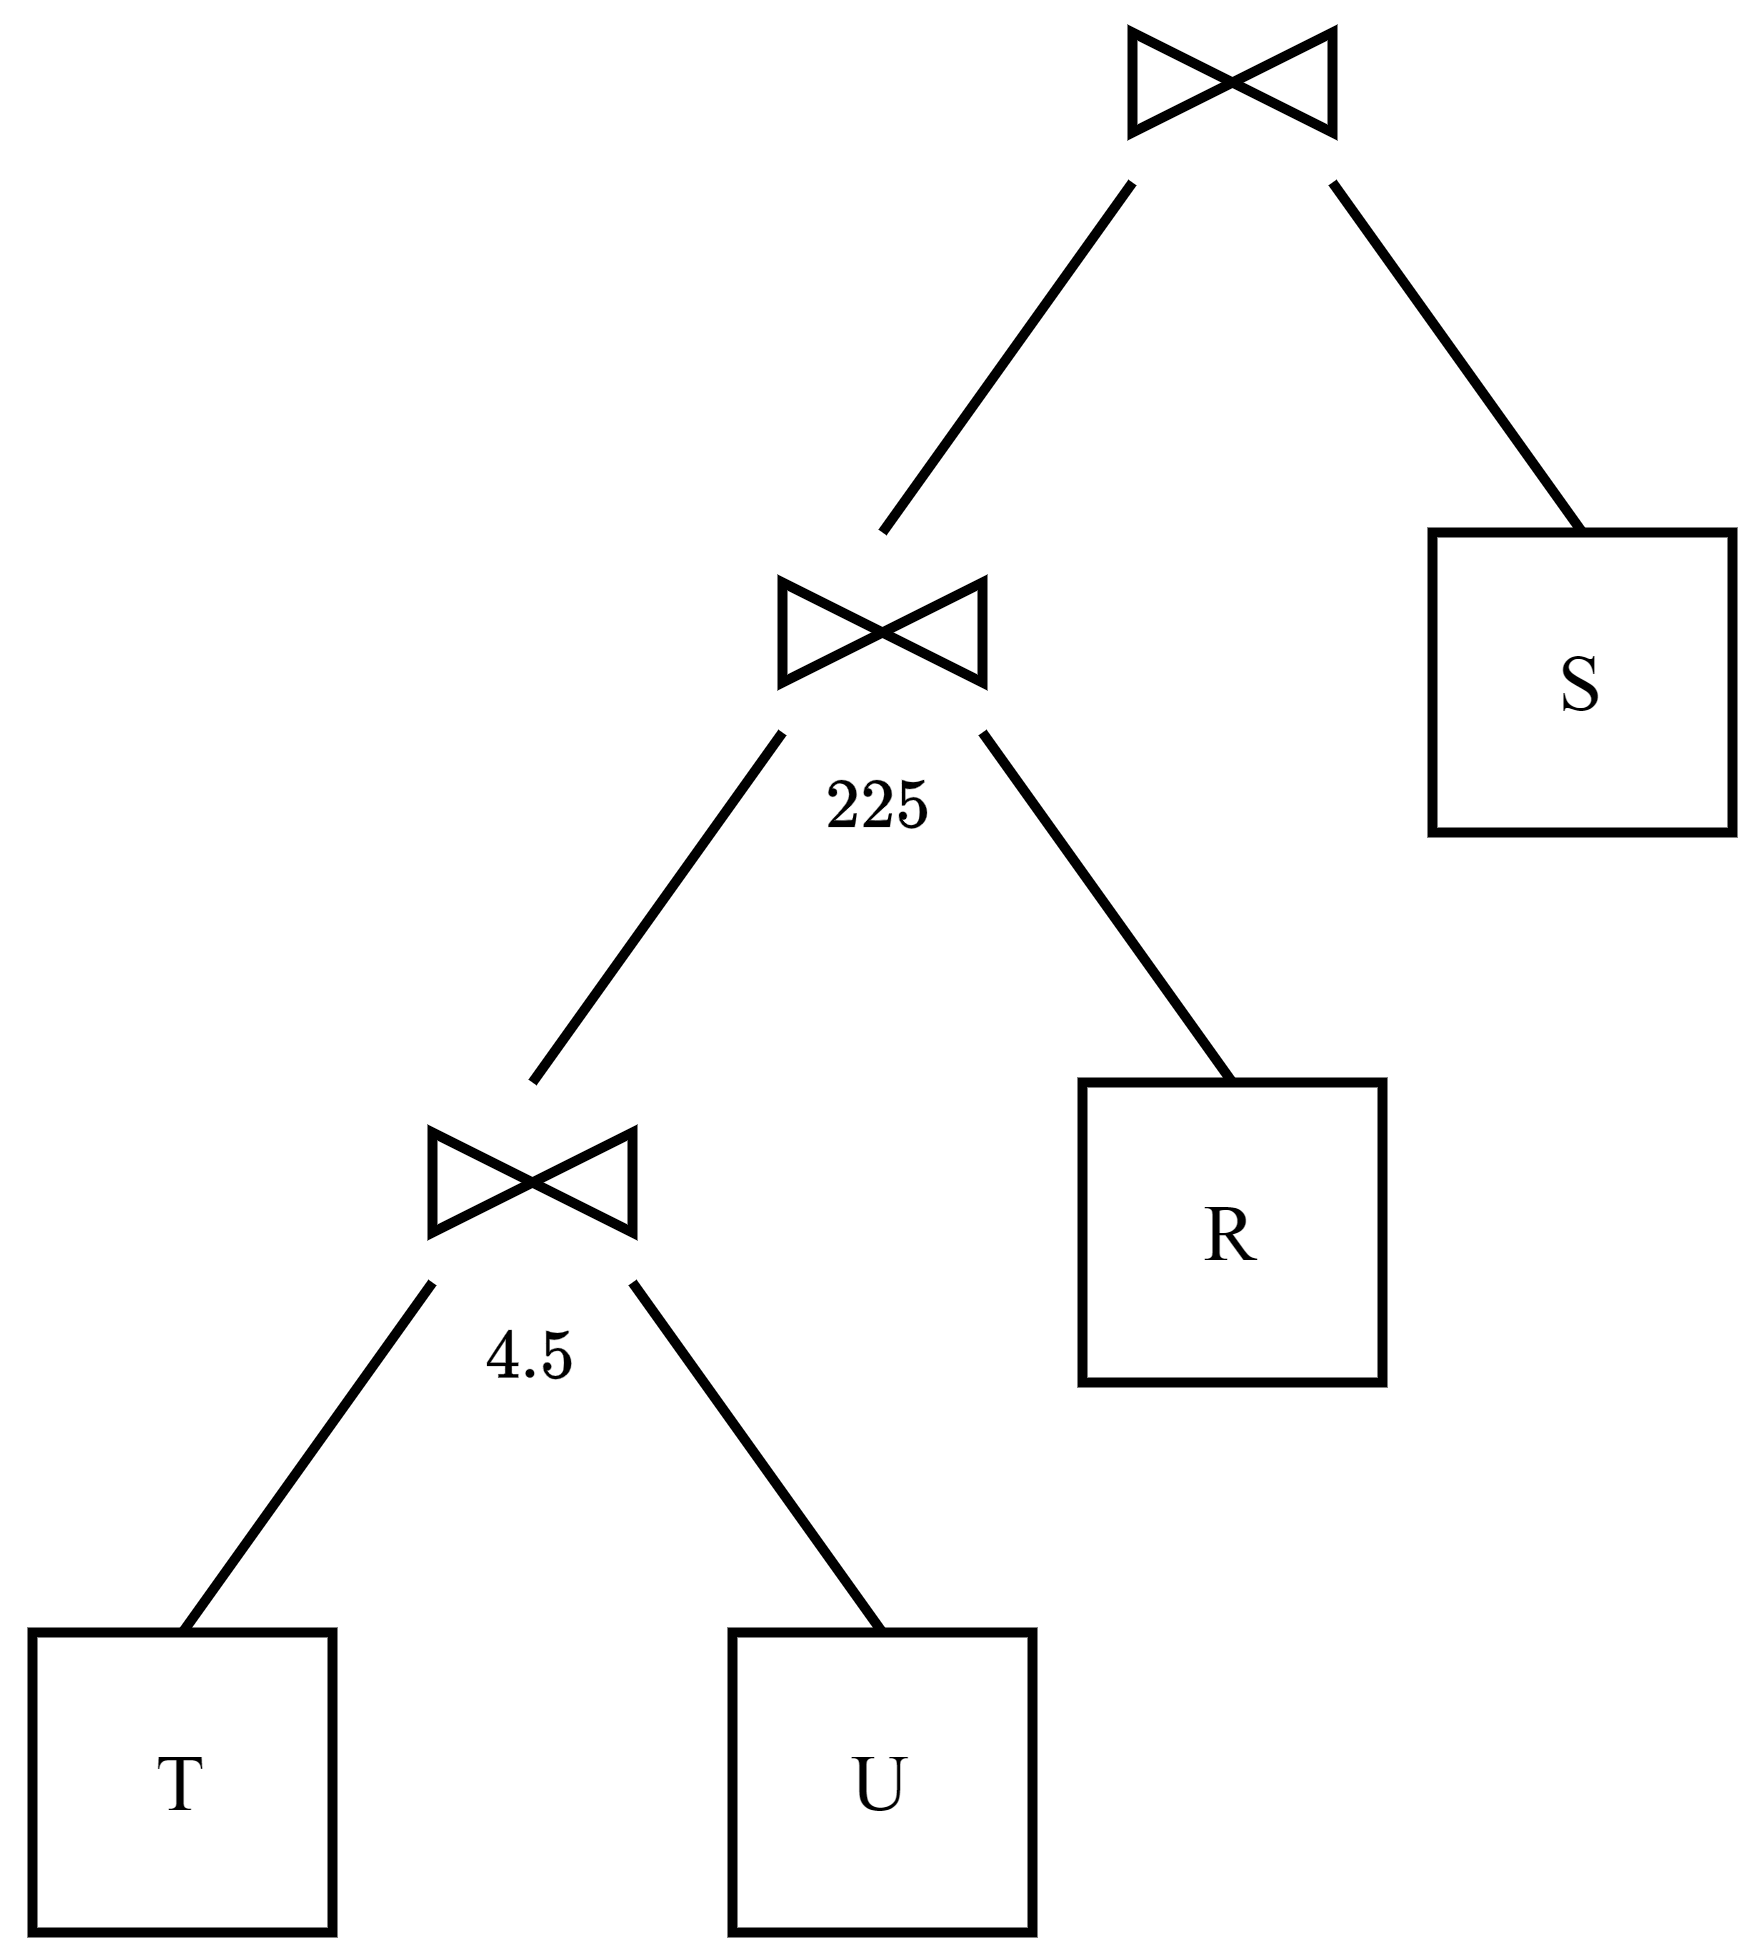
\includegraphics[width=0.35\textwidth]{img/E4-A3.png}
            \end{figure}

            \item Para $\{S, \; T, \; U\}$
            \begin{figure}[H]
                \centering
                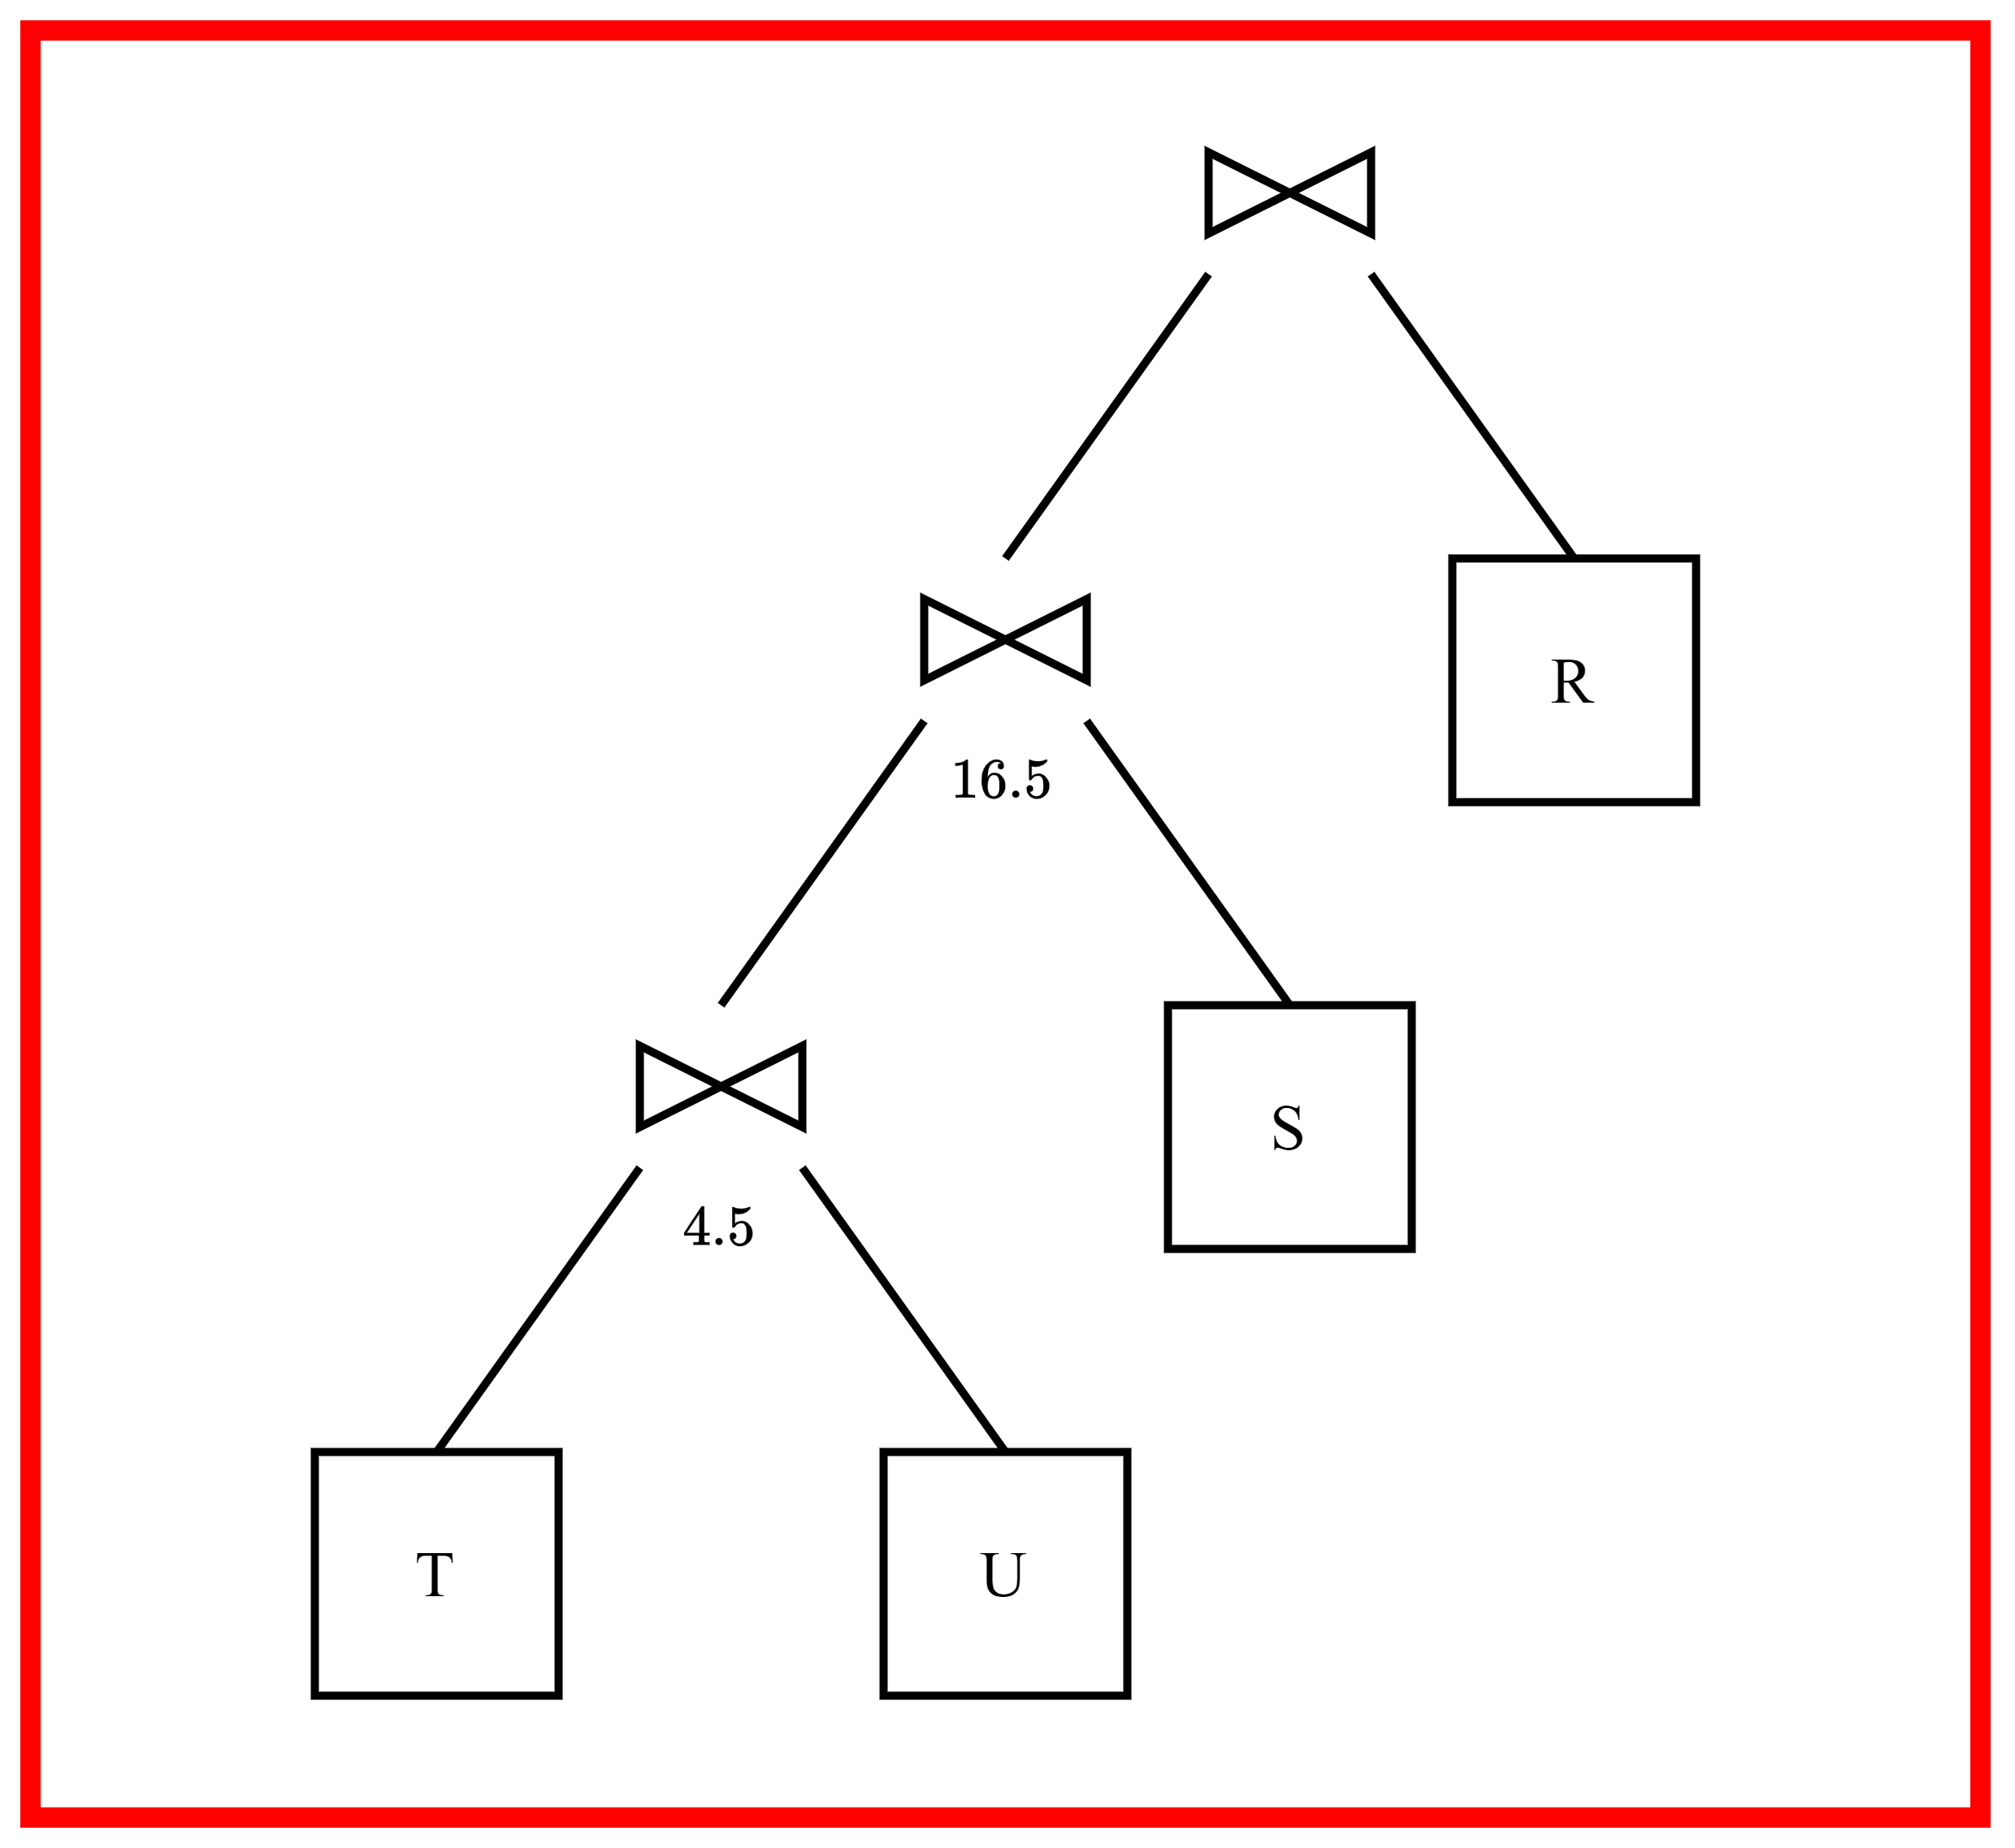
\includegraphics[width=0.5\textwidth]{img/E4-A4.png}
            \end{figure}
        \end{itemize}

        \newpage
        \textbf{Agrupando tenemos que el costo es:}
        \begin{itemize}
            \item $(((R \Join S) \Join T) \Join U) = 5.5 + 18.34 = 23.84$
            \item $(((R \Join S) \Join U) \Join T) = 5.5 + 247.5 = 253$
            \item $(((T \Join U) \Join R) \Join S) = 4.5 + 225 = 229.5$
            \item $(((T \Join U) \Join S) \Join R) = 16.5 + 4.5 = 21$ *
        \end{itemize}

        \begin{equation*}
            \therefore \quad \text{El mejor plan es: } (((T \Join U) \Join S) \Join R)
        \end{equation*}
        \newparagraph

        \item Realizando el árbol balanceado.
        \begin{itemize}
            \item Para $(R \Join S) \Join (T \Join U)$
            \begin{figure}[H]
                \centering
                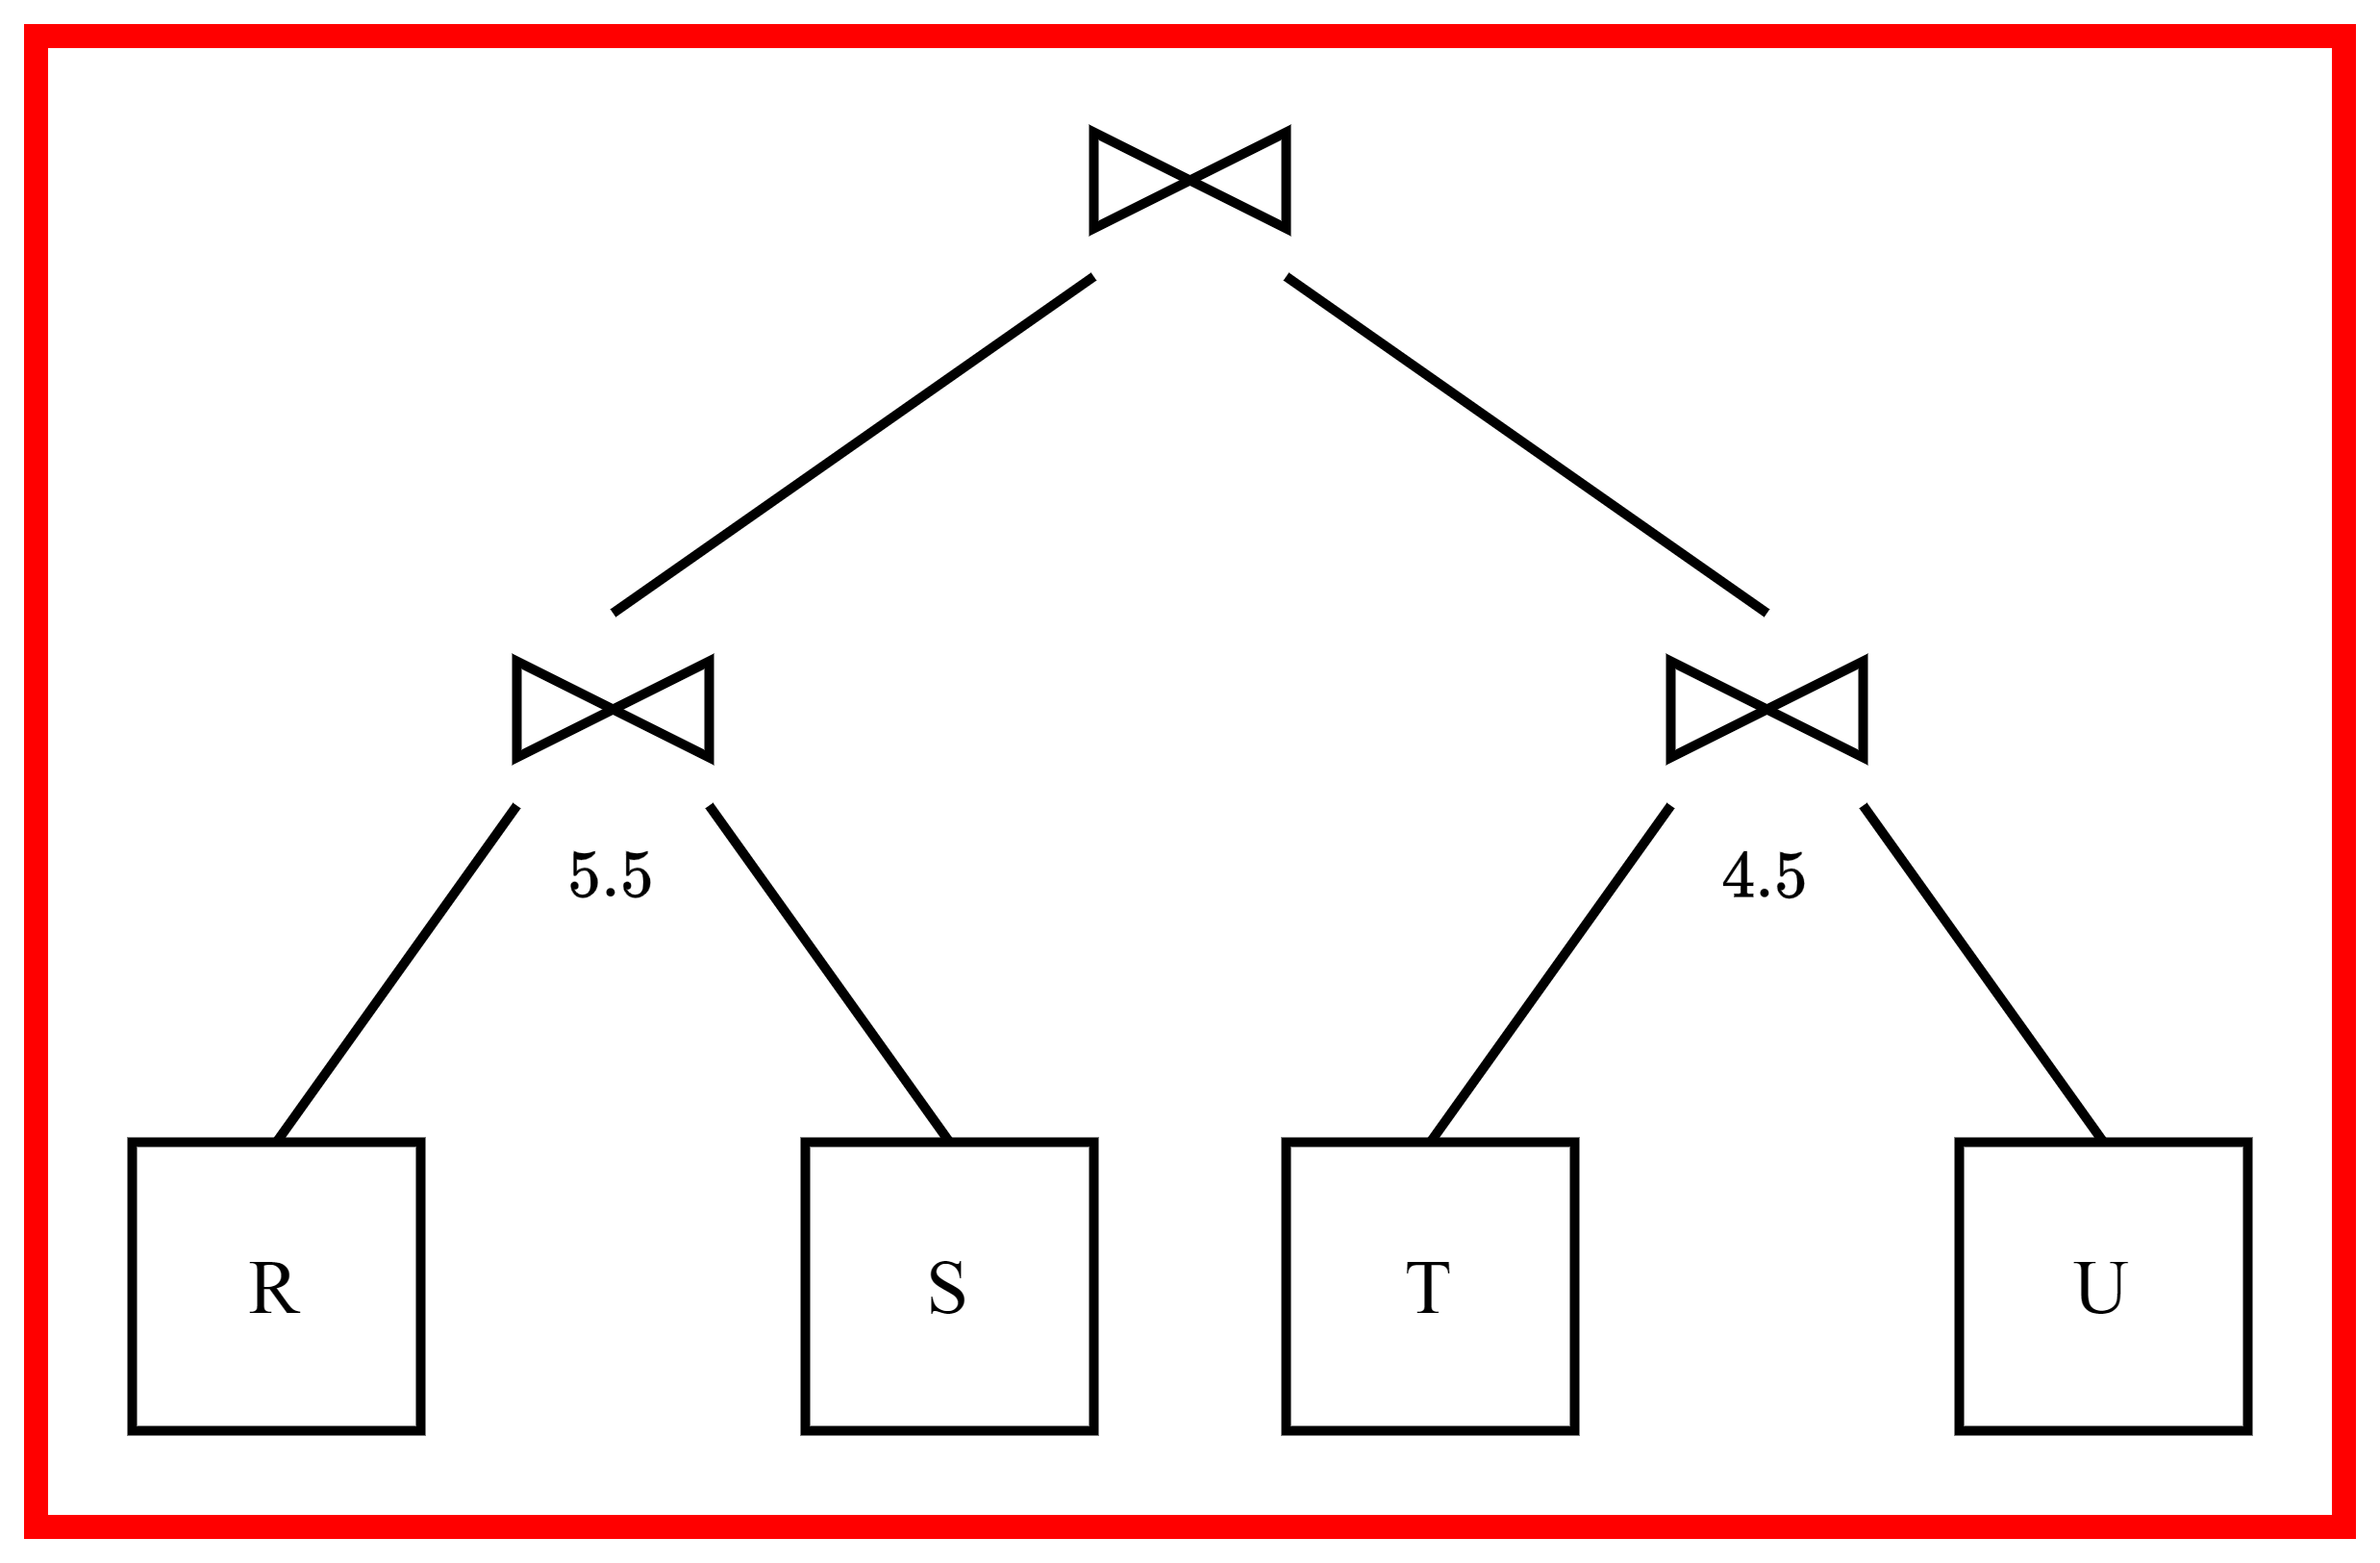
\includegraphics[width=0.55\textwidth]{img/E4-AB1.png}
            \end{figure}

            \item Para $(R \Join T) \Join (S \Join U)$
            \begin{figure}[H]
                \centering
                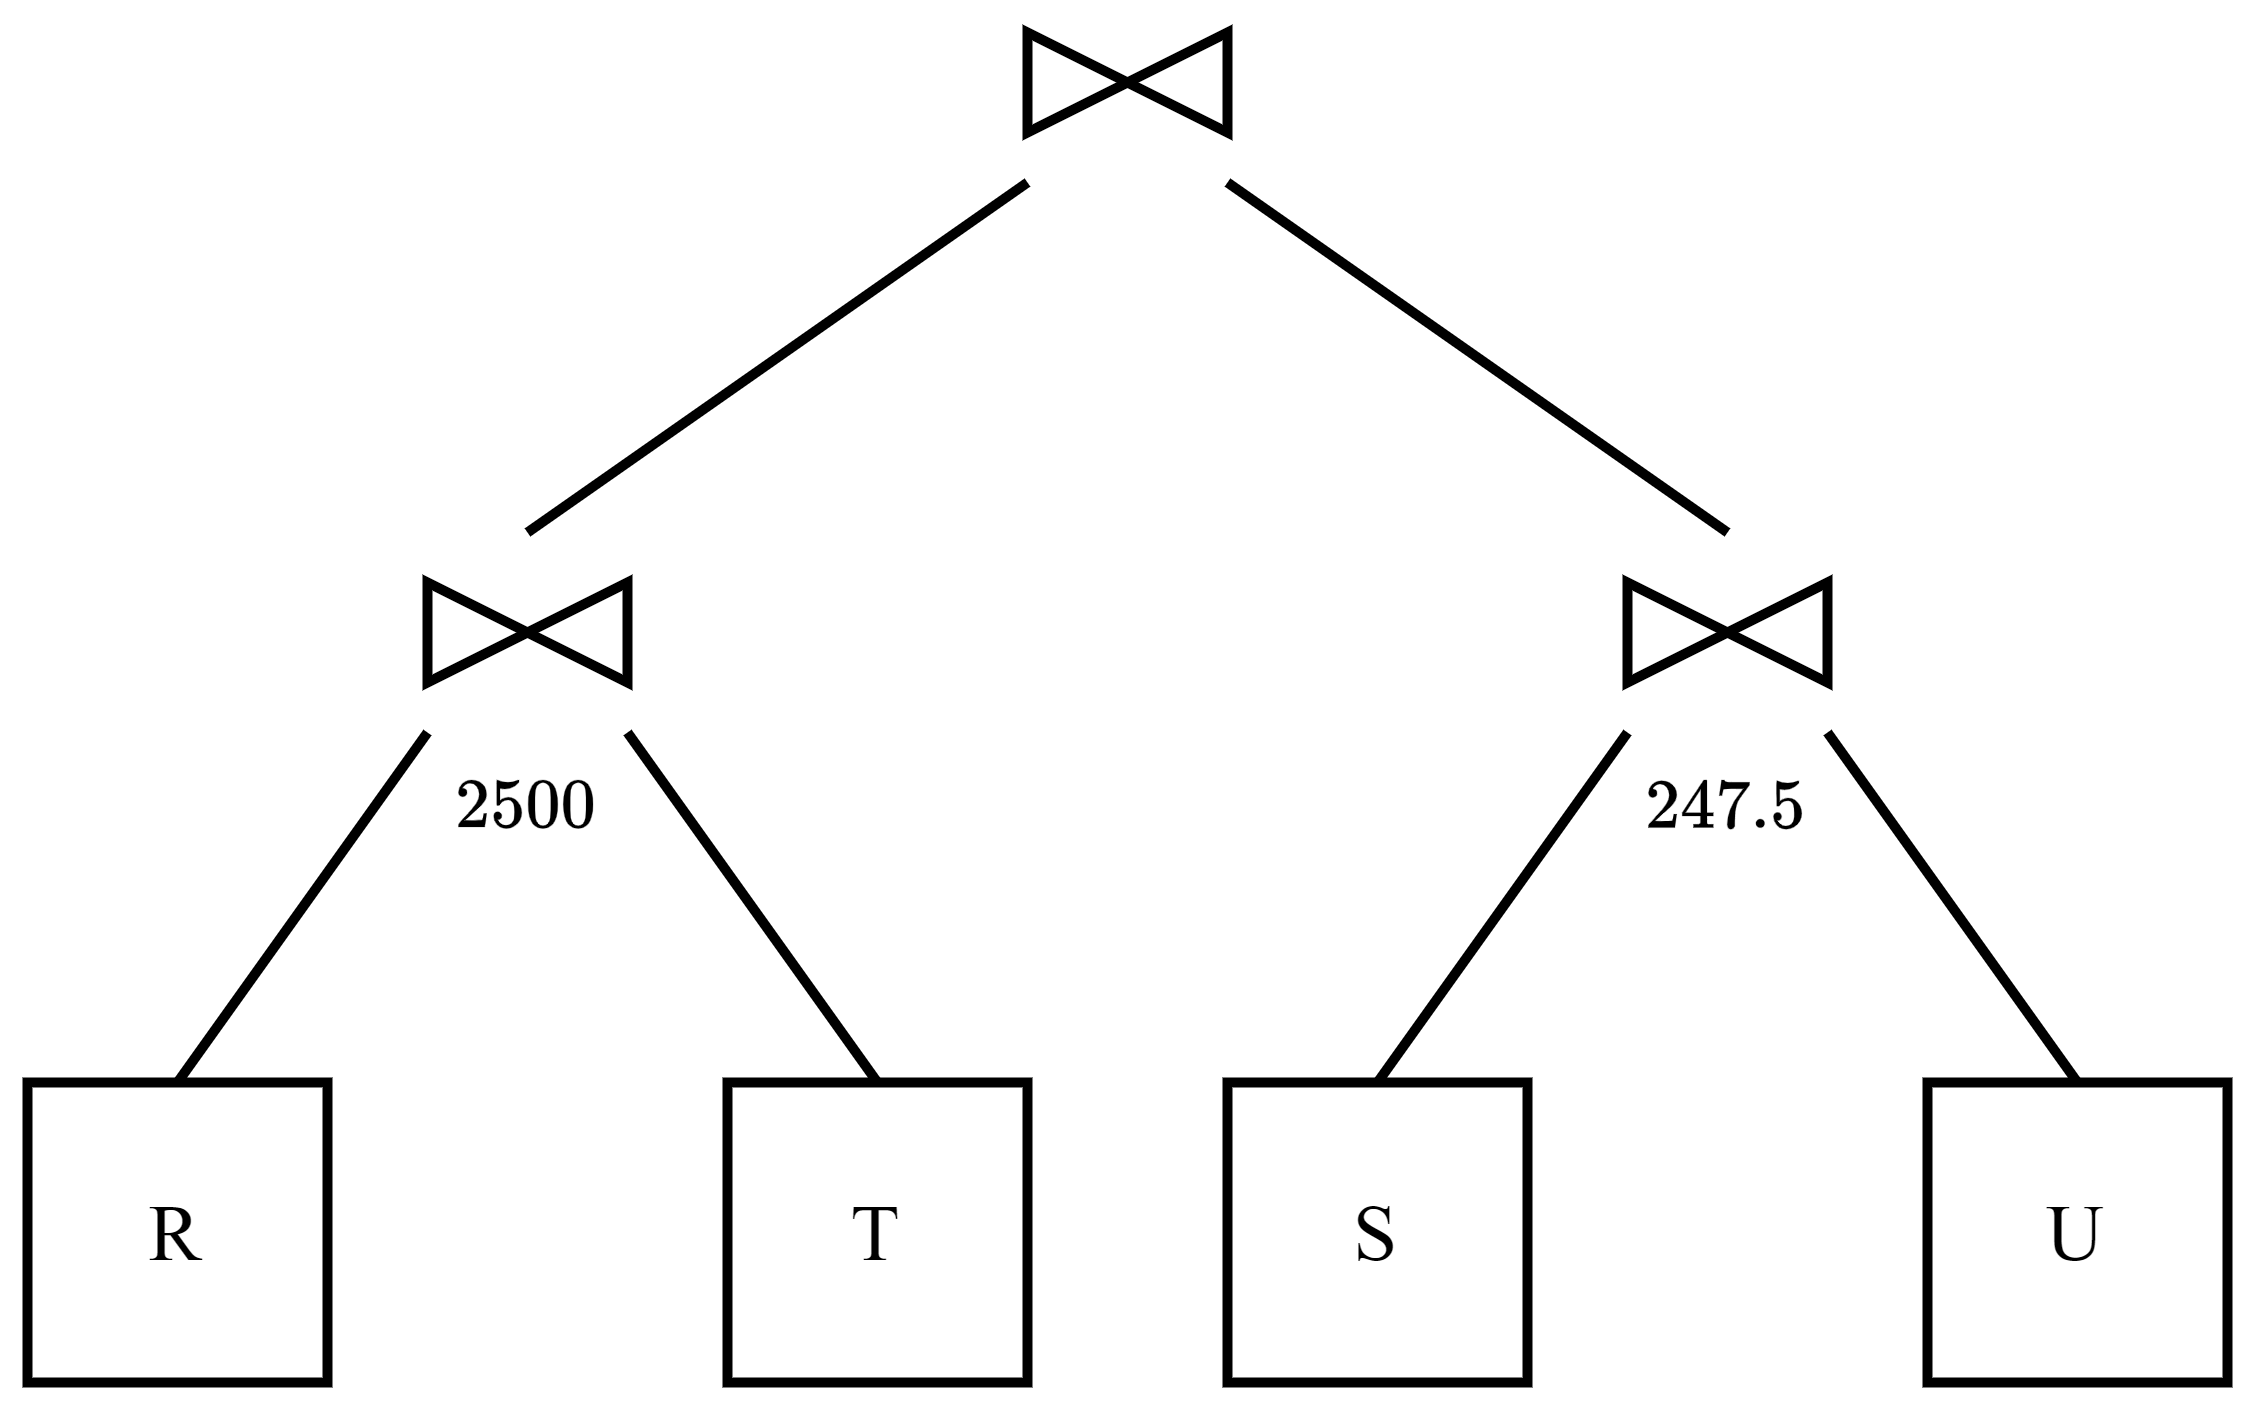
\includegraphics[width=0.5\textwidth]{img/E4-AB2.png}
            \end{figure}

            \newpage
            \item Para $(R \Join U) \Join (S \Join T)$
            \begin{figure}[H]
                \centering
                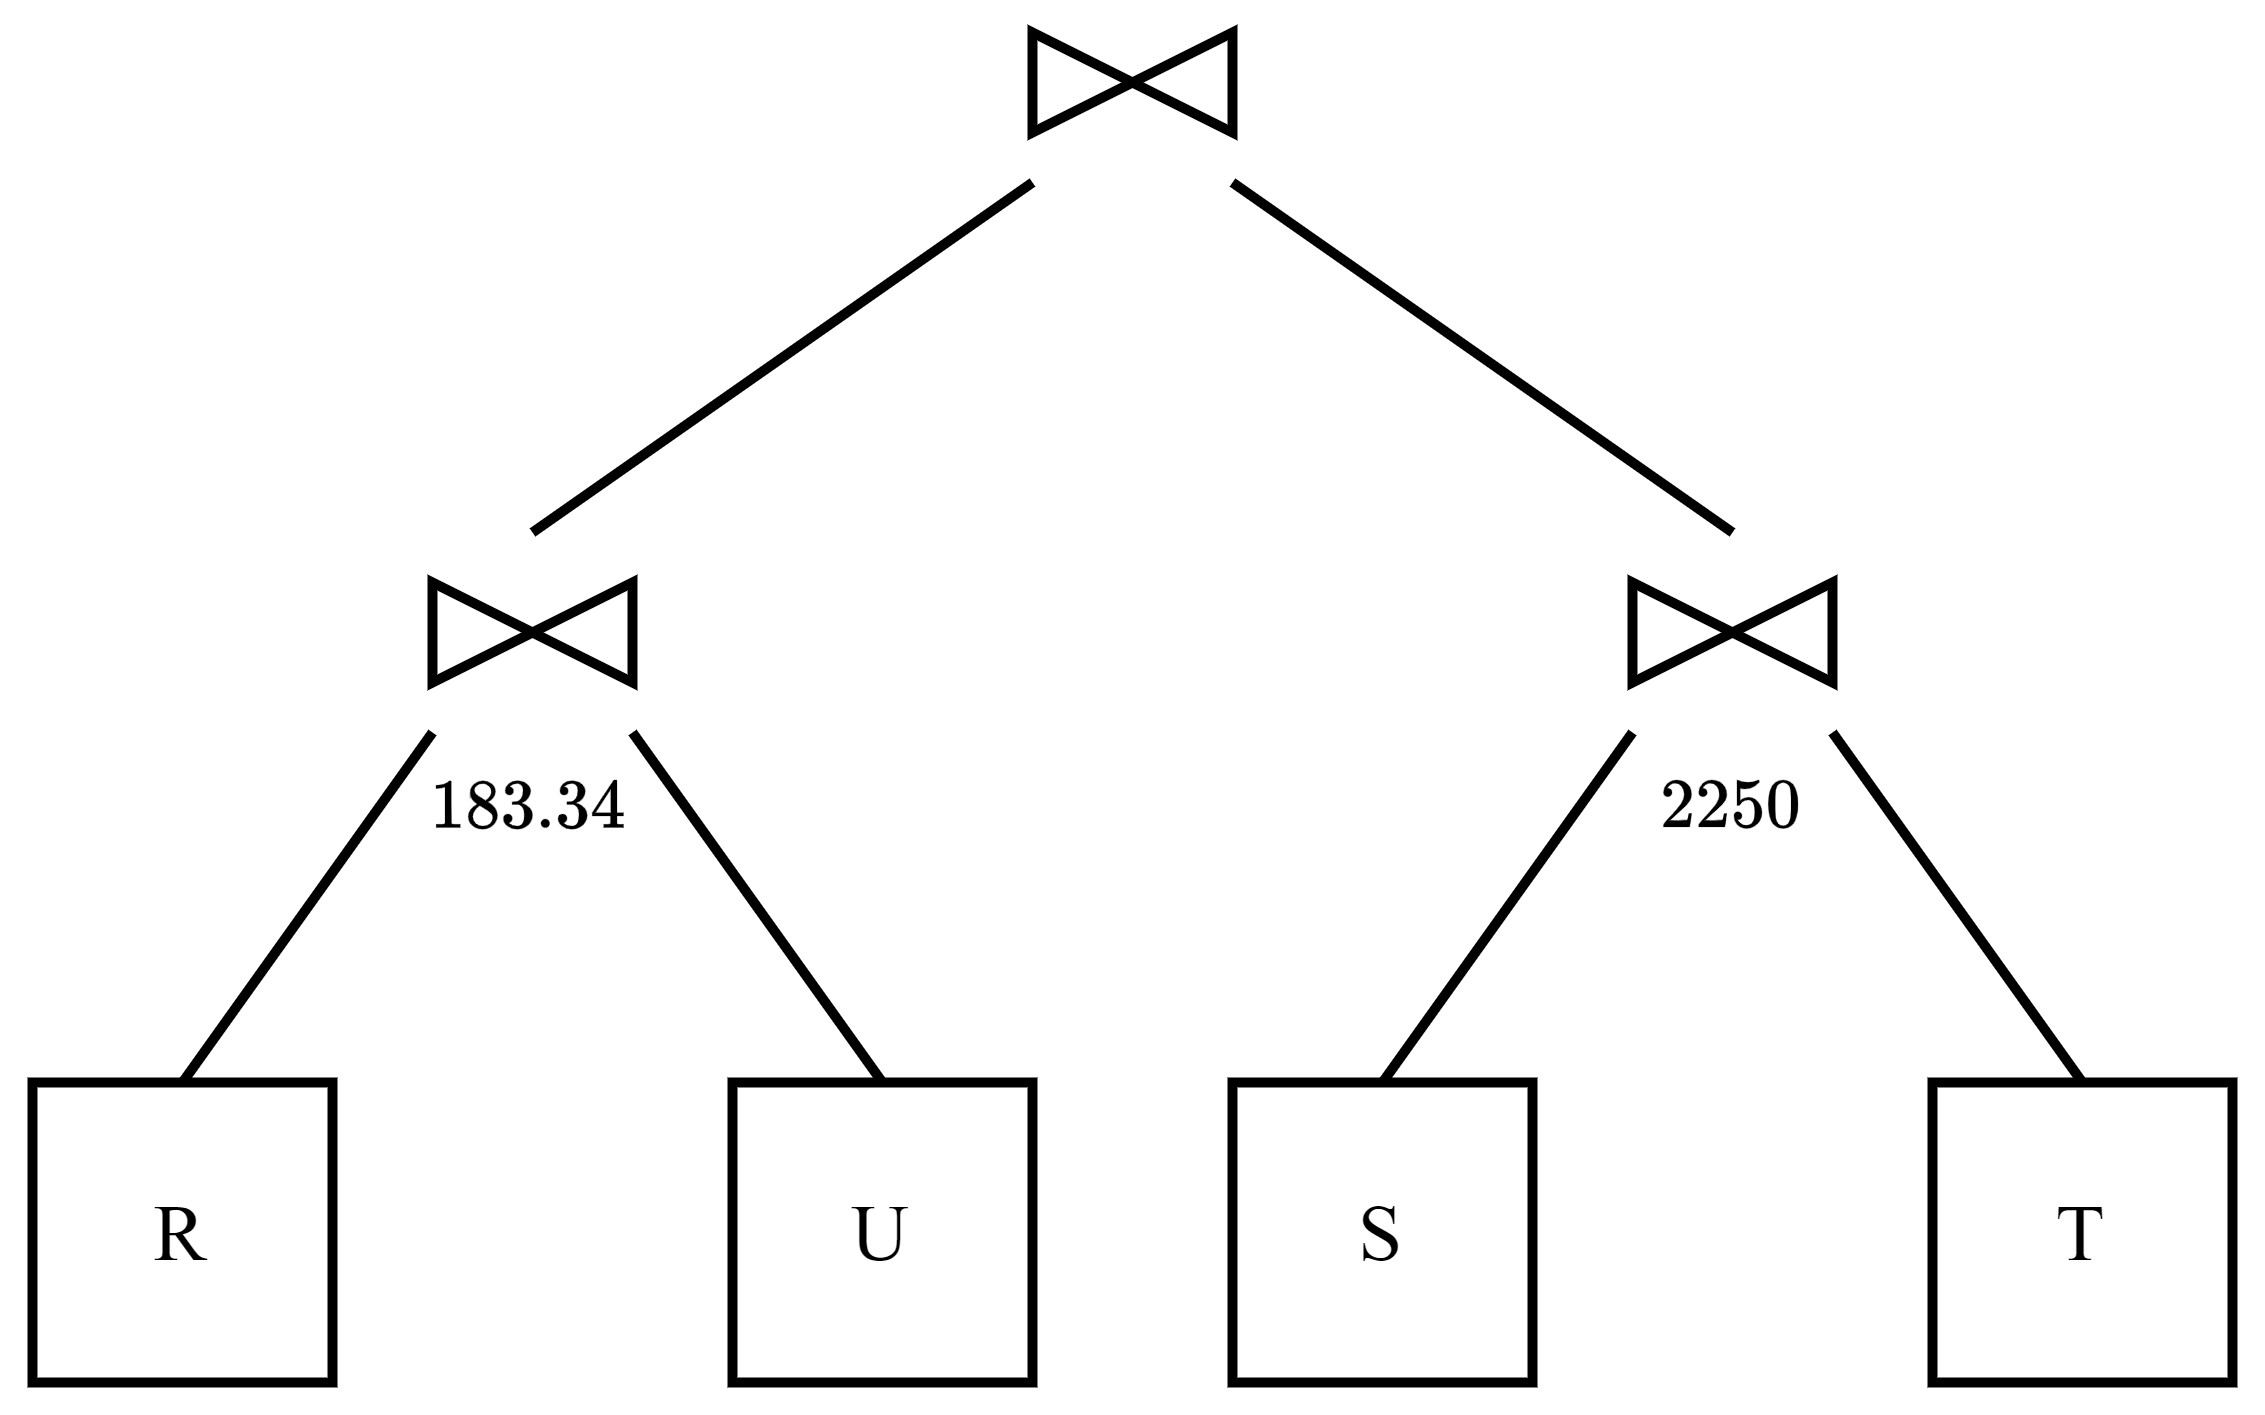
\includegraphics[width=0.5\textwidth]{img/E4-AB3.png}
            \end{figure}
        \end{itemize}
        
        \textbf{Agrupando tenemos que el costo es:}
        \begin{itemize}
            \item $(R \Join S) \Join (T \Join U) = 5.5 + 4.5 = 10$ *
            \item $(R \Join T) \Join (S \Join U) = 2500 + 2475 = 4975$
            \item $(R \Join U) \Join (S \Join T) = 2250 + 183.34 = 2433.34$
        \end{itemize}

        \begin{equation*}
            \therefore \quad \text{El mejor plan es: } (R \Join S) \Join (T \Join U)
        \end{equation*}
    \end{enumerate}

\end{enumerate}
\end{document}